%!TEX root = ../report.tex

\newcommand\scalemath[2]{\scalebox{#1}{\mbox{\ensuremath{\displaystyle #2}}}}


\begin{document}
    \chapter{Evaluation and Experimental Result}
	\label{chap:evaluationandresult}
    The evaluation and experimental result chapter contain the metrics used to evaluate the conducted experiment and the discussion on the research questions. The results of the research question are answered in the subsequent sections, listing the result in a table. Three research questions answered in the section are the results of the state-of-the-art temporal fusion techniques, how the results are compared to each other, and finally, the cross-transfer of the temporal fusion techniques from depth estimation to semantic segmentation. The model is trained and evaluated on three datasets Scannet \cite{79_dai2017scannet}, Virtual Kitti \cite{80_cabon2020vkitti2}, and VIODE \cite{81_minodaRAL2021} datasets. 
    
    \section{Evaluation Metric}
    
    The proposed model needs to be validated to understand the impact of the newly trained model. To validate the model, different evaluation metrics are proposed. The description of the proposed model is listed below.
    
    \subsection{Pixel Accuracy}
    
    Pixel accuracy is commonly defined as the percent of pixels in an image correctly classified into a particular class. Accuracy is defined below
    
    $
    {\bf Accuracy } = \scalemath{2}{\frac{TP+TN}{TP+TN+FP+FN}}
    $
    
    where
     
    $TP$ = True Positive 
    
    $TN$ = True Negative
    
    $FP$ = False Positive
    
    $FN$ = False Negative
    
    
    Per class mean pixel accuracy (mPA)
    
    Per class mean pixel accuracy is the average pixel accuracies of all the classes.
    
    Pixel accuracy (PA) and Mean pixel accuracy (mPA) can also be defined below \cite{84_ulku2022survey}
    
    $
    {\bf PA } = \scalemath{2}{\frac{\sum_{j=1}^{k} n_{jj}}{\sum_{j=1}^{k} t_j} }
    $
    
    $
    {\bf mPA } = \scalemath{2}{\frac{1}{k} \frac{\sum_{j=1}^{k} n_{jj}}{\sum_{j=1}^{k} t_j}}
    $
    
    where $n_{jj}$ is the total number of pixels both classified and labeled as class $j$. 
    
    \subsection{IoU}
    
    Intersection over Union (IoU), also known as the Jaccard index, quantifies the overlapping between the target mask and the predicted output. In other words, the number of standard pixels between the target and prediction masks by the total number of pixels that exist between the masks \cite{83_iou}. A pictorial representation of the same is presented in Fig \ref{fig:IoU}
    
    \begin{figure}[h]
    	\centering
    	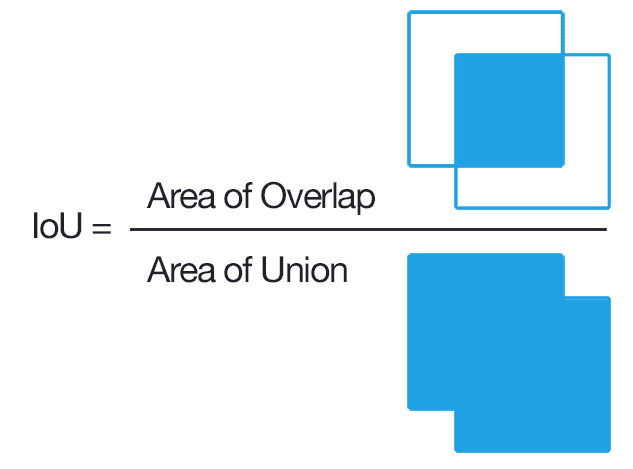
\includegraphics[width=12cm]{images/IoU.png}
    	\caption{IoU. Courtesy of \cite{82_iou}}
    	\label{fig:IoU}
    \end{figure}  
	
	IoU is calculated for each class separately and then averaged over all the classes to provide mean IoU.  
	
	$
	{\bf IoU} = \scalemath{2}{\frac{\sum_{j=1}^{k} n_{jj}}{\sum_{j=1}^{k} (n_{ij}+n_{ji}+n_{jj})}, i \neq j }
	$

	where $ n_{ij}$ is the pixels which are labeled as class i but classified as class j and $n_{ji}$ is the total number of pixels labeled as class j, but classified as class i. \cite{84_ulku2022survey}
	
	$
	{\bf mIoU} = \scalemath{2}{\frac{1}{k} \sum_{j=1}^k \frac{n_{ij}}{n_{ij}+n_{ji}+n_{jj}},  i \neq j }
	$
	
	Frequency-weighted IoU (FwIoU). It is a metric derived from the mIoU, which weighs each class's importance depending on appearance frequency using $t_j$ \cite{84_ulku2022survey}
	
	$
	{\bf FwIoU} = \scalemath{2} {\frac{1}{\sum_{j=1}^k t_j} \sum_{j=1}^{k} t_j \frac{n_{jj}}{n_{ij}+n_{ji}+n_{jj}}, i \neq j }
	$
    
    \section{Hypothesis}
    
    Semantic segmentation is a vital task in the computer vision domain that assigns labels to every pixel in an image. Semantic segmentation is applied in 2D images, Video data, and 3D or Volumetric data. The video sequence data contains multiple image frames stacked together. Given the high frame rate of the video, the consecutive frames are related to each other due to the overlapping regions in the successive frames. In most semantic segmentation tasks, the segmentation is performed on each frame or the keyframes. Past information can be fused into current step computation by taking the learned features from previous frames \cite{78_hu2020temporally}.
    
    The work hypothesizes that the performance improves by fusing the past information onto the current frame segmentation computation by the following approaches.
    
    (i) Subjecting the latent space encoding of the Unet model to the Gaussian process by taking the pose of the current frame and the previous frame, the performance improves in comparison to segmentation without temporal fusion since the overlapping information present in the past is used for computation of the current frame segmentation.
    
    (ii) Placing the ConvLSTM cell at the latent space encoding of the Unet model to transfer the geometry information from the past to the current step helps improve semantic segmentation performance. 
    
    The approach is cross-transferred from the depth estimation task \cite{52_hou2019multi} \cite{03_duzceker2021deepvideomvs}. 
    
    \section{RQ1: What are the works on state-of-the-art temporal fusion in semantic segmentation?}
	
	Segmentation is the process of assigning pixel labels for a given image. Segmentation can be observed in different contexts, such as Video instance segmentation (VIS), Semantic segmentation of the key frames of a video sequence, Video panoptic segmentation, MRI image segmentation, and autonomous driving scene understanding. Youtube - Video Instance Segmentation (VOS) and Scannet are the standard datasets in the semantic segmentation domain. 

	{ \bf Youtube VIS data}
	Youtube - Video Instance Segmentation (VIS) is a dataset that extends the image instance segmentation from the image to the video domain. The dataset aims to solve the problem of simultaneous detection, segmentation, and tracking problem. Scannet is an RGB-D video dataset containing 2.5 million views with more than 1500 scans. 
	%	\ref{59_starck2005image}
	A paper by Xiang Li et al. [87] explains the temporal fusion for online video instance segmentation. The author introduced the concept of an online video framework with a novel, aware temporal fusion method. A cropping-free temporal fusion approach to model the temporal consistency between video frames. A bottom-up online transformer-based network is used to solve the VIS problem. A transformer layer is introduced in the convolutional neural network (CNN) to include the instance information. An attention layer between the frames is used to extract the instance code for the current frame. A skip connection uses low-level contextual information and dynamic convolution to generate the segmentation map—the CNN feature map and the latent code help to represent instance-aware features jointly. An instance code is an LxD vector to the VIS task, where L is the maximum detected instances number in a frame D is the feature instance for each instance. Inter and Intra frame attention module for fusing the temporal information. The network architecture is presented in Fig \ref{fig:vis}. Three types of attention are code-to-code(c2c), code-to-pixel(c2p), and pixel-to-code(p2c), used to construct the	relationship between the instance code and feature map. Interframes are used to build the temporal correlation and combine contextual features across frames. Interframe c2c, c2p, and p2c are used to construct the temporal information.	

    \begin{figure}
		\centering
		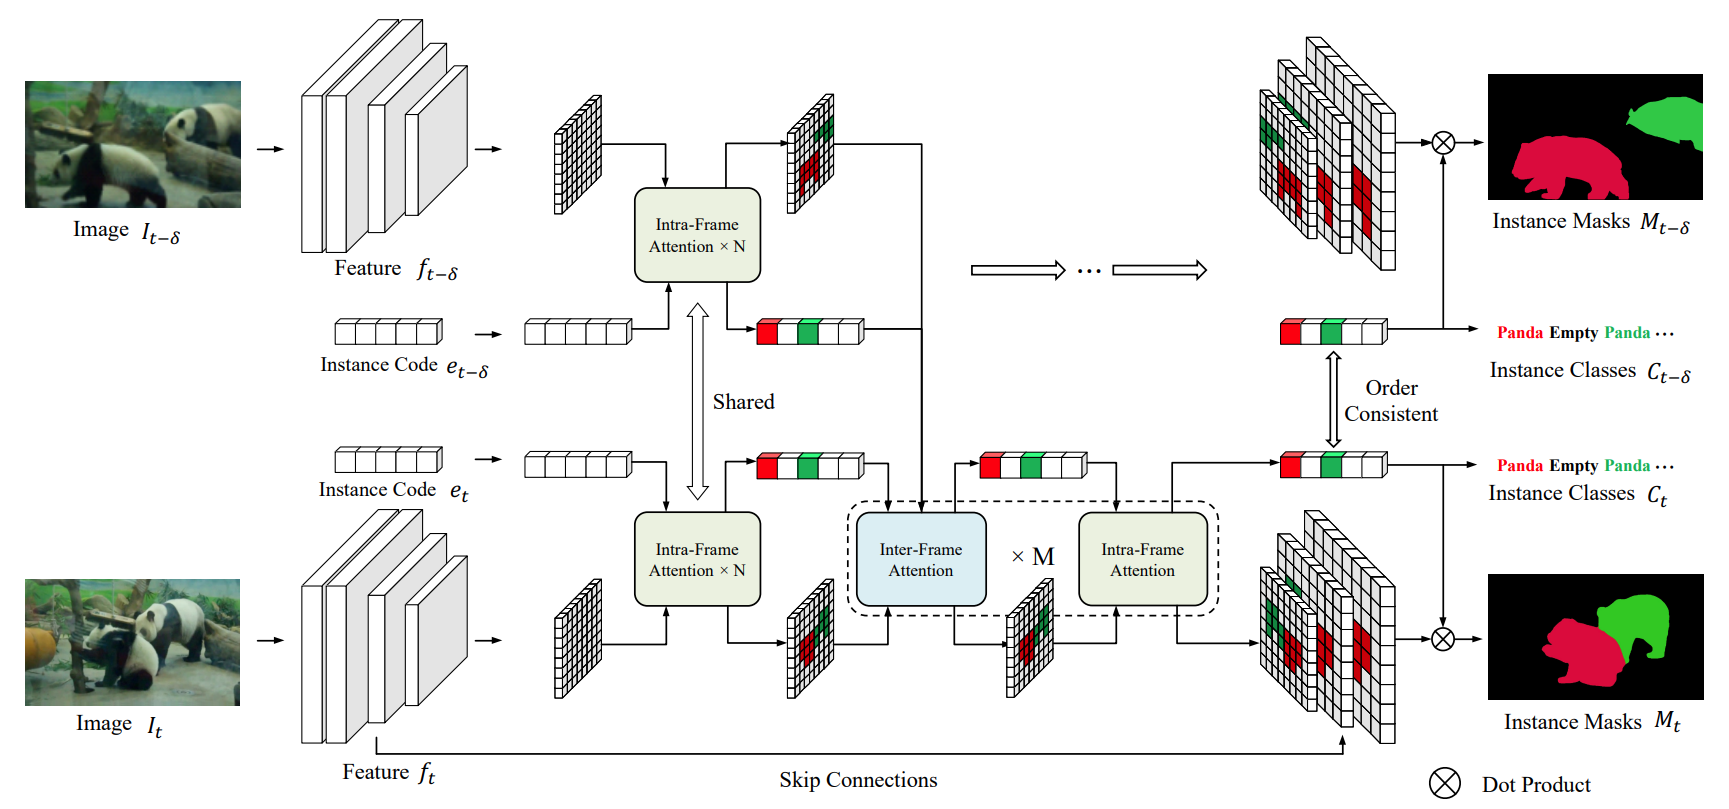
\includegraphics[width=13cm]{images/VIS.png}
		\caption{VIS proposed framework. Courtesy of [87]}
		\label{fig:vis}
	\end{figure}
%	\ref{87_heo2022vita}
	Miran Heo et al. [88] worked on video instance segmentation via Object Token Association (VITA). The work effectively understands the video through the object-centric tokens. The VITA model requires a frame-level detector. The frame-level detector localizes instances using masks without bounding boxes. Two features are generated for the frame-level predictions: a) dynamic 1x1 convolution weight from the frame queries f b) per-pixel embeddings from the pixel decoder. The dot product between the two embeddings is taken in the frame-level predictions. The end-to-end video instance segmentation method VITA is divided into three stages. Firstly, VITA works with the frame-level detector in a frame-independent manner. No computation between the frames is involved. The frame queries that hold the object-centric information are collected throughout the video sequence, and an object encoder is used to build the video-level information between the frames. Moreover, thirdly the decoder combines the information from the frame and video queries which is finally used to find the object mask in the video frames. 
	
	\begin{figure}
		\centering
		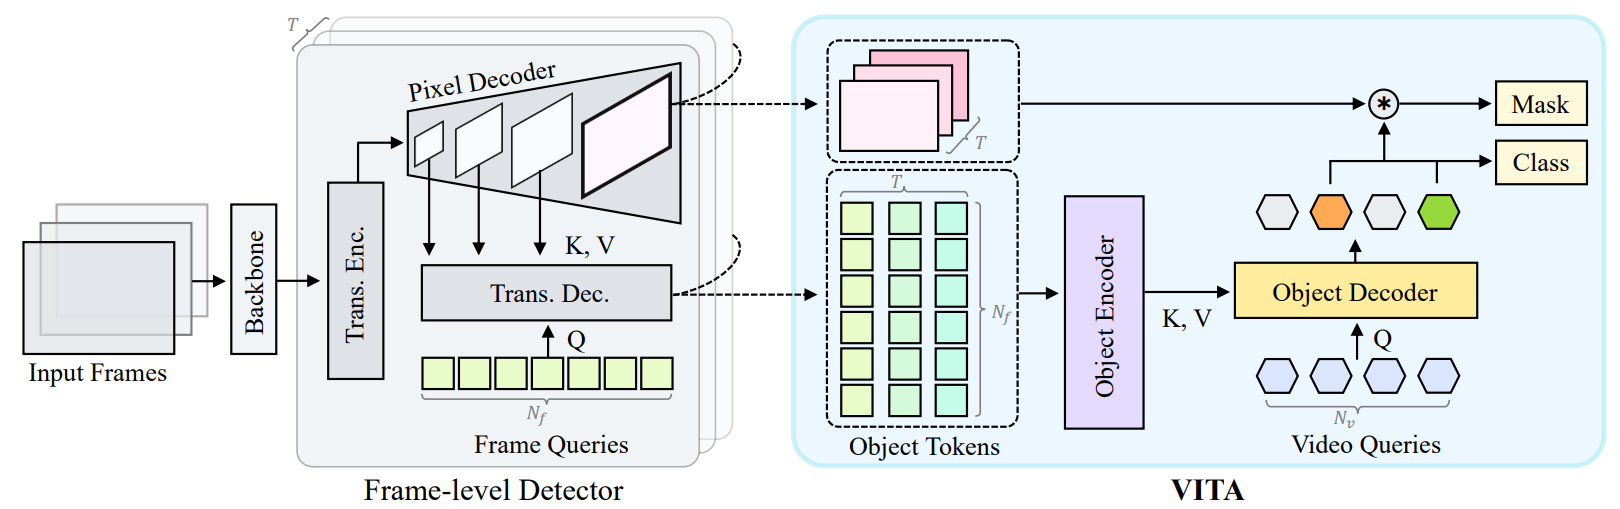
\includegraphics[width=13cm]{images/VITA.png}
		\caption{The frame level detector takes frame queries and mask features, generates the embeddings, and pass onto the VITA model for mask prediction. Constructing the temporal interactions between the frame queries captures the object-aware knowledge in the spatial scenes. Finally, mask trajectories are obtained from the VITA model. Courtesy of [88]}
		\label{fig:vita}
	\end{figure}
%	\ref{88_huang2022minvis}
	A minimal video instance segmentation (MinVIS) by De-An Huang et al. [89] does not require video-based training and can be applied directly to images containing sparse image instance segmentations annotations. MinVIS is a two-stage approach: 1) Independent image instance segmentation on each frame and 2) Instance association between the frames. Image Instance Segmentation has three unique main components a)Encoder to extract features from the image b) Transformer decoder, used to process the output of the image encoder to update the query embeddings c) Prediction head takes the query embeddings to predict the output. Association between the instance segmented frames is calculated by bipartite matching of the respective query embeddings.   
	
	\begin{figure}
		\centering
		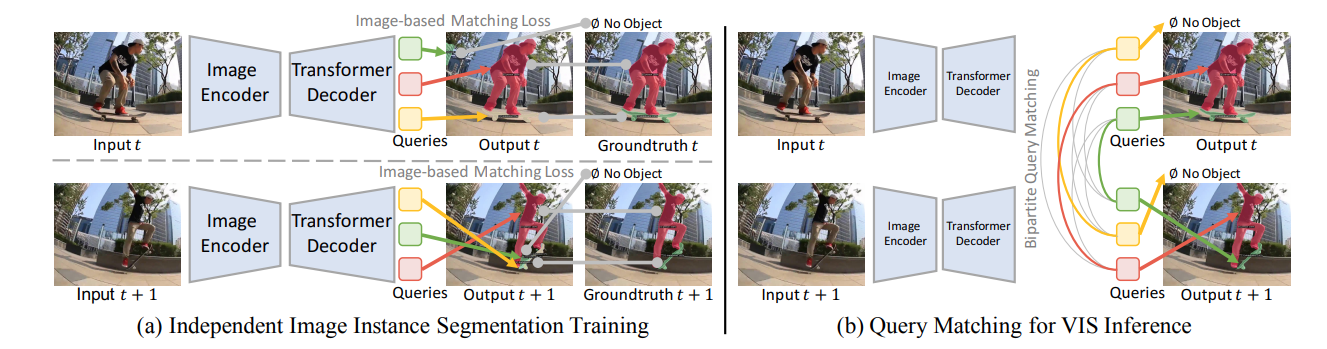
\includegraphics[width=13cm]{images/minVIS.png}
		\caption{(a) MinVIS trained on query-based segmentation individually for every frame. (b) Inference of the video instance segmentation from the segmented image using bipartite matching of the query embeddings. Courtesy of [89] }
		\label{fig:minVIS}
	\end{figure}
%	\ref{89_cheng2021mask2former}
	The state-of-the-art segmentation models solve mask classification in image segmentation problems. B. Cheng et al. [90] proposed a method to process the video directly rather than the image. This is achieved by feeding the Mask2Former with 3D spatiotemporal features and predicting the 3D volume to track each object instance across time. The Mask2Former works as a general image segmentation model for data with single frames and for data with more than one frame the model segments and tracks instances across frames. 

	\begin{figure}
		\centering
		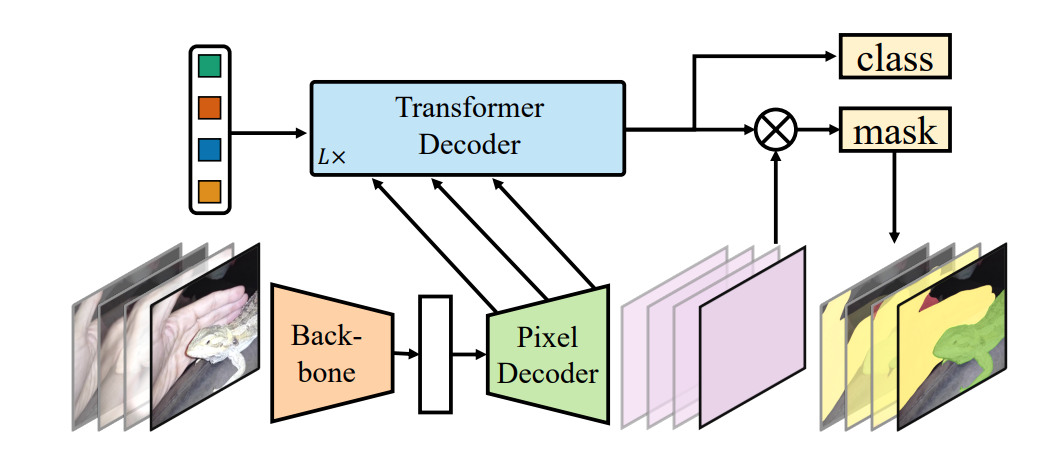
\includegraphics[width=13cm]{images/mask2former.png}
		\caption{ A mask2former with video instance segmentation. Courtesy of  [90]}
		\label{fig:mask2former}
	\end{figure}	
	
    \section{RQ2: How are the results from RQ1 compared with each other to perform temporal fusion?}
    
   	All of the above mentioned approaches are trained and tested on the Youtube VIS datasets. The performance of the models are tabulated in table \ref{tab:sota_ytube_vis}.
   
	\begin{table}[h]
   		\begin{center}
   			\begin{tabular}{ | l | l| l| l| l| p{2cm} |}
   				\hline
   				
   				\cellcolor{purple!30}Method & \cellcolor{purple!30}AP & \cellcolor{purple!30}AP50 & \cellcolor{purple!30}AP75 & \cellcolor{purple!30}AR1 & \cellcolor{purple!30}AR10 \\ \hline
%   				\ref{86_li2022hybrid}
   				HIATF for VIS 2019 [87] & 41.3 & 61.5 & 43.5 & 42.7 & 47.8 \\ \hline
%   				\ref{87_heo2022vita}
   				VITA ResNet-50 2019 [88]  & 49.8 & 72.6 & 54.5 & 49.4 & 61.0  \\ \hline
%   				\ref{87_heo2022vita}
   				VITA ResNet-101 2019 [88]  & 51.9 & 75.4 & 57.0 & 49.6 & 59.1 \\ \hline
%   				\ref{87_heo2022vita}
   				VITA Swin-L 2019 [88]  & 63.0 & 86.9 & 67.9 & 56.3 & 68.1 \\ \hline
%   				\ref{87_heo2022vita}
   				VITA 2021 [88]  & 45.7 & 67.4 & 49.5 & 40.9 & 53.6 \\ \hline
%   				\ref{88_huang2022minvis}
   				Min VIS 2019 [89] & 61.6 & 83.3 & 68.6 & 54.8 & 66.6 \\ \hline
%   				\ref{88_huang2022minvis}
   				Min VIS 2021 [89] & 55.3 & 76.6 & 62.0 & 45.9 & 60.8 \\ \hline
%   				\ref{89_cheng2021mask2former}
   				Mask2former 2019 [90]  & 60.4 & 84.4 & 67.0 & - & - \\ \hline
%   				\ref{89_cheng2021mask2former}   
   				Mask2former 2021 [90]  & 52.6 & 76.4 & 57.2 & - & - \\ \hline
   				\hline
   			\end{tabular}
   			\caption{Comparison of temporal fusion model performance with respect to Youtube VIS dataset}
   			\label{tab:sota_ytube_vis}
   		\end{center}
   	\end{table}
    
    \section{RQ3: How to cross-transfer the temporal fusion technique to semantic segmentation?}
    
    The U-net model was developed to categorize biomedical images. Currently, the model is used in other application areas as well. The original network is mainly based on the data augmentation strategy. The network consists of an encoder and decoder along with the interconnection between different layers of encoder and decoder. The expanding path of the U-net model helps capture the objects' location in the image. The vanilla U-net model code is referenced from the Kaggle competition \cite{85_kag_challenge}. The result presented below is for the vanilla U-net model trained on the scannet dataset \cite{79_dai2017scannet}. The model is trained for 300 epochs. The plain vanilla model is trained with a neural network-based unet model. The experiment is conducted in three ways
    \begin{itemize}
    	\item Considering all the classes
    	\item Containing only two classes by combining the low pixel distribution classes together (Wall and Other)
    	\item Containing three classes by combining classes with low pixel distribution (Wall, Furniture, and Other)
    \end{itemize}
    
    
    The parameter used to train a plain unet model is tabulated in \ref{label}.
    
    \subsection{Combining scannet dataset classes for experiment}
    
	There are 41 classes [ \ref{table:Classes in scannet_1} , \ref{table:Classes in scannet_2} , \ref{table:Classes in scannet_3}] present in the entire Scannet dataset. 

	To experiment, 185 indoor video sequence data are considered. The distribution of the entire scannet data classes is presented in Fig \ref{fig:scannet_class}. Of 185 sequences, 149 sequences are taken for training and the remaining 36 for testing. The distribution of pixels in the training data and testing data represented in Fig \ref{fig:scannet_all_classes}.
	
	The pixel distribution of the scannet dataset classes is not uniform. Experiments were conducted in three ways; in the first approach, all the classes were considered for experimenting, and no combining of the classes. In the second approach, all the classes other than the wall class are combined to assign a class label of "zero," and the "Wall" class is chosen as the second class. The distribution of the pixels is depicted in Fig \ref{fig:scannet_two_classes}.
	The Wall, Furniture, and Other classes combined have a high pixel distribution; hence all the furniture classes are combined as class 2nd, Wall as the first class, and the remaining classes are combined into 0th class as Other classes, resulting in three unique classes. The distribution of the three classes is presented in Fig \ref{fig:scannet_three_classes}.
    
    %------------------------------------------------------------------------------------------------------
    \begin{figure}
    	\centering
    	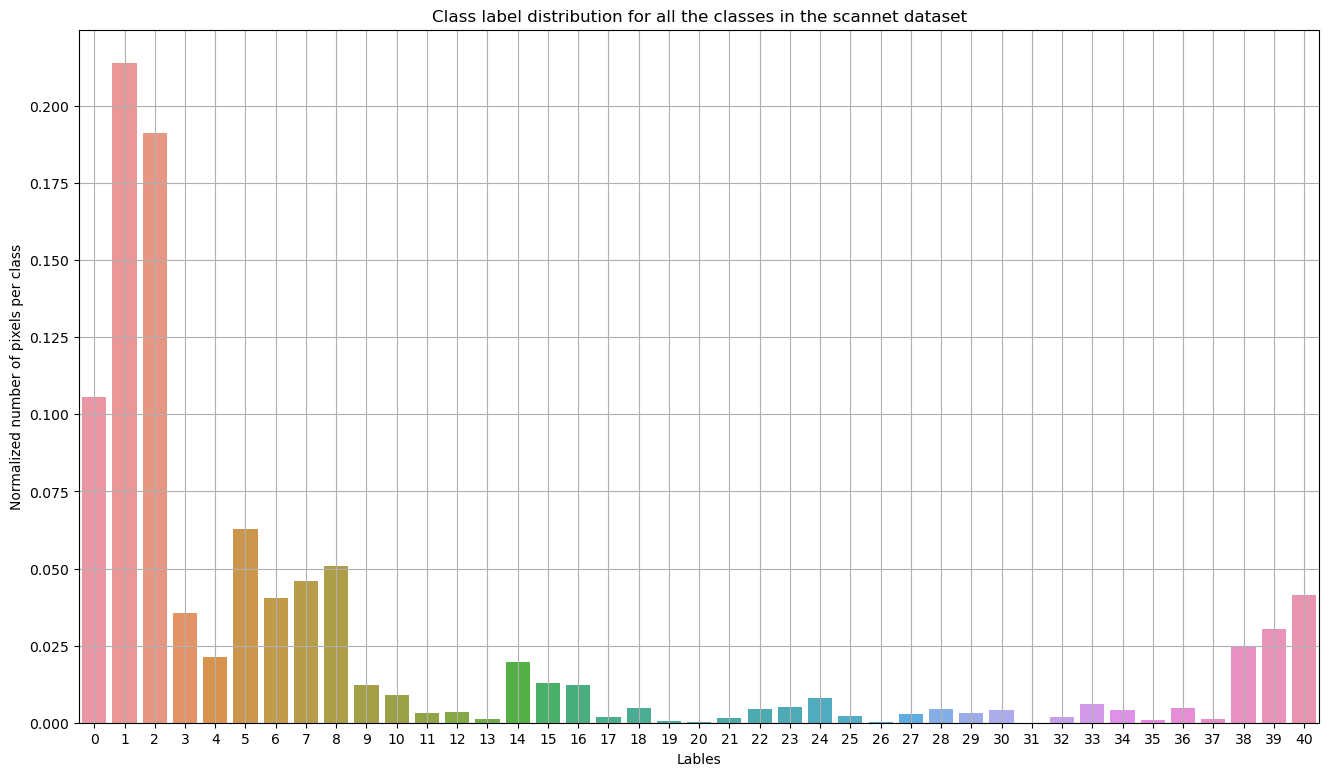
\includegraphics[width=13cm]{images/scannet_data_class_distribution.png}
    	\caption{Per class pixel distribution of the entire scannet dataset}
    	\label{fig:scannet_class}
    \end{figure} 
    
    \begin{figure}%
    	\centering
    	\subfloat[\centering Per class pixel distribution of the training dataset pixel class label ]{{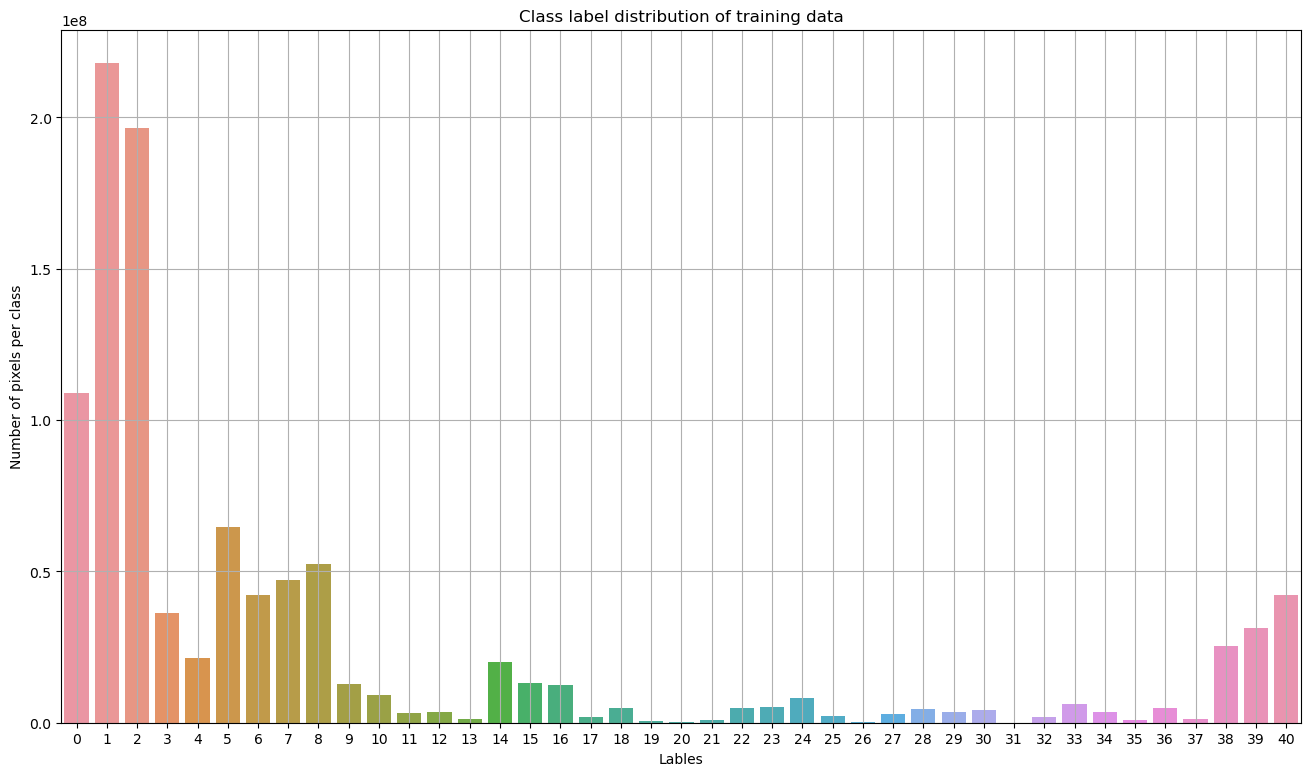
\includegraphics[width=7cm]{images/scannet_training_data_class_distribution.png} }}%
    	\qquad
    	\subfloat[\centering Per class pixel distribution of the testing dataset pixel class label]{{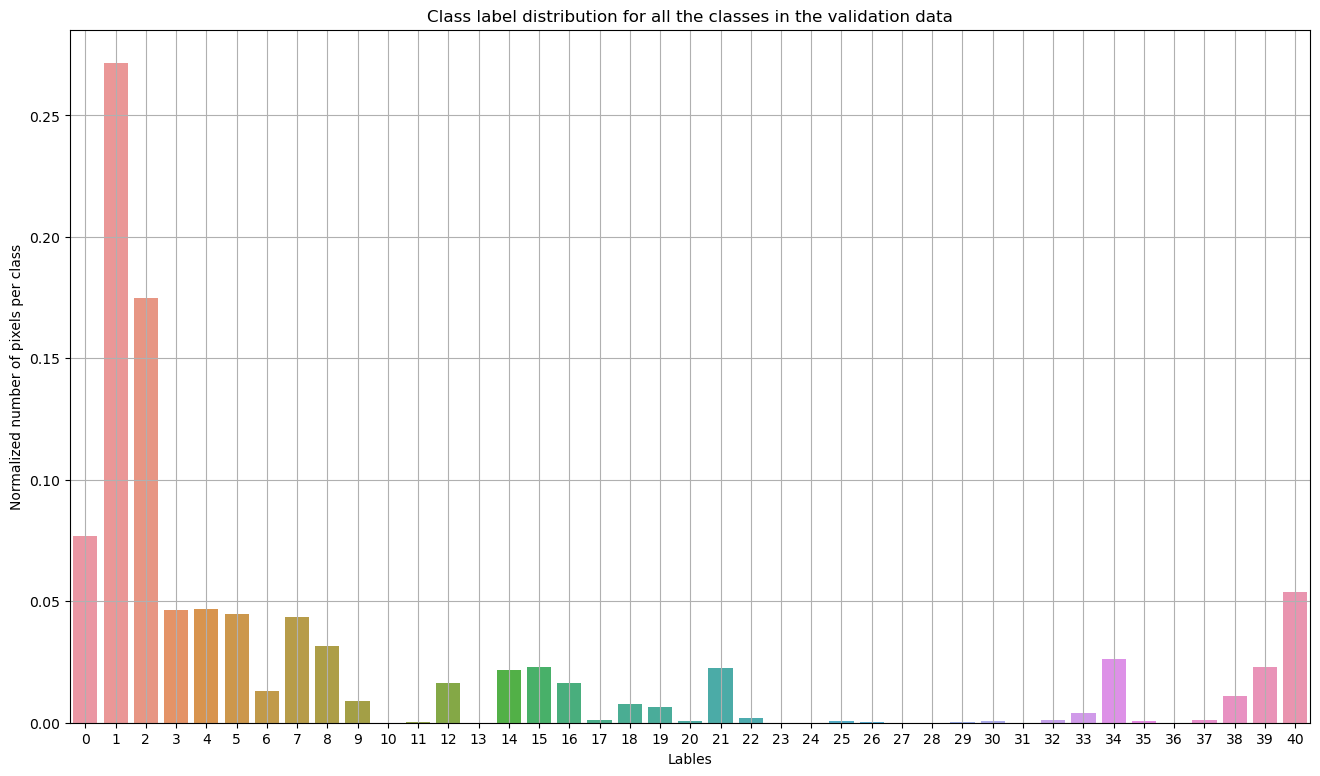
\includegraphics[width=7cm]{images/scannet_testing_data_class_distribution.png} }}%
    	\caption{Pixel distribution for the scannet data containing all the classes}%
    	\label{fig:scannet_all_classes}%
    \end{figure}
    
    \begin{figure}%
    	\centering
    	\subfloat[\centering Per class pixel distribution of the training dataset pixel class label ]{{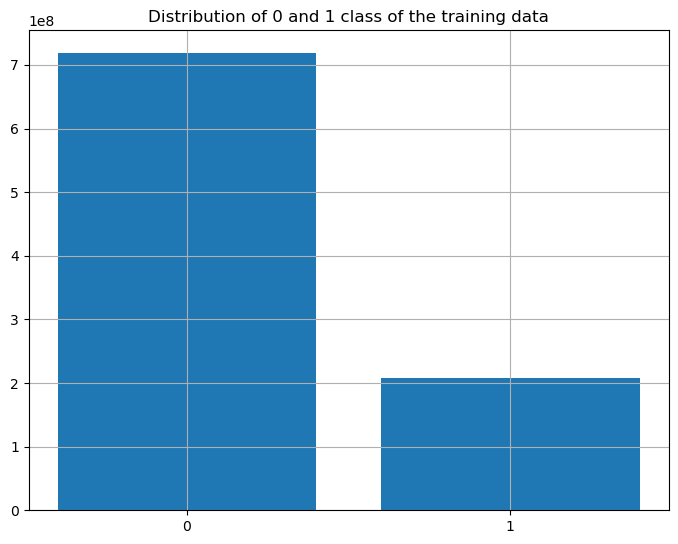
\includegraphics[width=7cm]{images/scannet_training_data_class_distribution_two_classes.png} }}%
    	\qquad
    	\subfloat[\centering Per class pixel distribution of the testing dataset pixel class 	label]{{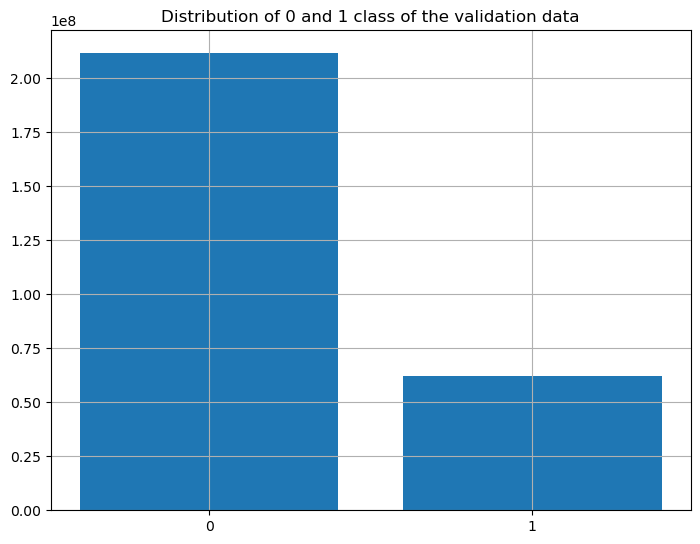
\includegraphics[width=7cm]{images/scannet_testing_data_class_distribution_two_classes.png} }}%
    	\caption{Pixel distribution for the scannet data for two classes}%
    	\label{fig:scannet_two_classes}%
    \end{figure}

   	\begin{figure}%
    	\centering
    	\subfloat[\centering Per class pixel distribution of the training dataset pixel class label ]{{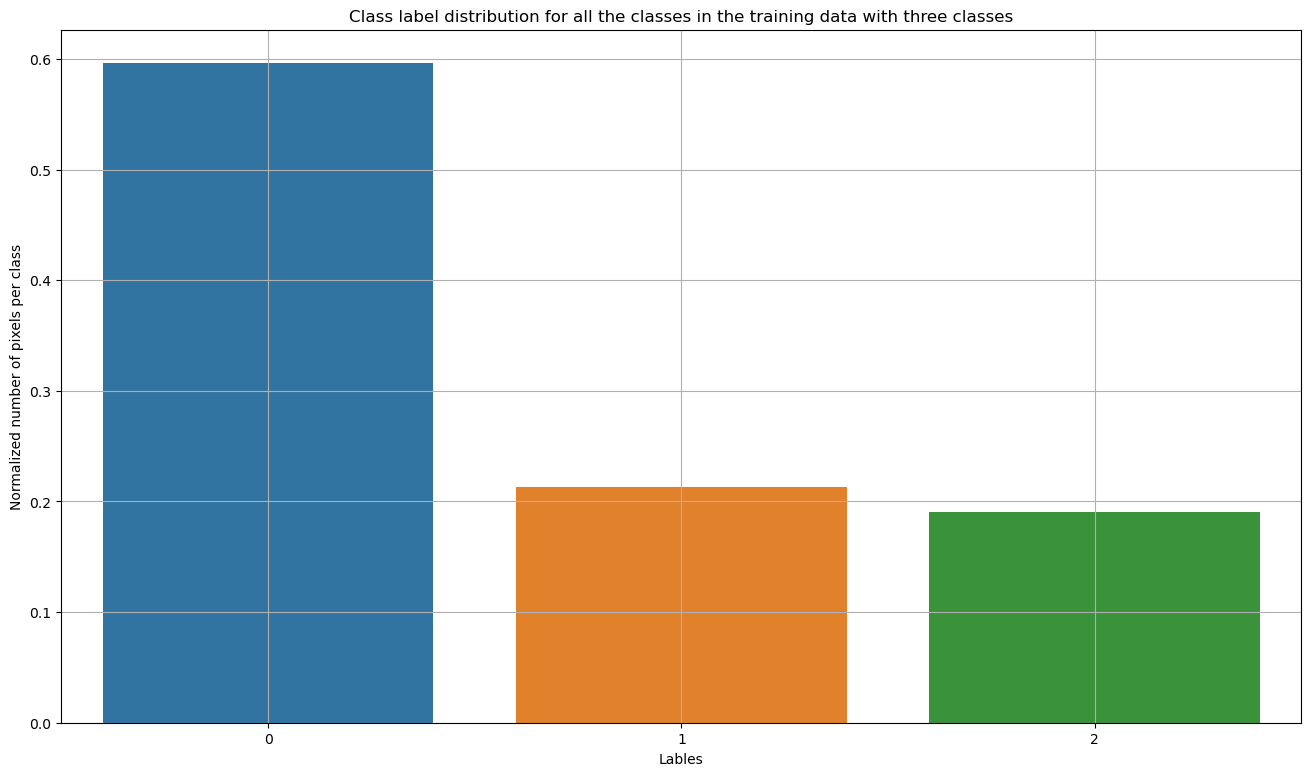
\includegraphics[width=7cm]{images/scannet_training_data_class_distribution_three_classes.png} }}%
    	\qquad
    	\subfloat[\centering Per class pixel distribution of the testing dataset pixel class 	label]{{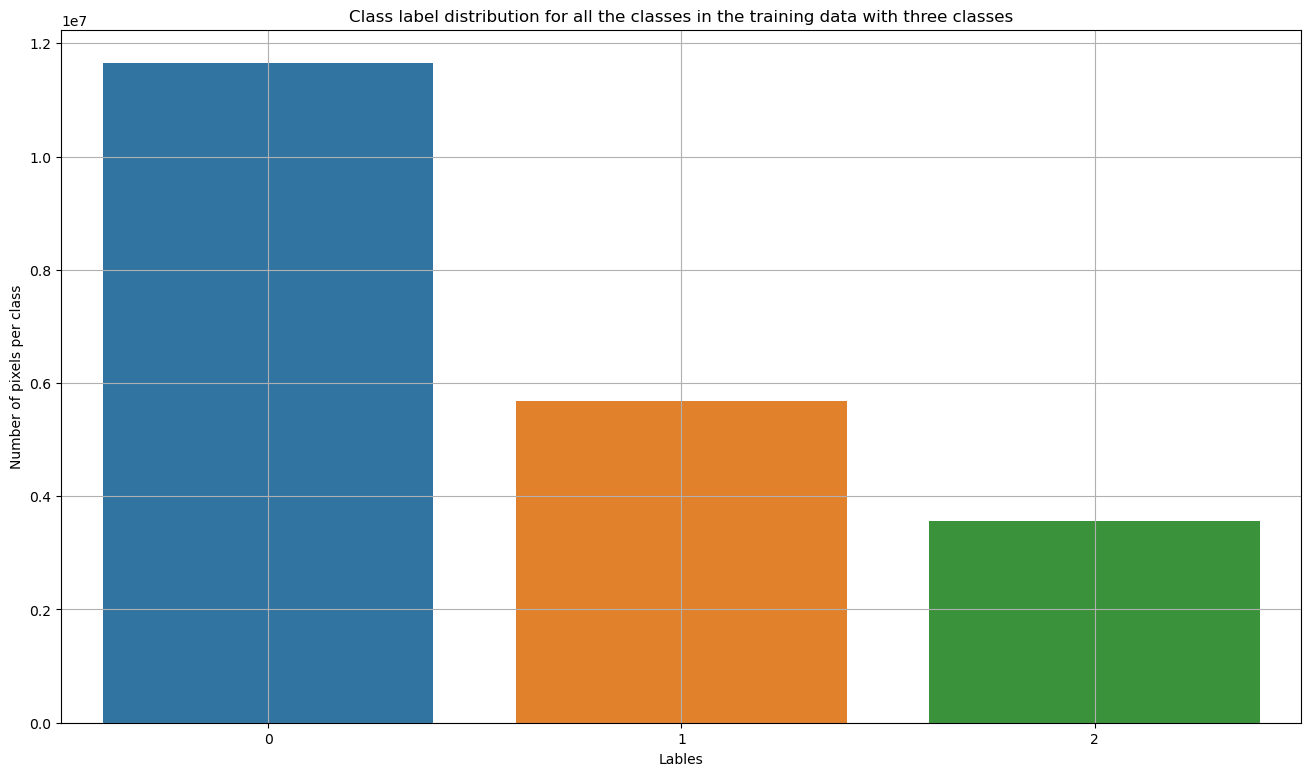
\includegraphics[width=7cm]{images/scannet_testing_data_class_distribution_three_classes.png} }}%
    	\caption{Pixel distribution for the scannet data for three classes}%
    	\label{fig:scannet_three_classes}%
    \end{figure}
    %---------------------------------------------------------------------------------------------------------
    \subsection{Distance and Kernel matrix}
	
	A distance matrix is a square matrix that represents the distance between a pair of objects. Distance matrix can be constructed from the pose information of the captured video sequence. The closer the two frames are in a sequence, the distance between them is; the smaller same can be represented with the matrix plot. Two types of the distance matrix are plotted in Fig \ref{fig:ordered_D_and_K} and \ref{fig:unordered_D_and_K}. In the first type of plot, an ordered frames pose is represented in the x and y-axis. The distance of the pose with respect to itself is zero, and as the frame number increases, the distance keeps increasing. In the second type of unordered pose plot, the frame's pose is shuffled and presented as the matrix plot. These pictures represent the distance of one frame to the other. 
	
	\begin{figure}[h]
		\centering
		\subfloat[\centering Ordered set of images]{{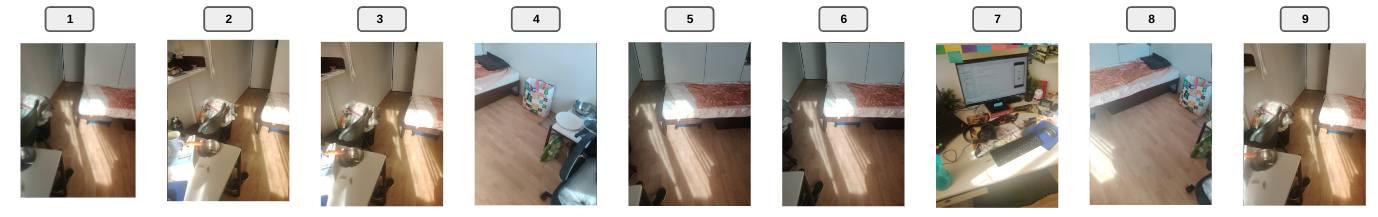
\includegraphics[width=14cm]{images/ordered_images.jpg} }}%
		\qquad
		\subfloat[\centering Unordered set of images label]{{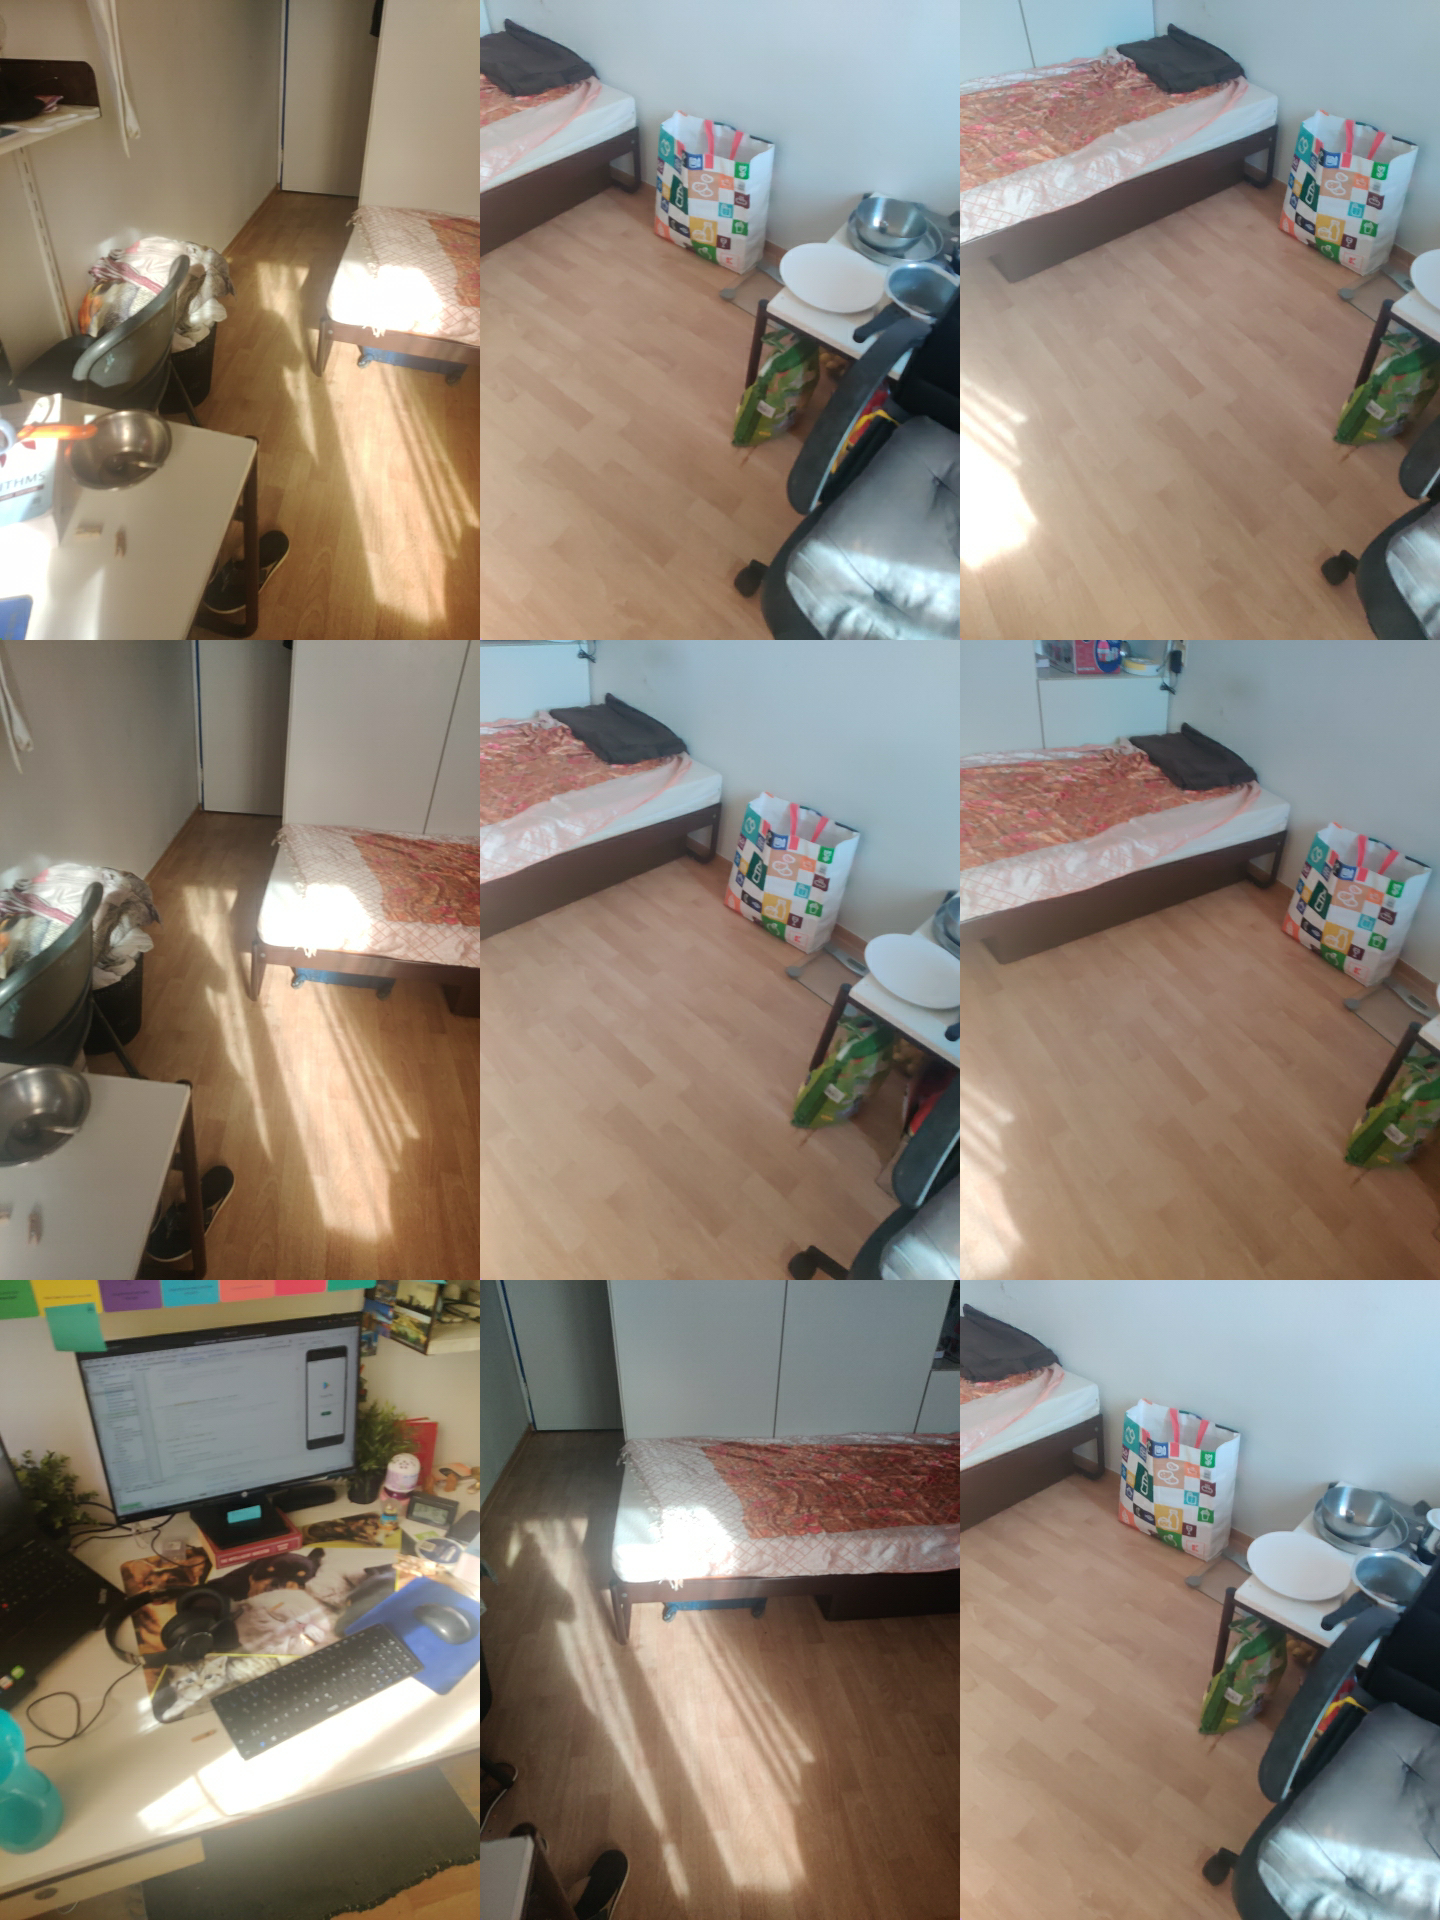
\includegraphics[width=14cm]{images/unordered_images.jpg} }}%
		\caption{Ordered and Unordered set of images}%
		\label{fig:ordered_and_unordered_images}%
	\end{figure}
	
	The distance matrix is used to construct the kernel of the Gaussian process. The kernel represents the similarity or correlation between the two data points. Closer data points in the distance space have a high correlation, and further away data points have a low correlation, and the same can be observed in the plotting of the kernel matrix as a heatmap in Fig \ref{fig:ordered_D_and_K} and \ref{fig:unordered_D_and_K}. The corresponding ordered and unordered frames images are presented in \ref{fig:ordered_and_unordered_images}.  
	
	\begin{figure}
		\centering
		\subfloat[\centering Distance matrix depicted as heatmap ]{{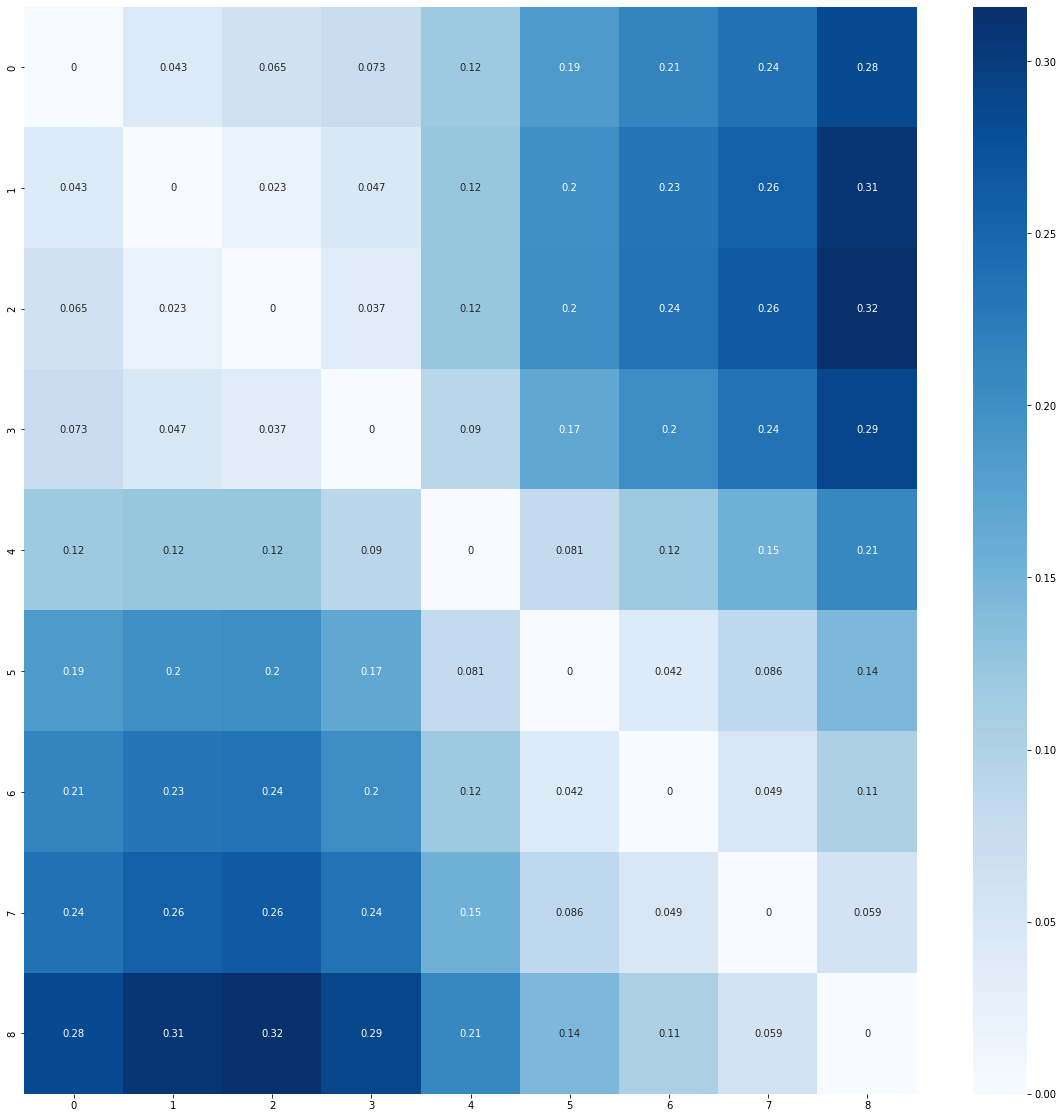
\includegraphics[width=7cm]{images/ordered_D.png} }}%
		\qquad
		\subfloat[\centering Kernel matrix depicted as heatmap label]{{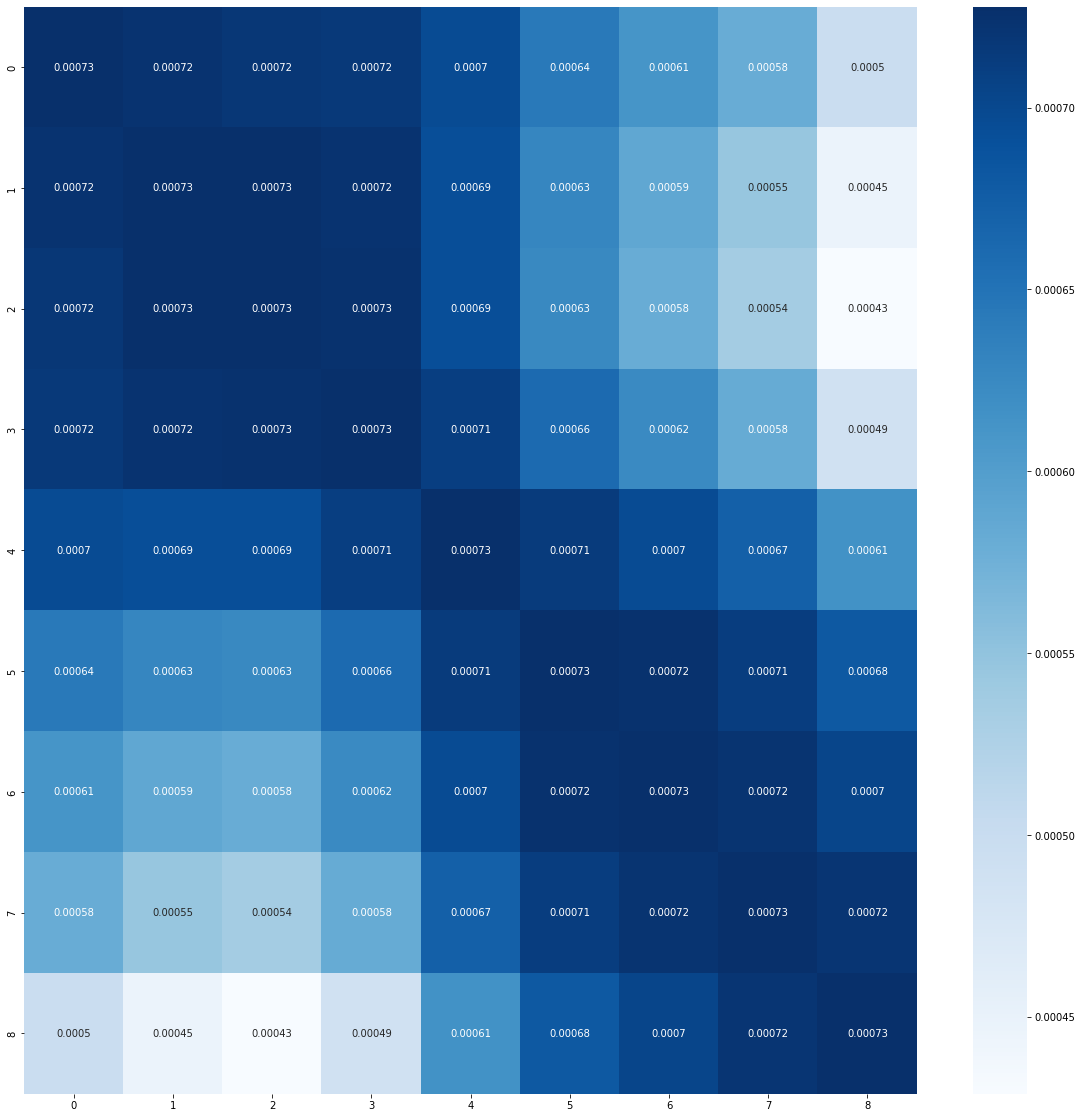
\includegraphics[width=7cm]{images/ordered_K.png} }}%
		\caption{Distance matrix and Kernel matrix for ordered set of images}%
		\label{fig:ordered_D_and_K}%
	\end{figure}
	
	\begin{figure}
		\centering
		\subfloat[\centering Distance matrix depicted as heatmap ]{{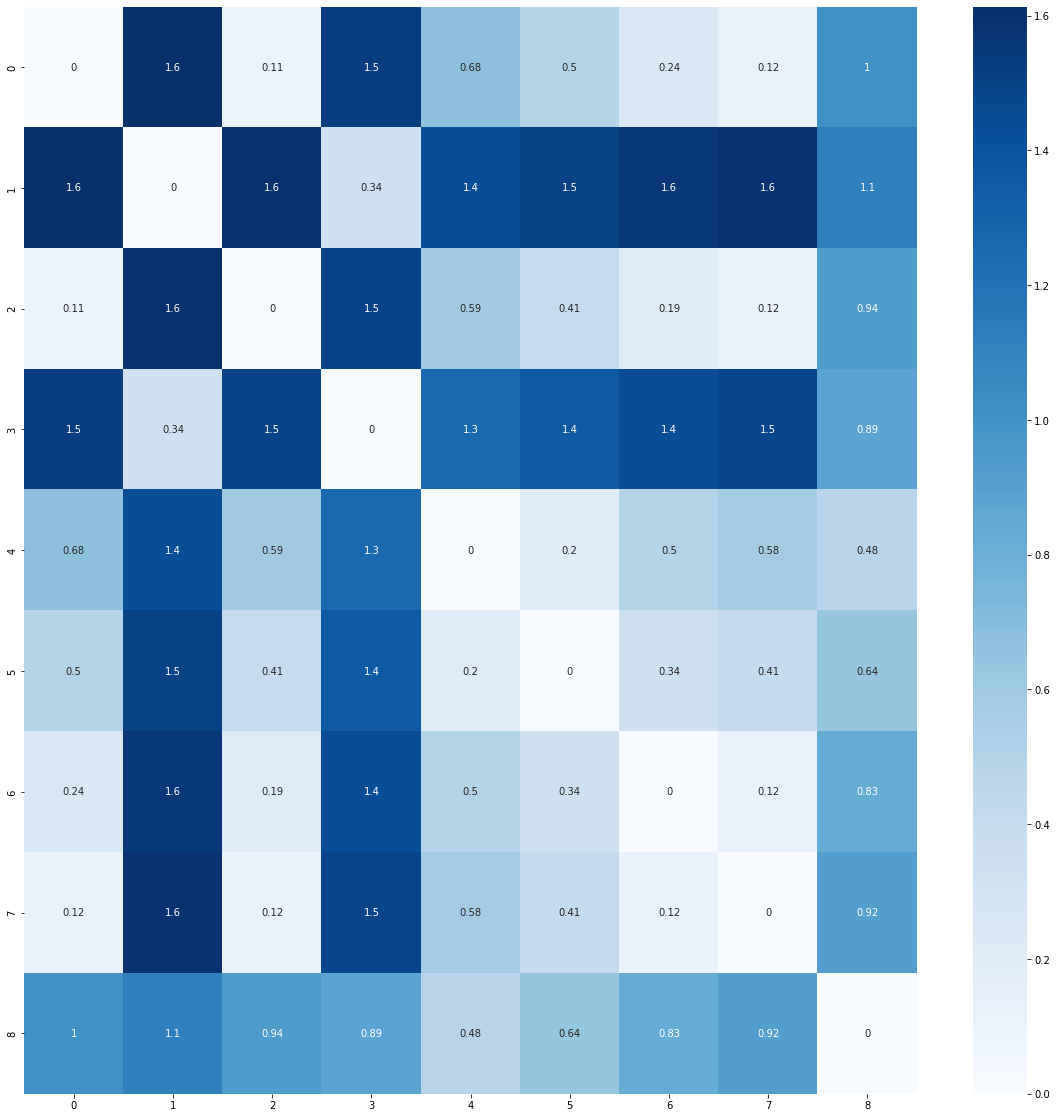
\includegraphics[width=7cm]{images/unordered_D.png} }}%
		\qquad
		\subfloat[\centering Kernel matrix depicted as heatmap 	label]{{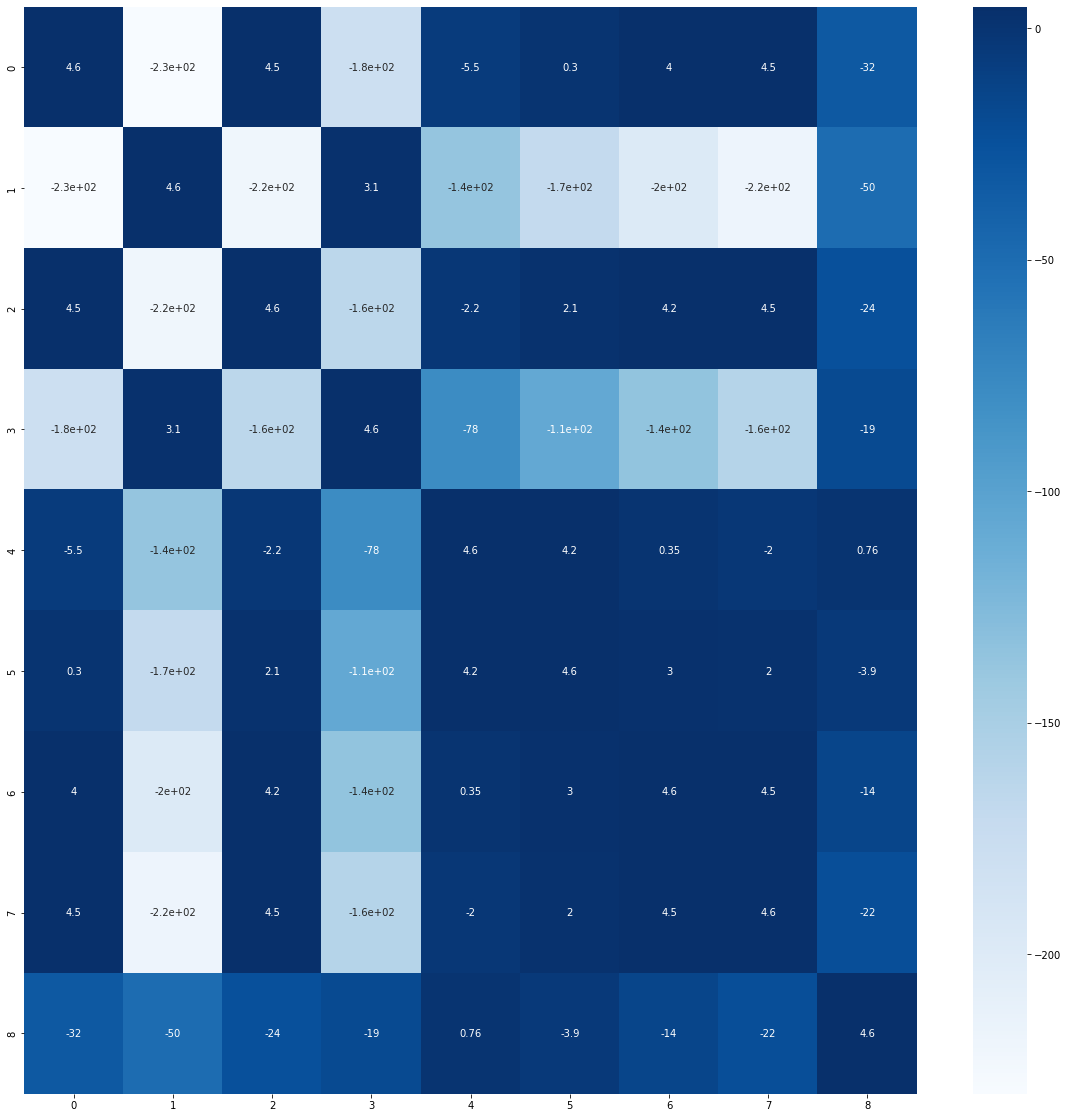
\includegraphics[width=7cm]{images/unordered_K.png} }}%
		\caption{Distance matrix and Kernel matrix for unordered set of images}%
		\label{fig:unordered_D_and_K}%
	\end{figure}
	
	%---------------------------------------------------------------------------------------------------------

    \subsection{Experiment1.1: U-Net Vanilla, GP and LSTM model considering all the classes}
    
    The below sections explain the results of the conducted experiments. The model is trained and tested with the scannet dataset without merging the classes. The model's performance is evaluated with Pixel accuracy, Mean pixel accuracy, meanIoU, IoU, and FwIoU metrics.

	%{ \bf Experiment1.1.1: U-Net vanilla model with all the classes}
	{ \bf Experiment1.1.2: U-Net vanilla model}
	
	The pixel accuracy is 50.96\% for the validation dataset. This is due to a large number of classes with unequal pixel distribution. However, the IoU for the Wall, Floor, and Mattress is high at 0.56, 0.608, and 0.382 due to the high pixel distribution for these classes. Frequency-weighted IoU considers the unequal pixel distribution, and the values stand at 0.3531. The predicted and the ground truth pixel distribution is presented in Fig \ref{fig:y_gt_pred_vanilla}. The bar plot shows that the predicted "Wall" class distribution is higher than the ground truth. The Wall and Floor class distribution is similar to the baseline and predicted class labels. 
    
    %------------------------------------------------------------------------------------------------------
   	
   	\begin{table}
    \begin{center}
    	\begin{tabular}{ | l | p{12cm} |}
    		\hline
    		
    		\cellcolor{purple!30}Metric & \cellcolor{purple!30}Value \\ \hline
    		Pixel Accuracy & 0.5096 \\ \hline
    		Pixel Mean accuracy & 0.1907  \\ \hline
    		meanIOU & 0.1102 \\ \hline
    		IoU & [1.8345e-01, 5.6047e-01, 6.0881e-01, 1.6476e-01, 3.8241e-01, 1.1697e-01, 
    		2.3122e-02, 8.9410e-02, 2.5848e-01, 1.6661e-01, 2.0180e-03, 2.0504e-01, 
    		4.5985e-02,        nan, 4.2167e-02, 1.1143e-01, 2.3969e-01, 1.2545e-02, 
    		1.1324e-01, 2.7658e-03, 0.0000e+00, 7.0415e-02, 7.0606e-02, 0.0000e+00,  
    		0.0000e+00, 1.2208e-01, 1.4680e-02, 1.1862e-04, 2.2112e-04, 6.5610e-03, 
    		4.3742e-03,        nan, 7.6680e-02, 3.5784e-02, 1.1516e-01, 5.6912e-02, 
    		2.9310e-04, 3.7764e-02, 2.2634e-02, 1.1269e-01, 2.2094e-01] \\ \hline
    		FwIoU & 0.3531 \\ \hline
    		\hline
    	\end{tabular}
   		\caption{A normal caption}
	    \label{tab:caption}
    \end{center}
	\end{table}

	\begin{figure}%
		\centering
		\subfloat[\centering Per class pixel distribution of the ground truth pixel class label ]{{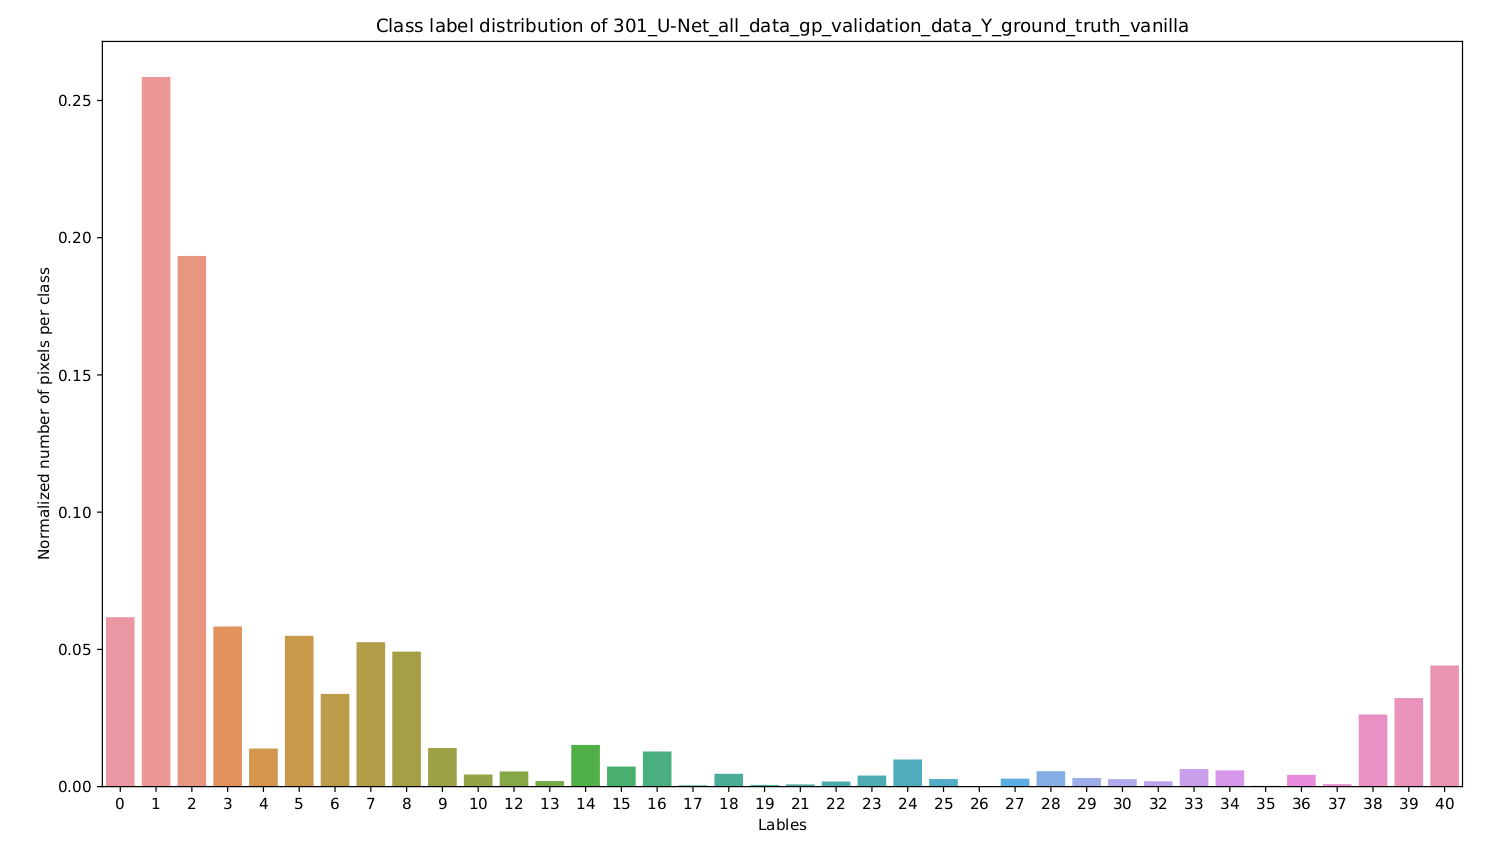
\includegraphics[width=7cm]{images/Y_ground_truth_vanilla.png} }}%
		\qquad
		\subfloat[\centering Per class pixel distribution of the predicted pixel class label]{{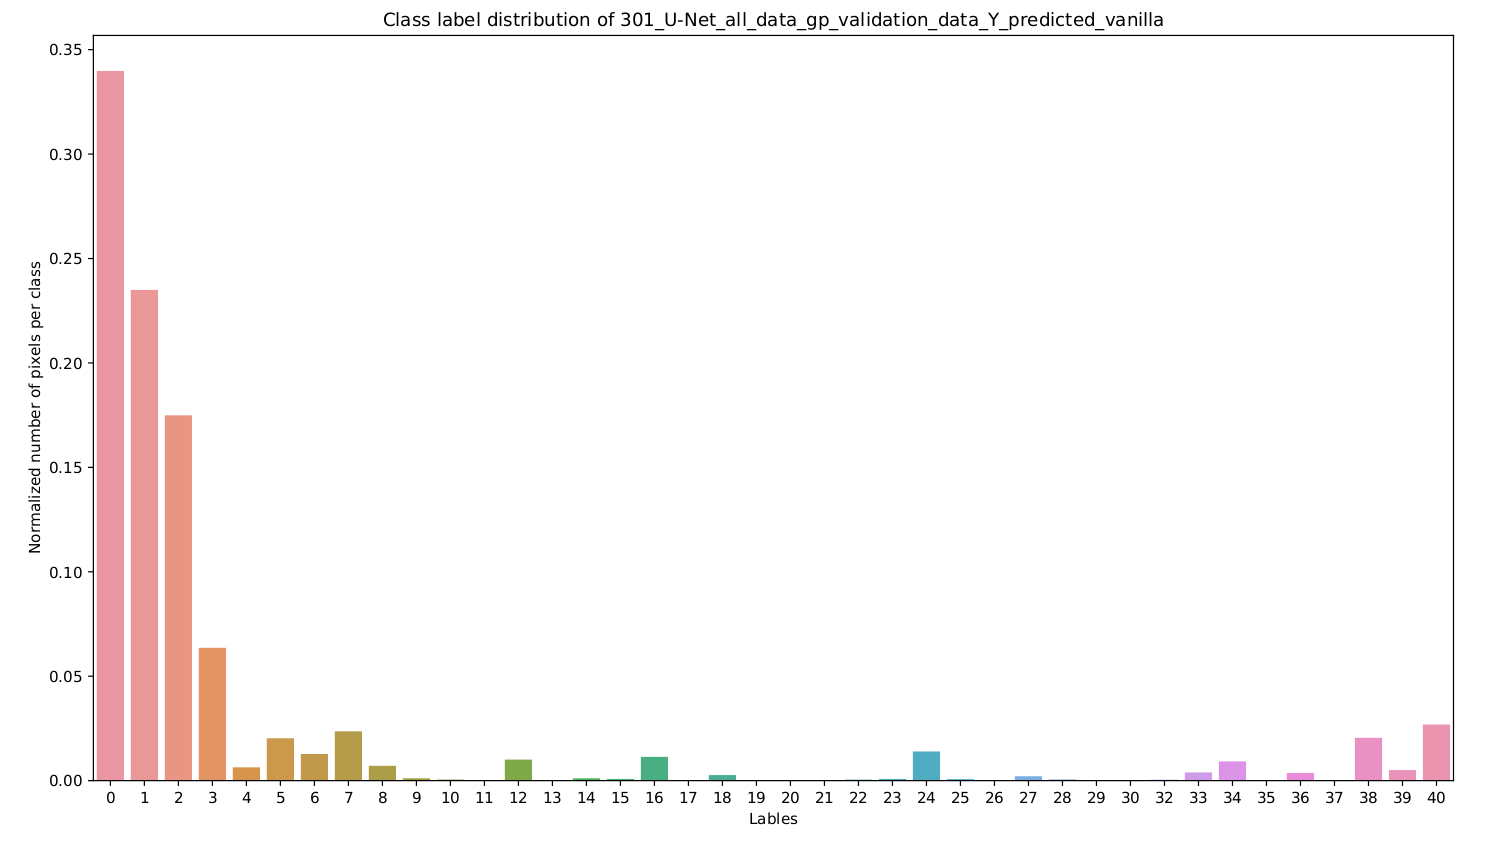
\includegraphics[width=7cm]{images/Y_predicted_vanilla.png} }}%
		\caption{Pixel distribution for the ground truth and predicted scannet data for vanilla unet model}%
		\label{fig:y_gt_pred_vanilla}%
	\end{figure}
    %------------------------------------------------------------------------------------------------------
    { \bf Experiment1.1.2: U-Net gp model}
    
    In the GP model experiment, the information from the previous frame is passed onto the current frame segmentation computation. The accuracy is slightly better than the vanilla model, with an increase of 1\% with the temporal fusion GP prior to integration. The latent space encoding is subjected to the Gaussian process and then passed onto the decoder for segmentation computation. The mean pixel accuracy is similar to the vanilla model, with slight improvement. A large number of classes is causing the drop in performance. As expected "Wall," "Floor," and "Furniture" classes have high IoU values due to the presence of high pixel distribution. 
    
    \begin{table}
	\begin{center}
		\begin{tabular}{ | l | p{12cm} |}
			\hline
			
			\cellcolor{purple!30}Metric & \cellcolor{purple!30}Value \\ \hline
			Pixel Accuracy & 0.5184 \\ \hline
			Pixel Mean accuracy & 0.1679  \\ \hline
			meanIOU & 0.1161 \\ \hline
			IoU & [1.7087e-01, 5.1271e-01, 5.9998e-01, 2.1256e-01, 4.1160e-01, 1.5834e-01,
			3.8634e-02, 2.3669e-01, 1.6056e-01, 1.1568e-01, 7.9677e-02, 1.0454e-02,
			2.4003e-02, 0.0000e+00, 1.2199e-01, 4.3193e-02, 3.3956e-01, 6.6473e-02,
			1.4712e-01, 2.8003e-03, 6.0475e-05, 2.6127e-01, 5.7962e-02, 0.0000e+00,
			3.4611e-04, 1.6519e-02, 0.0000e+00, 4.3417e-04, 4.4221e-02, 6.6478e-03,
			1.2108e-02,        nan, 5.3272e-02, 5.8480e-02, 2.2352e-01, 4.2175e-02,
			8.4644e-02, 1.1630e-04, 4.9106e-02, 1.0338e-01, 1.7687e-01] \\ \hline
			FwIoU & 0.3497 \\ \hline
			\hline
		\end{tabular}
		\caption{A normal caption}
		\label{tab:caption}
	\end{center}
	\end{table}
	
	\begin{figure}%
		\centering
		\subfloat[\centering Per class pixel distribution of the ground truth pixel class label for gp model ]{{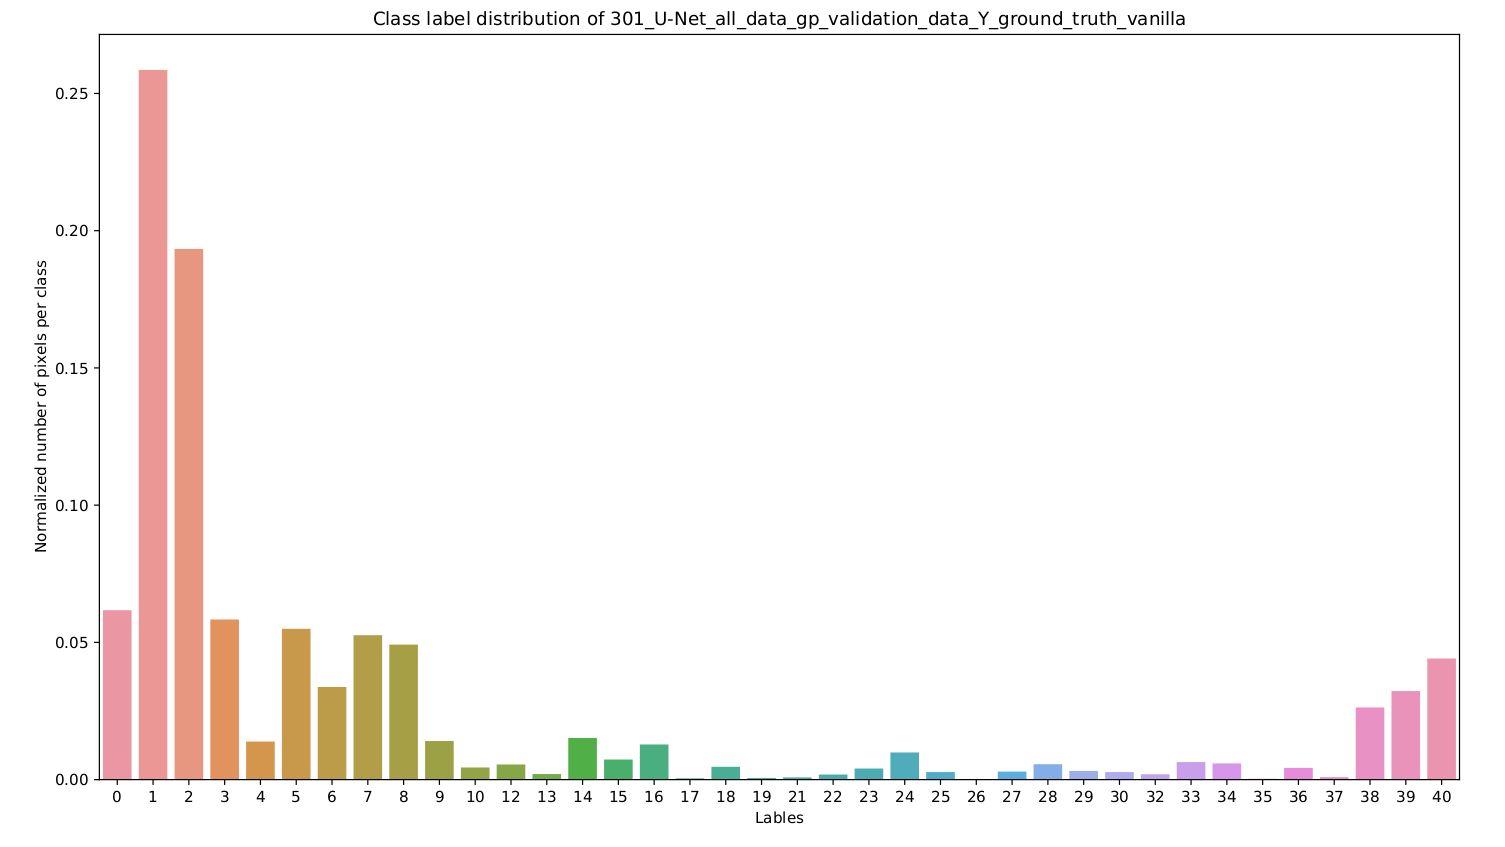
\includegraphics[width=7cm]{images/Y_ground_truth_gp.png} }}%
		\qquad
		\subfloat[\centering Per class pixel distribution of the predicted pixel class for gp model 	label]{{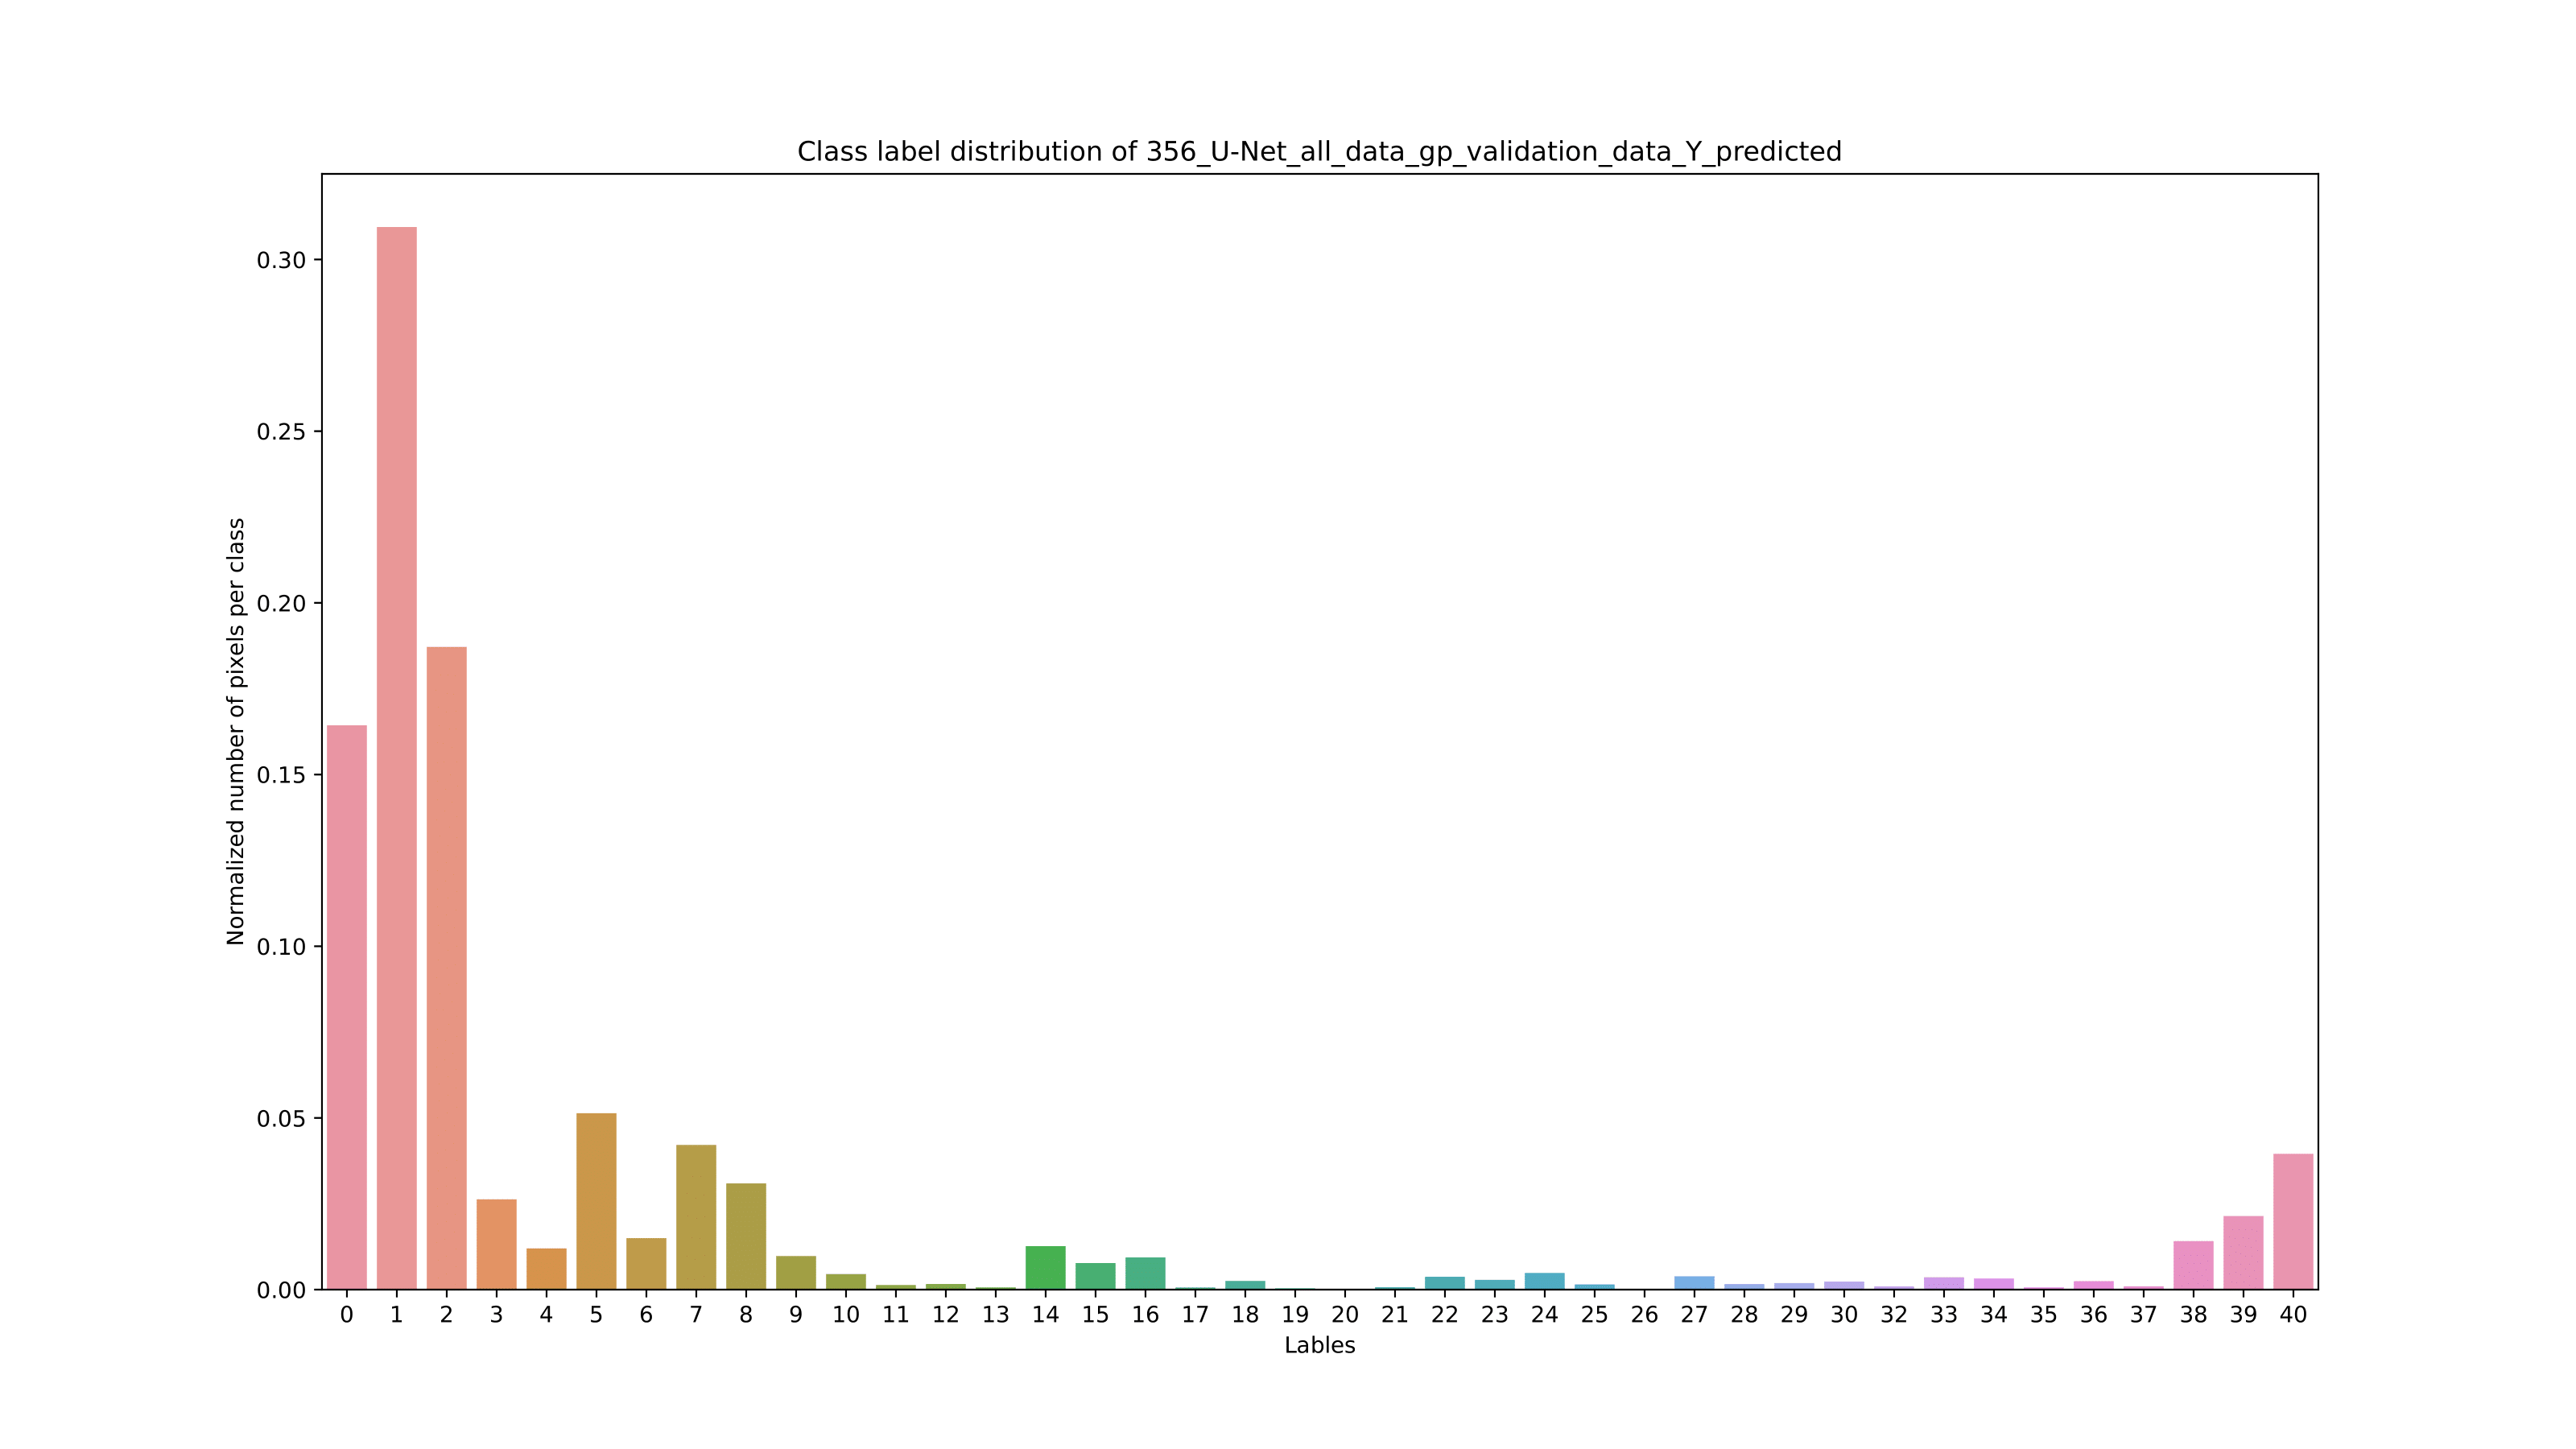
\includegraphics[width=7cm]{images/Y_predicted_gp.png} }}%
		\caption{Per class pixel distribution of the predicted pixel class label for gp model}%
		\label{fig:y_gt_and_predic_gp}%
	\end{figure}

    %------------------------------------------------------------------------------------------------------
    \newpage
	{ \bf Experiment1.1.2: U-Net lstm model}
	
	The scene geometry from the past frame is passed onto a current frame efficiently with the lstm model. The ConvLSTM cell at the latent space compress and store the past information in its states. The change in the viewpoint is captured by the hidden state and passed onto the next hidden state for the computation of the segmentation map. From the result table \ref{tab:lstm_result_all_classes}, it is evident that the accuracy has improved by 6\% and 5\% in comparison with the vanilla and GP models, respectively. Mean accuracy has increased by quite a significant margin. A large margin also improves the IoU values. IoU for the "Wall" class is highest with 0.61 in comparison with the vanilla and GP approach. However, for the cabinet class, GP performed well. Table, bookshelf, Counter, and desk class GP outperformed the vanilla and LSTM model. 
	
	\begin{table}
	\begin{center}
		\begin{tabular}{ | l | p{12cm} |}
			\hline		
			\cellcolor{purple!30}Metric & \cellcolor{purple!30}Value \\ \hline
			Pixel Accuracy & 0.5426 \\ \hline
			Pixel Mean accuracy & 0.3509  \\ \hline
			meanIOU & 0.1411 \\ \hline
			IoU & [0.1690, 0.5573, 0.5949, 0.1428, 0.1170, 0.1984, 0.1930, 0.1278, 0.2010,
			0.0778, 0.0071, 0.0514, 0.0216, 0.0070, 0.0426, 0.0610, 0.1063, 0.0020,
			0.0907, 0.0017, 0.0000, 0.0114, 0.0422, 0.0015, 0.0380, 0.0209, 0.0000,
			0.0362, 0.0710, 0.0010, 0.0182, 0.0000, 0.0174, 0.1382, 0.0534, 0.0077,
			0.0558, 0.0016, 0.0646, 0.1776, 0.1697] \\ \hline
			FwIoU & 0.7643 \\ \hline
			\hline
		\end{tabular}
		\caption{A normal caption}
		\label{tab:caption}
	\end{center}
	\end{table}
	
	\begin{figure}%
		\centering
		\subfloat[\centering Per class pixel distribution of the ground truth pixel class label for lstm model ]{{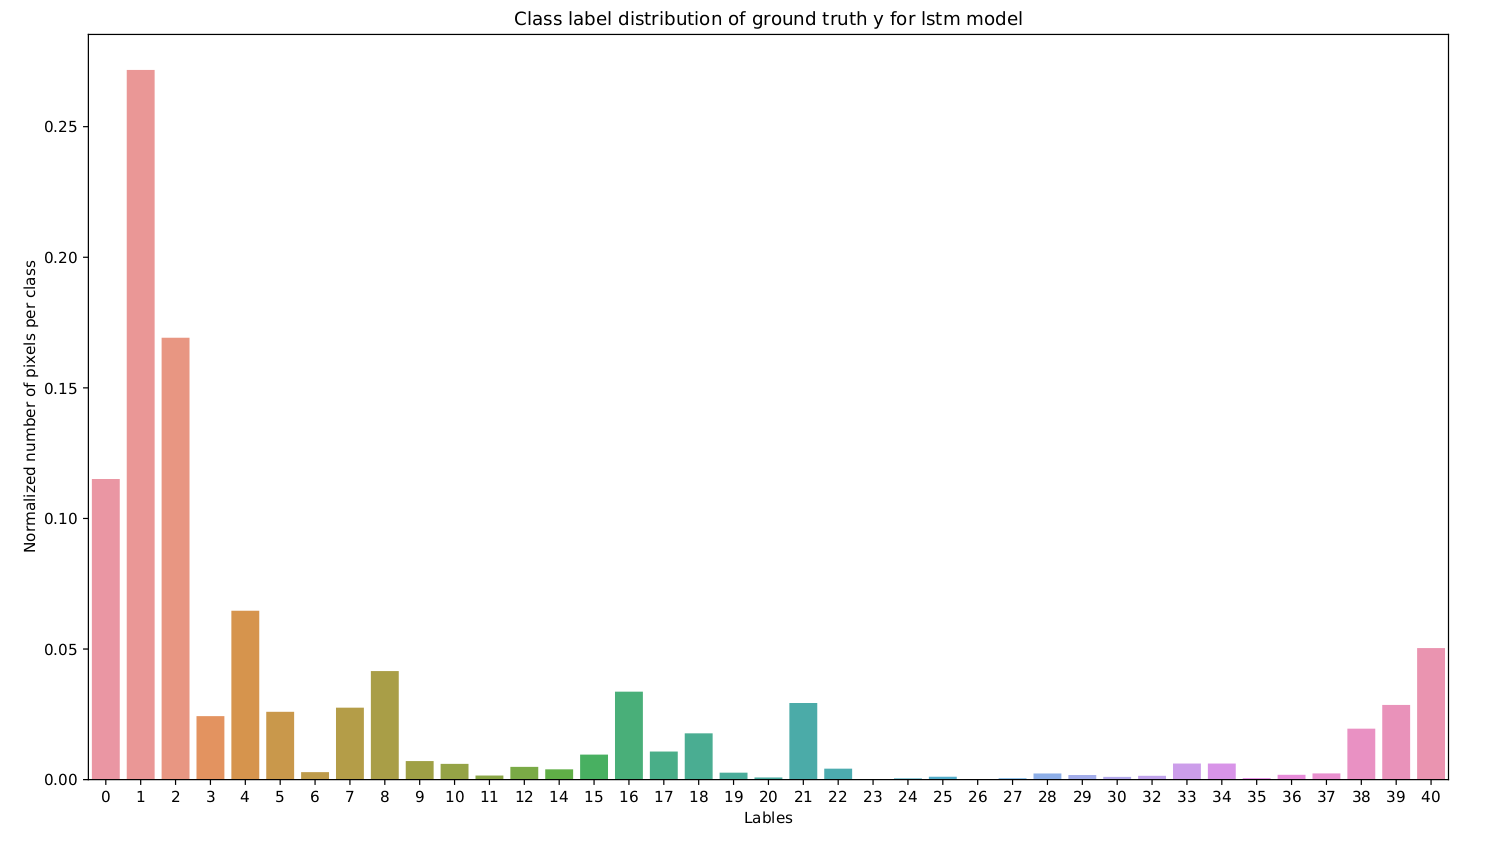
\includegraphics[width=7cm]{images/Y_ground_truth_lstm.png} }}%
		\qquad
		\subfloat[\centering Per class pixel distribution of the predicted pixel class for lstm model]{{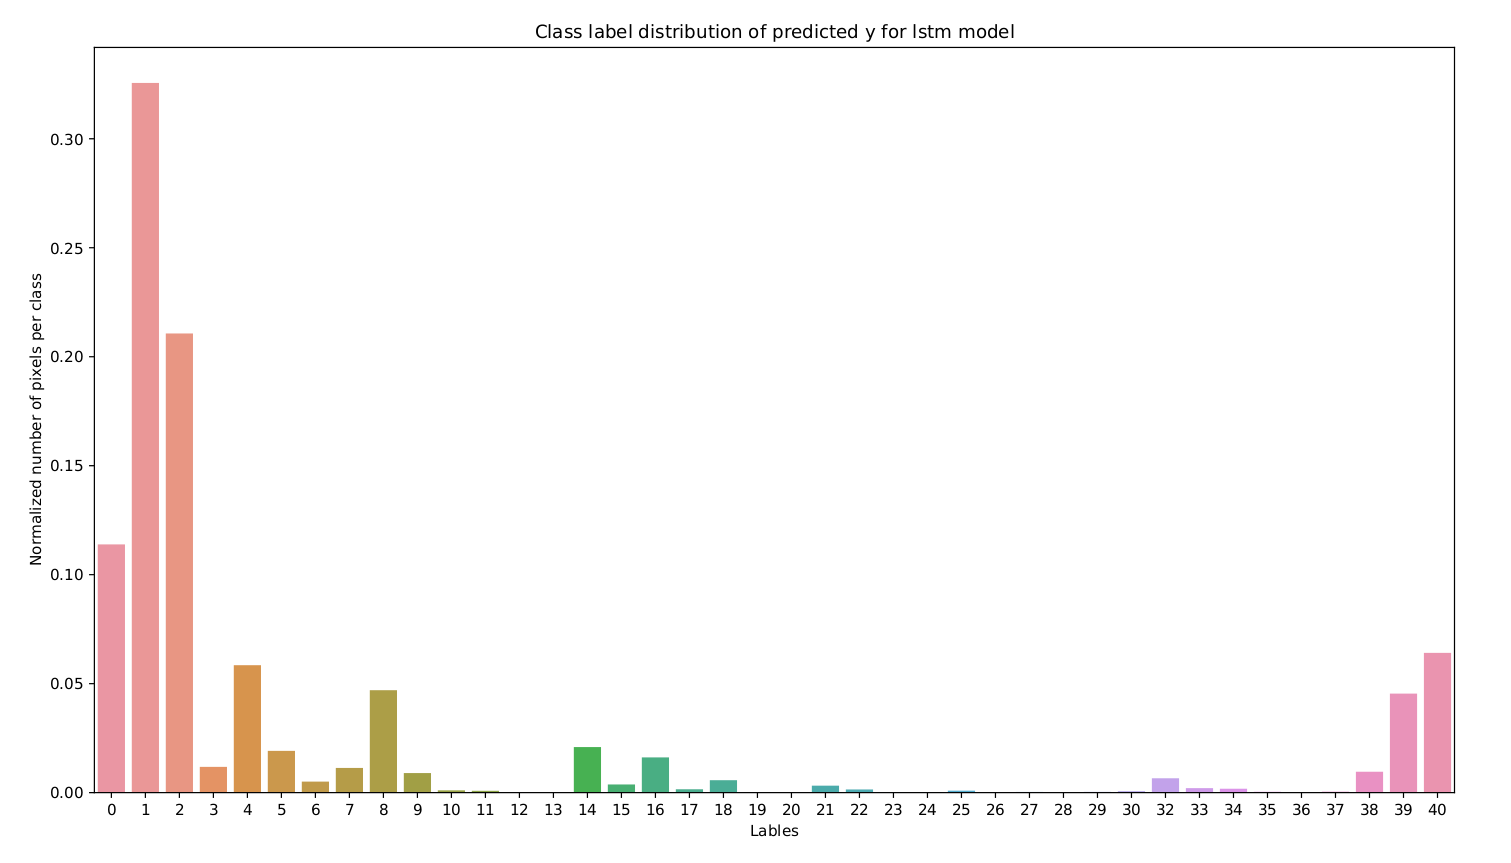
\includegraphics[width=7cm]{images/Y_predicted_lstm.png} }}%
		\caption{Per class pixel distribution of the predicted pixel class label for lstm model}%
		\label{fig:y_gt_and_predic_lstm}%
	\end{figure}

	Accuracy, mean accuracy, meanIoU, and FWIoU comparison is plotted as the bar graph in \ref{fig:unet_model_metric_comparison_all_classes}. The accuracy is highest for the LSTM model compared to the vanilla and GP. However, the mean accuracy is lowest for the GP model concerning other models. The experiment shows that the performance improves by incorporating temporal fusion in the semantic segmentation for the continuous sequence data. The overlapping and the past information is learned, stored, and passed onto the computation of the future frames' semantic segmentation. The temporal dependency between the frames is exploited to efficiently perform the segmentation by taking pose into account in the Gaussian process and compressed information in the hidden state of the ConVlstm cell. The Gaussian process works because if the two frames are very close to each other, represented by the pose information, there is a high probability of overlapping regions in the consecutive frames. The output of the decoder is based on the input to the decoder. The output of the encoder is passed onto the gaussian process; it takes into account the current and previous pose information and outputs a latent encoding based on the distance between the current and the previous frame. Hence, if two frames are close to each other, then the latent output of the Gaussian process is similar, resulting in information transfer from the past learned latent representation to the current latent output resulting in improved performance. The raw RGB ground truth and predicted segmentation map are compared in Fig \ref{fig:unet_model}. It can be observed from the figure that the Vanilla and LSTM model performed reasonably well in comparison with the GP model. However, overall metric-wise, LSTM outperformed vanilla and GP.   
	
	\begin{figure}
		\centering
		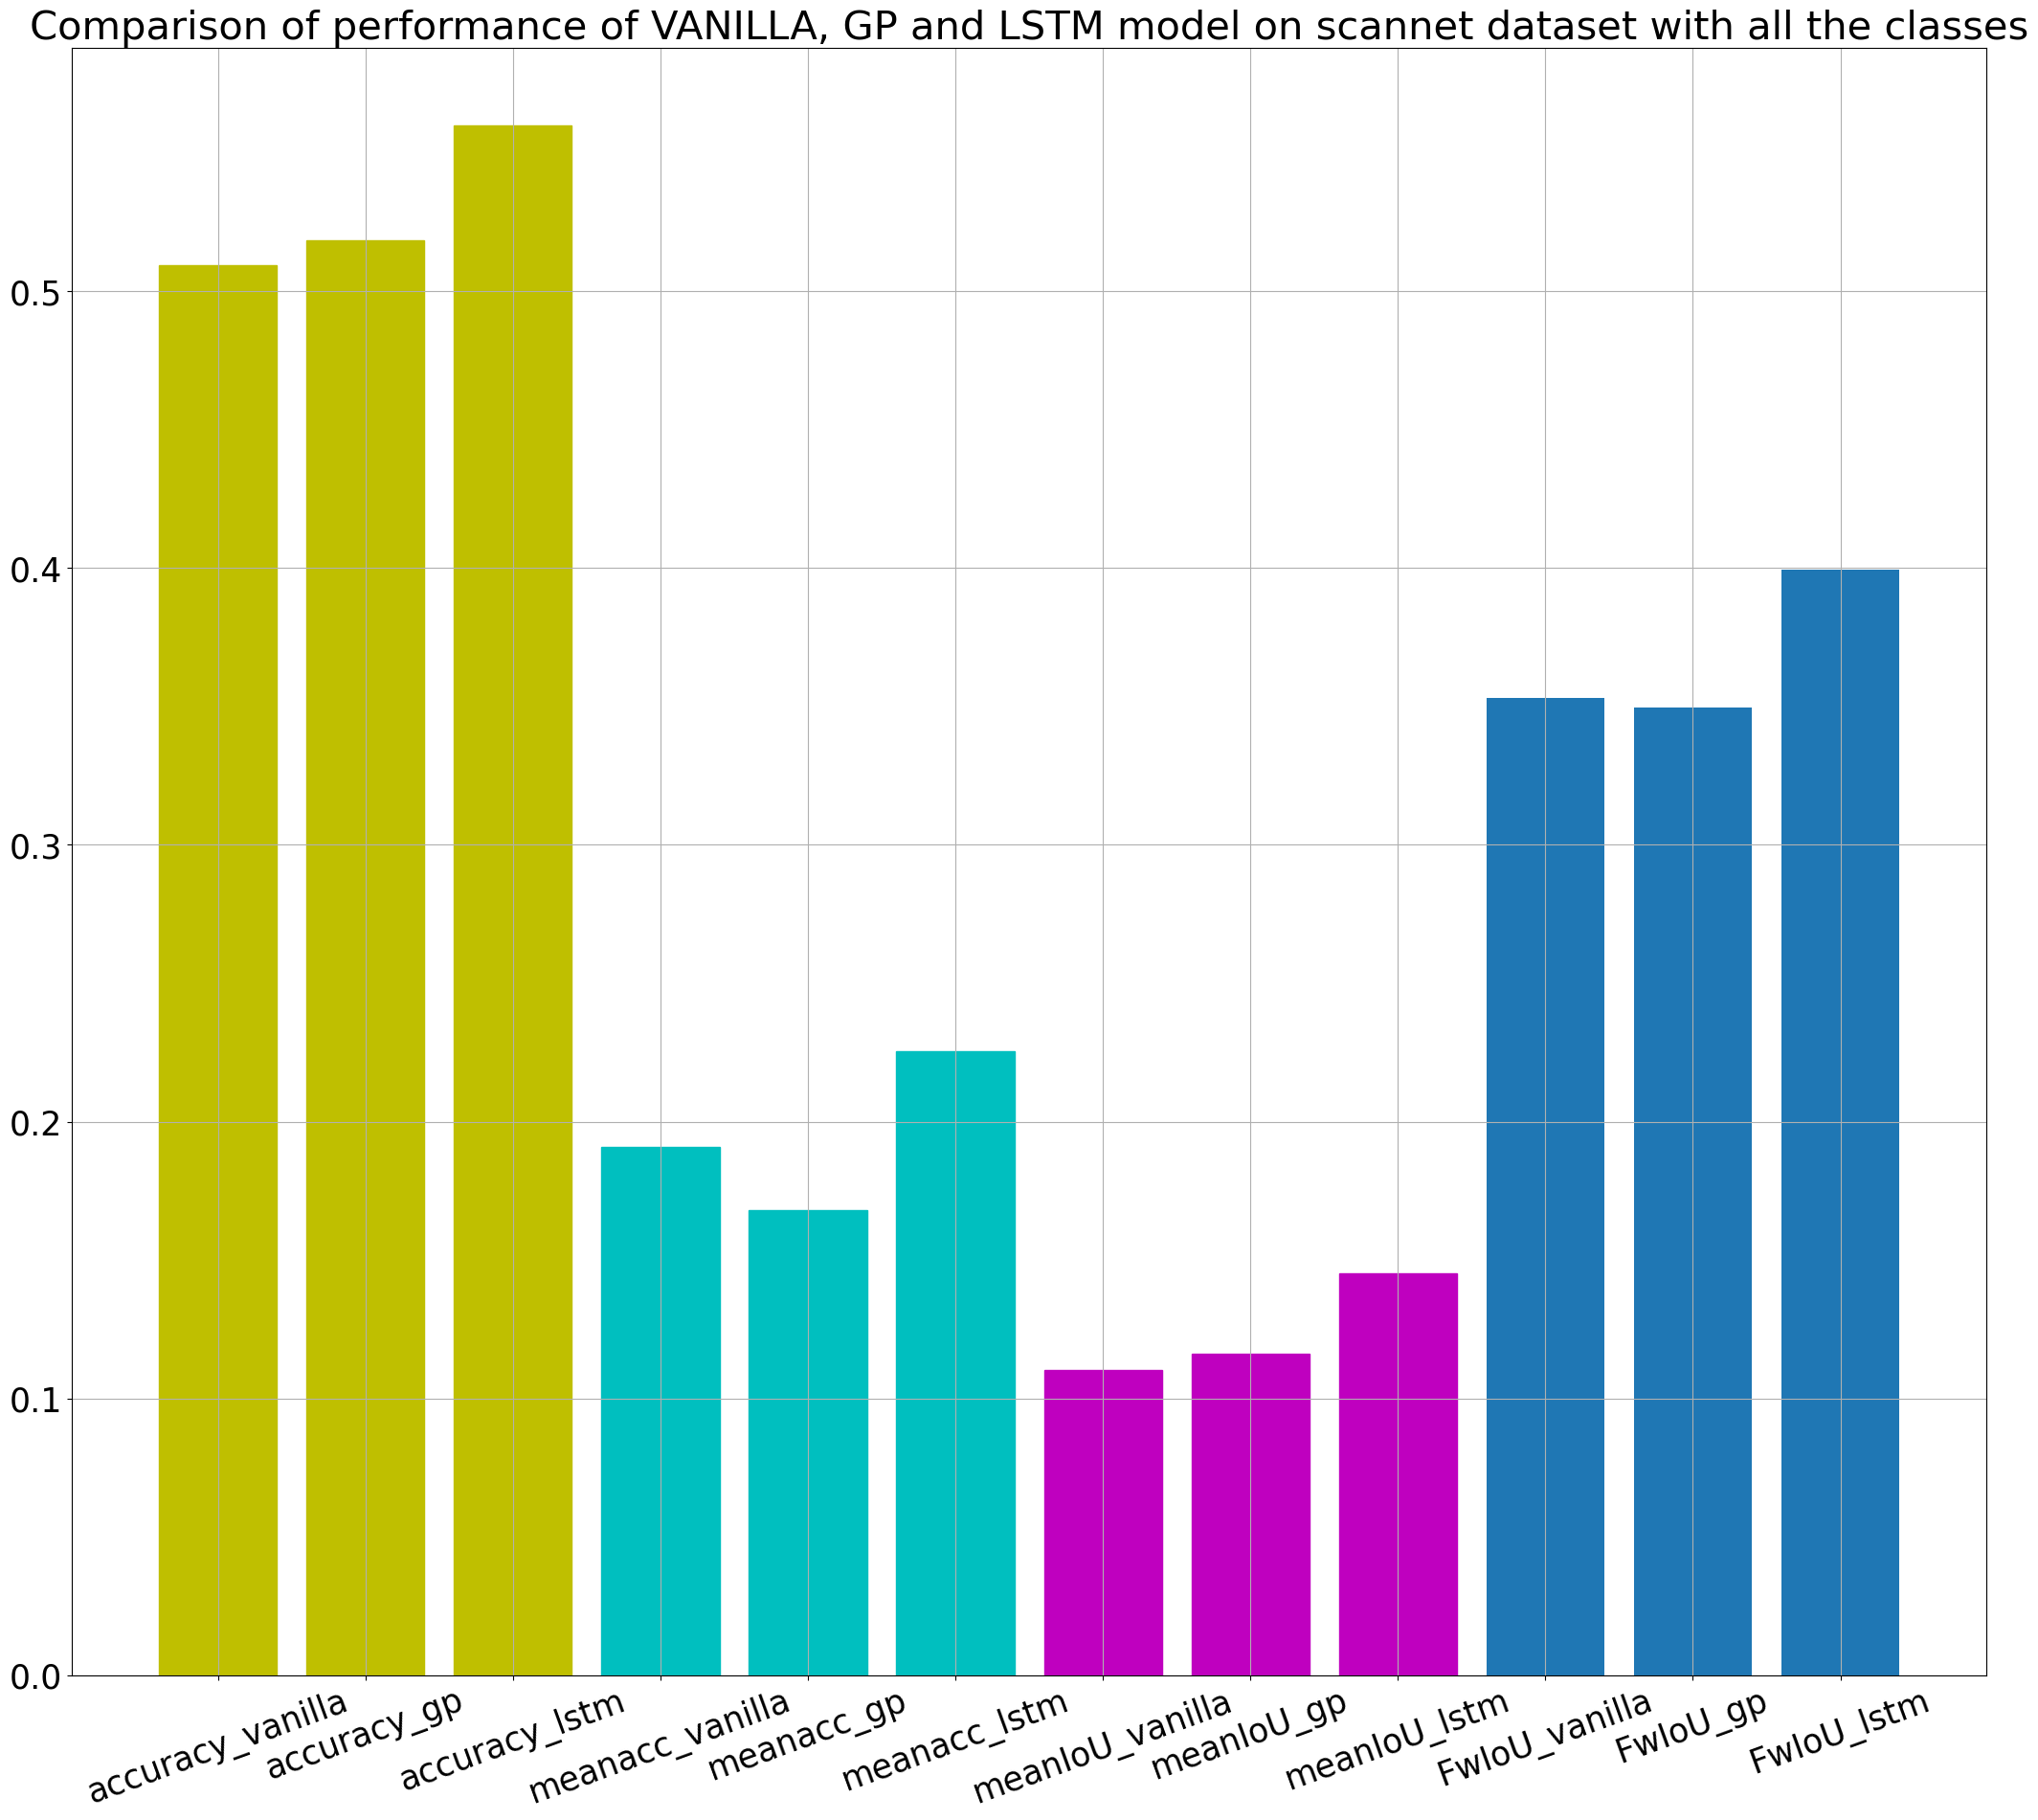
\includegraphics[width=12cm]{images/scannet_performance_all_classes.png}
		\caption{Comparison of VANILLA, GP and LSTM model performance based on metric}
		\label{fig:unet_model_metric_comparison_all_classes}
	\end{figure}
	
	\begin{figure}
		\centering
		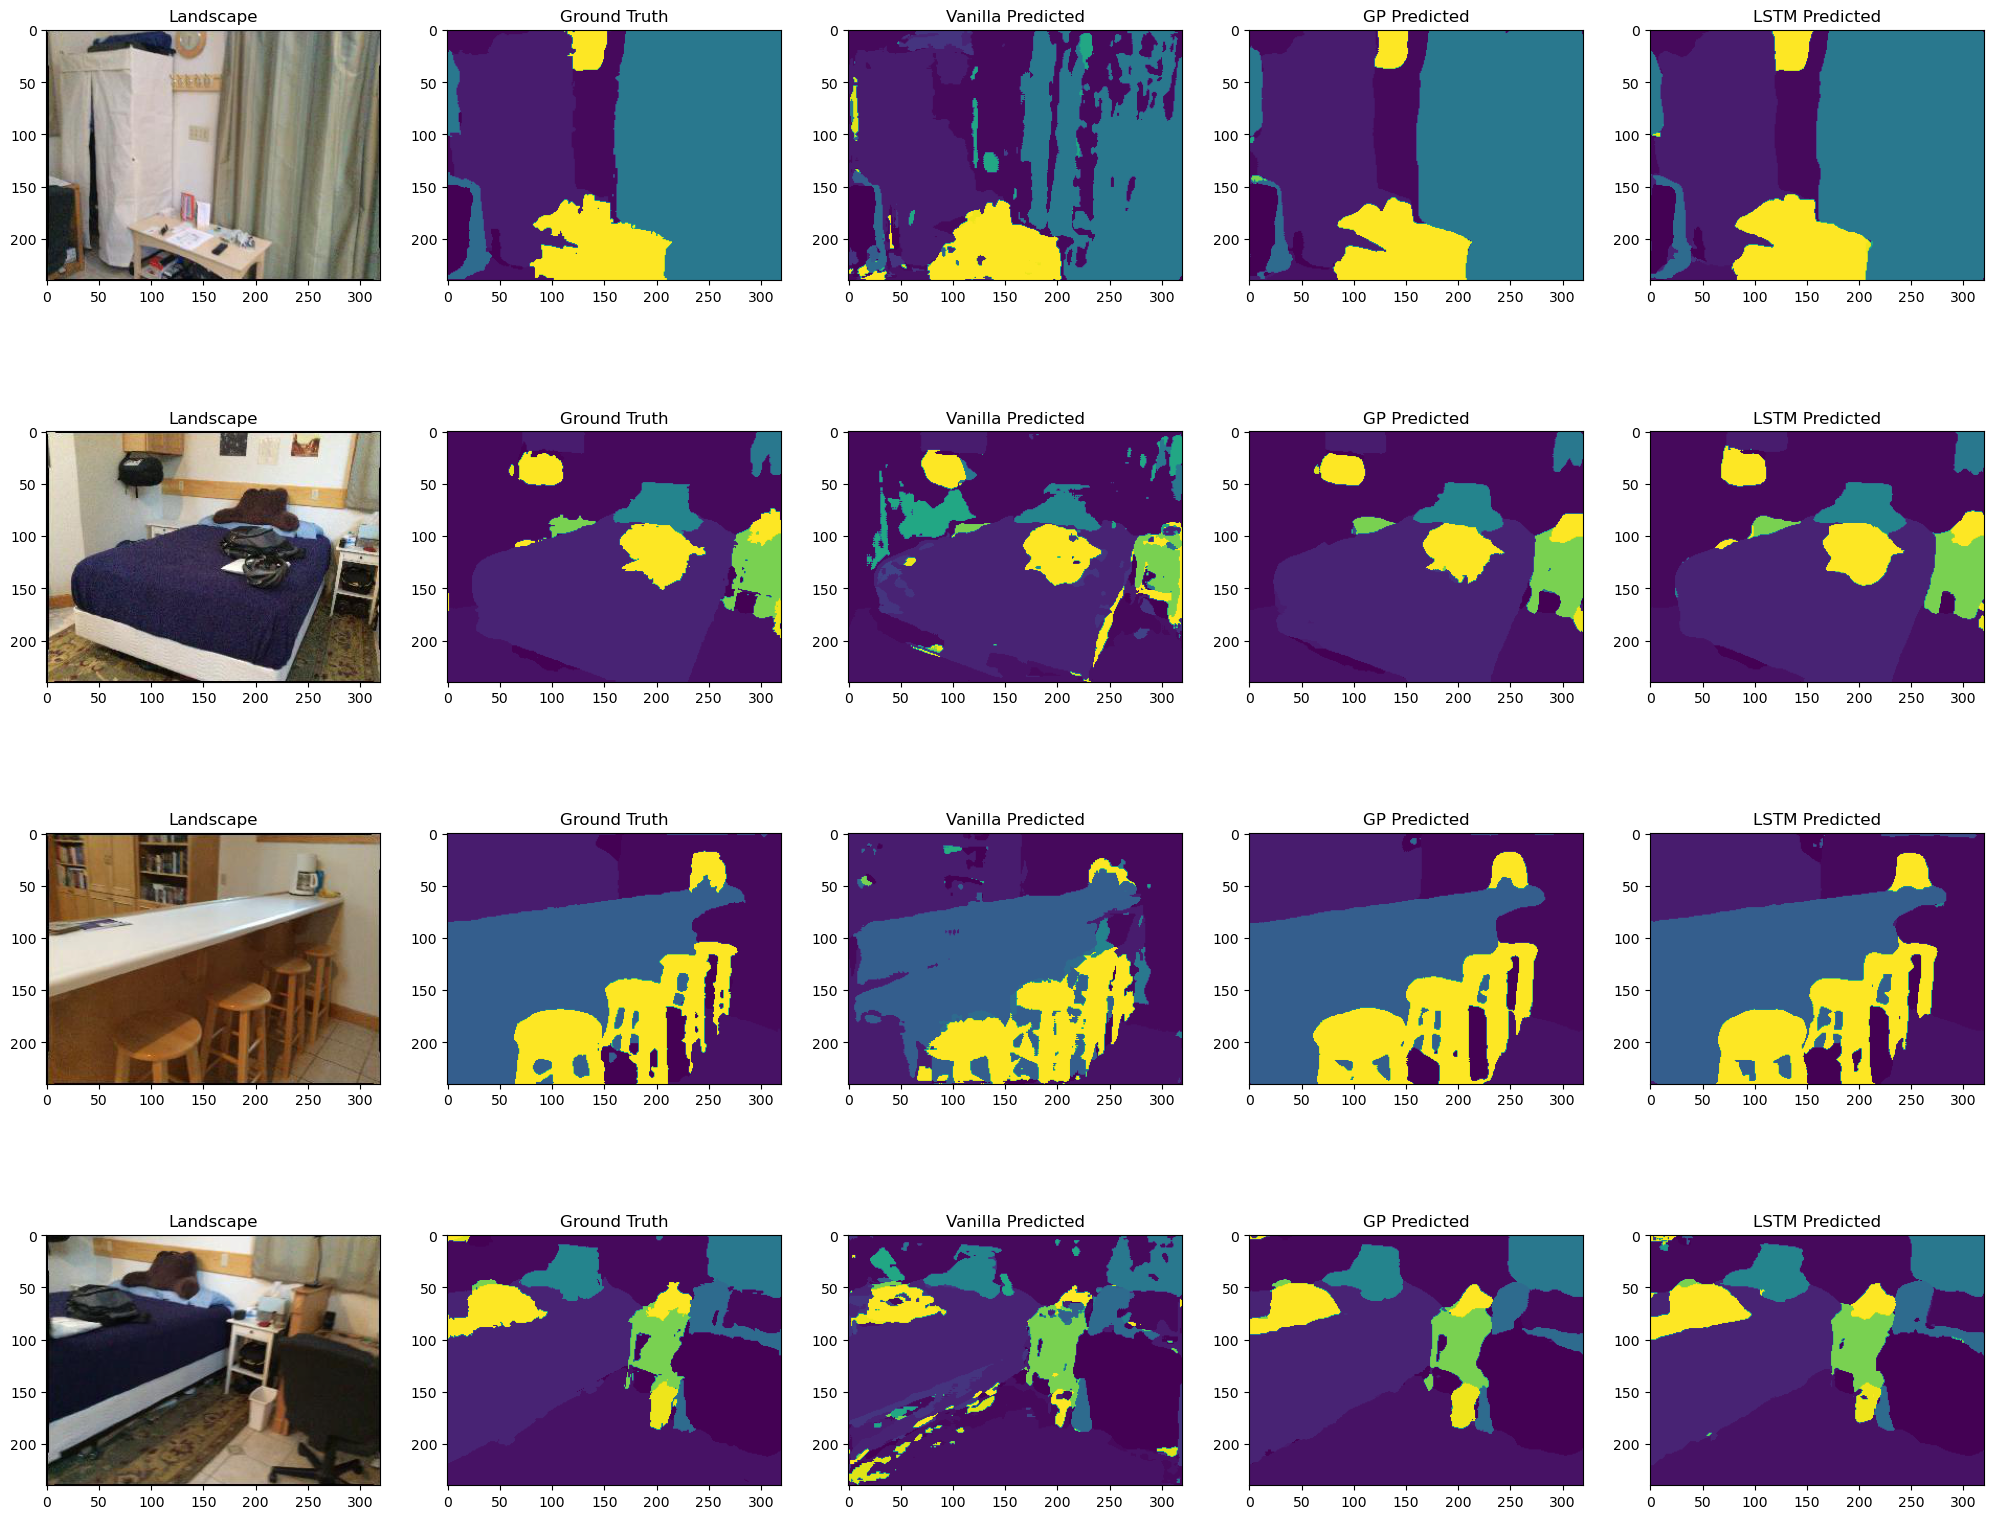
\includegraphics[width=16cm]{images/unet_scannet_all_classes.png}
		\caption{Plotting of raw input image, ground truth and predicted output for vanilla, gp and lstm model}
		\label{fig:unet_model}
	\end{figure}

	\newpage
		
    \subsection{Experiment1.2: U-Net Vanilla, Temporally fused gp model and LSTM model considering two classes}
    %------------------------------------------------------------------------------------------------------
	In the second experiment on the scannet dataset, all the classes are combined except the wall class resulting in the wall and other classes. Table \ref{table:unet_two_classes} compares the results of vanilla, GP, and LSTM model performance. In this case, the pixel accuracy is similar in the vanilla and the lstm model; however, the accuracy dropped for the GP model. A similar observation can be made with the mean accuracy. However, the meanIoU value is high for the lstm model at 0.28, and vanilla and GP produced a result of 0.14 and 0.23. The frequency-weighted intersection over union is high for the lstm model, followed by the vanilla and GP model. A comparison of model output is presented in Fig \ref{fig:output_vanilla}. In this case, the wall and other categories in the test image are segmented reasonably well by the LSTM model. The metric bar comparison is shown in Fig \ref{fig:unet_model_metric_comparison}. It is evident from the plot that the mean accuracy is good for the vanilla and GP and lstm performance is below the other models. However, the meanIoU and FWIoU are high for the lstm model.

	\begin{figure}[h]
		\centering
		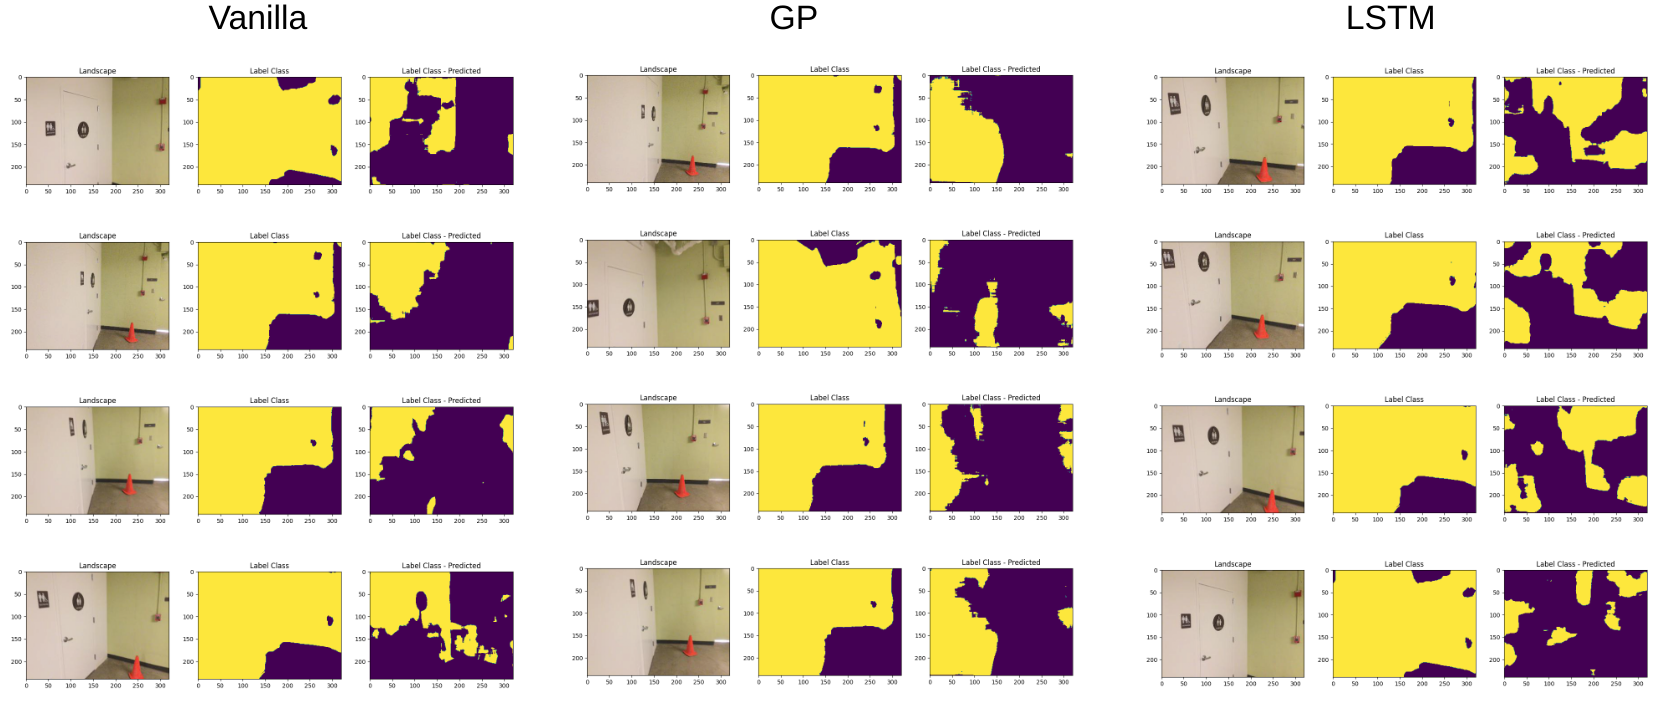
\includegraphics[width=16cm]{images/output_unet_two_classes.png}
		\caption{Plotting of raw input image, ground truth and predicted output for vanilla, gp and lstm model for two class dataset}
		\label{fig:output_vanilla}
	\end{figure}
	
	\begin{table}[h]
		\begin{center}
			\begin{tabular}{ | l | l | l | p{4cm} |}
				\hline
				
				\cellcolor{purple!30}Metric & \cellcolor{purple!30}Vanilla & \cellcolor{purple!30}GP & \cellcolor{purple!30}LSTM\\ \hline
				Pixel Accuracy & 0.4342 & 0.3764 & 0.8549\\ \hline
				Pixel Mean accuracy & 0.6232 & 0.5625 & 0.7837 \\ \hline
				meanIOU & 0.145 & 0.2318 & 0.6593 \\ \hline
				IoU & [0.2737, 0.2809] & [0.2377, 0.2259] & [0.8280, 0.4903] \\ \hline
				FwIoU & 0.2793 & 0.2284 & 0.7643 \\ \hline
				\hline
			\end{tabular}
			\caption{Performance of Vanilla model with respect to different metric and two classes}
			\label{table:unet_two_classes}
		\end{center}
	\end{table}
	
	
	\begin{figure}
		\centering
		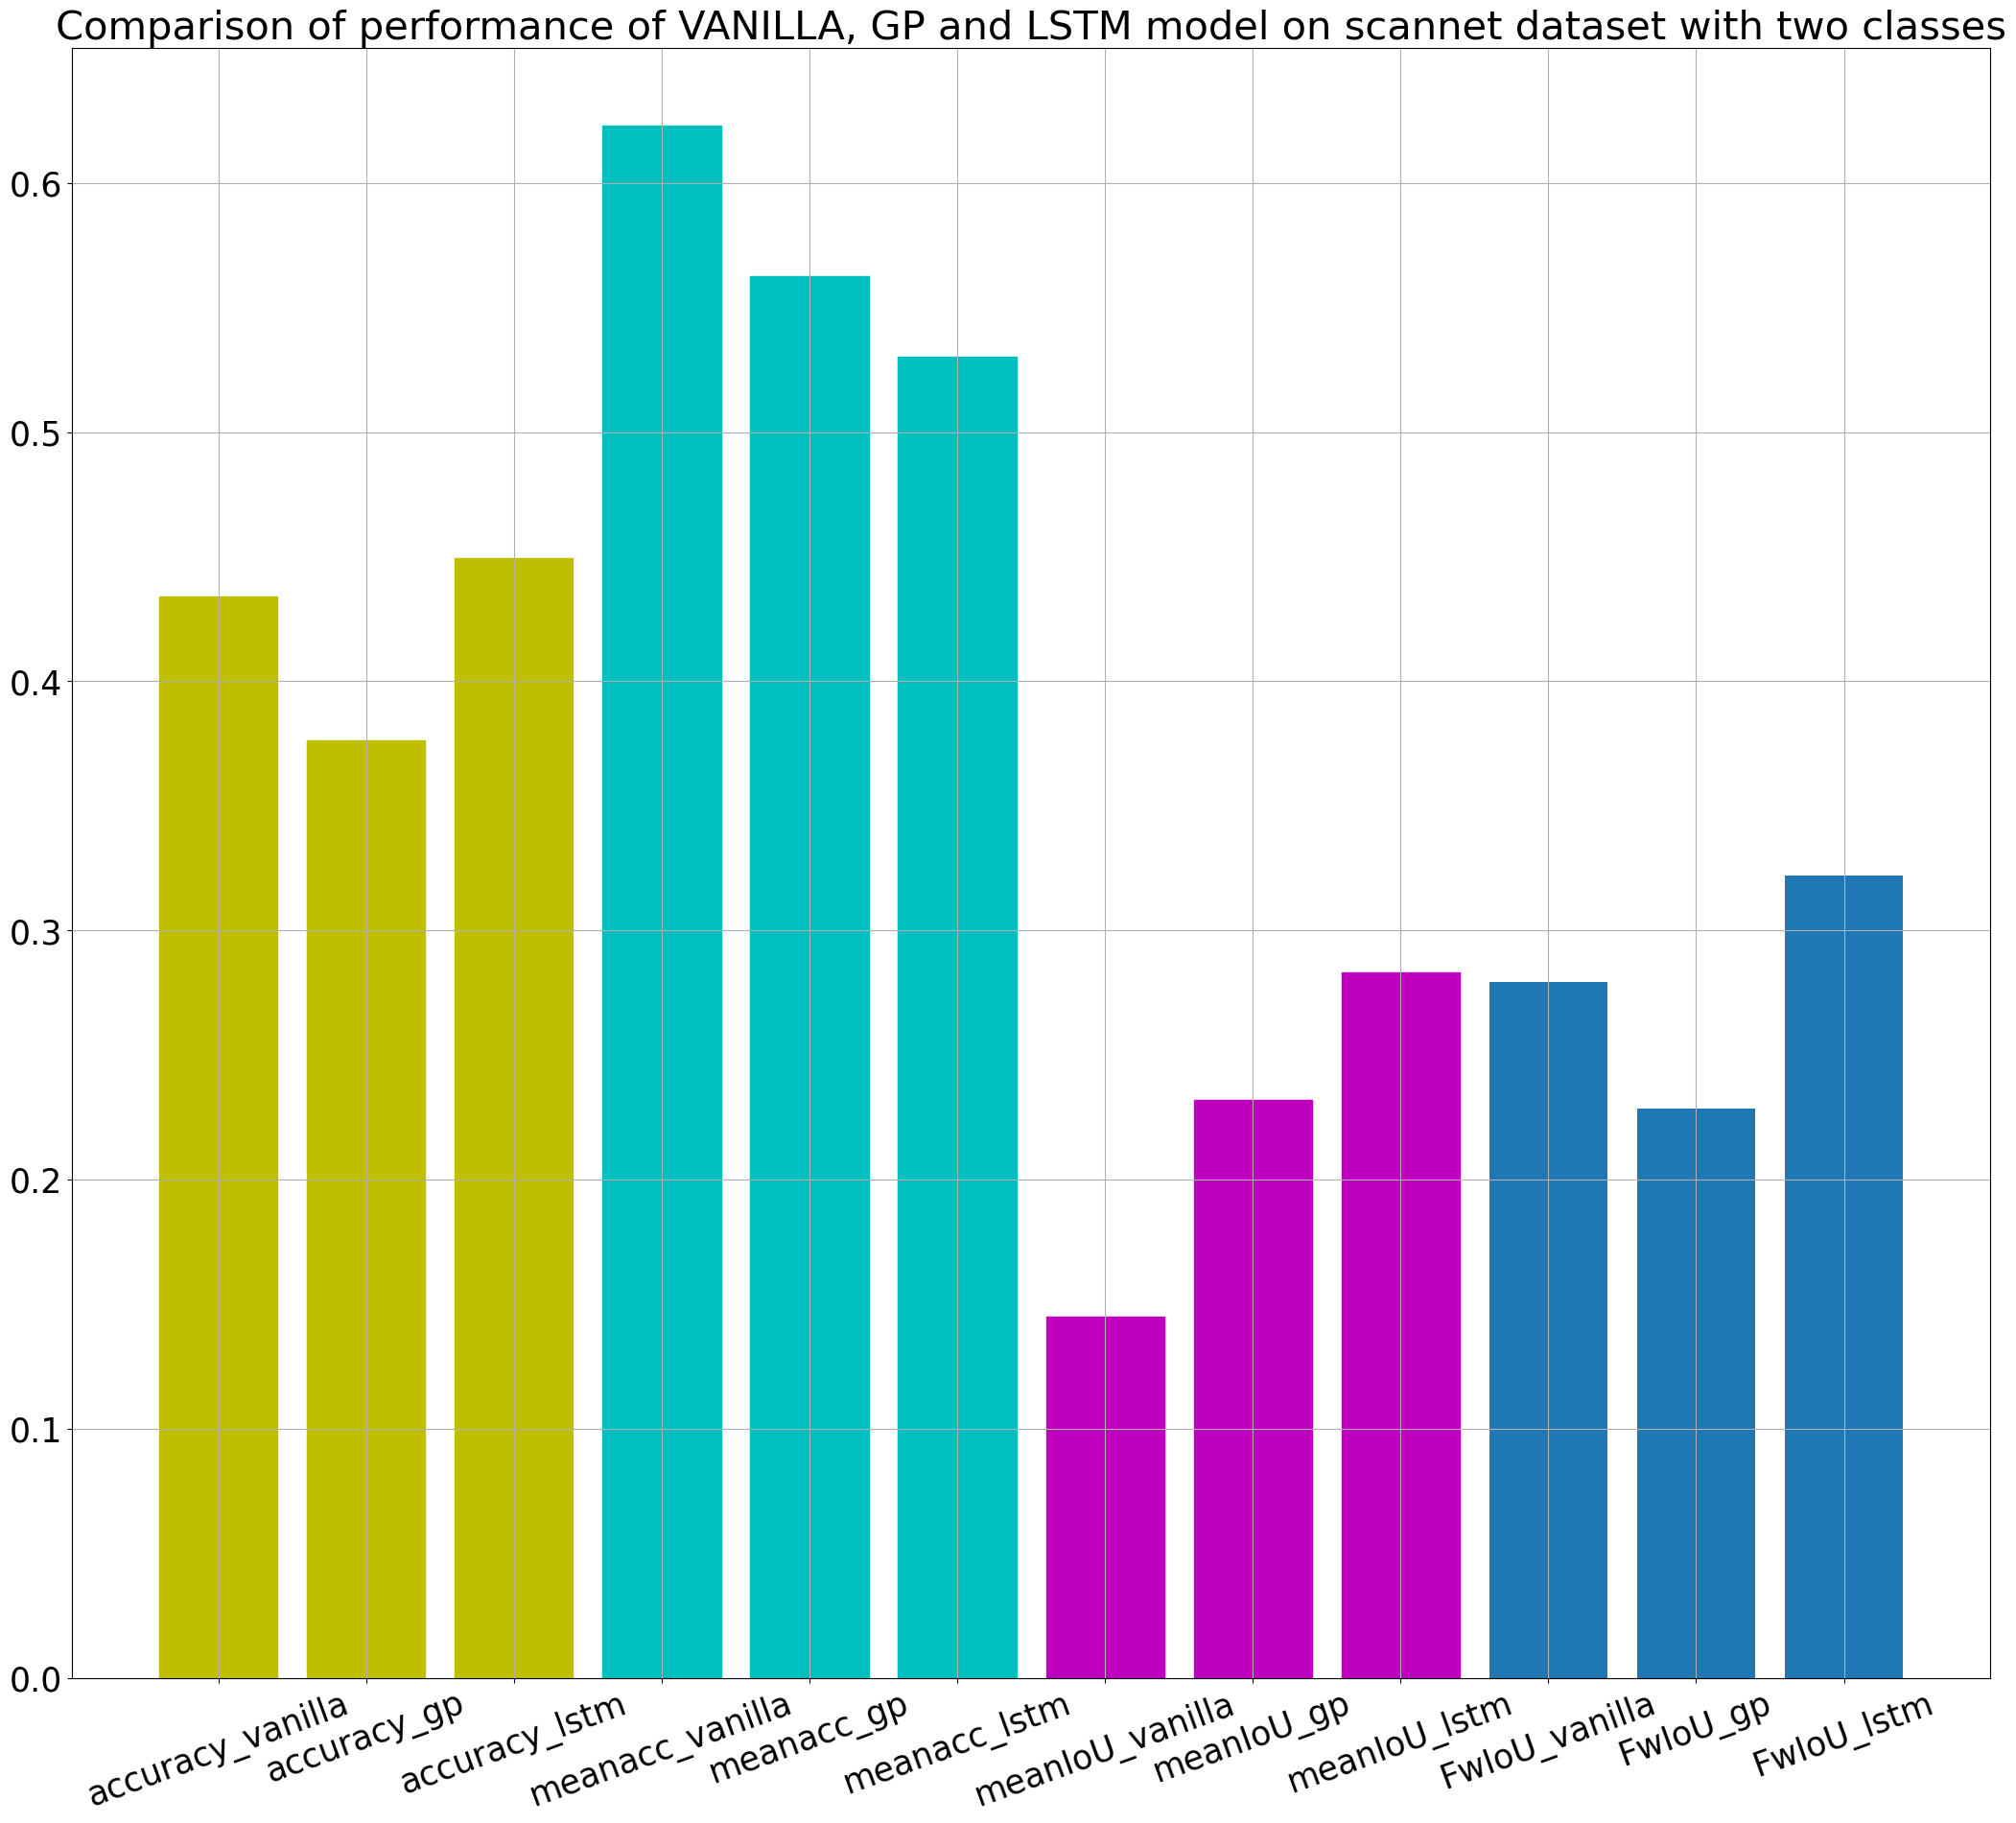
\includegraphics[width=12cm]{images/scannet_performance_two_classes.png}
		\caption{Comparison of VANILLA, GP and LSTM model performance based on metric for scannet two classes}
		\label{fig:unet_model_metric_comparison}
	\end{figure}

    %------------------------------------------------------------------------------------------------------
    \subsection{Experiment1.3: U-Net Vanilla, temporally fused gp and lstm model considering three classes}
	
	This experiment considers wall, furniture, and other combined classes due to high pixel distribution, resulting in three unique classes. There is a massive jump in the pixel accuracy for the lstm and GP models compared to the vanilla model. The mean pixel accuracy is high at 0.55 compared to the vanilla model performance at 0.31. An increase of 24\%. The meanIoU value also stands at 0.40 for the lstm model compared to 0.18 for the vanilla model, a difference of 22\%. The FwIoU value increased by 25\% for the lstm model. The effect of temporal fusion can be clearly seen with these metrics. Temporal fusion improved the performance by a considerable margin. The GP model also performed well in comparison with vanilla and lstm. In this experiment, the pixel classes are well-balanced compared to the two-class approach, where the difference is high. The results are compared in the table Table \ref{table:unet_scannet_three_classes}. In Fig \ref{fig:performance_metric_three_classes_scannet}, there is temporal fusion in action. The comparison of model performance with a bar plot is depicted in Fig \ref{fig:performance_metric_three_classes_unet}
	
	\begin{figure}
		\centering
		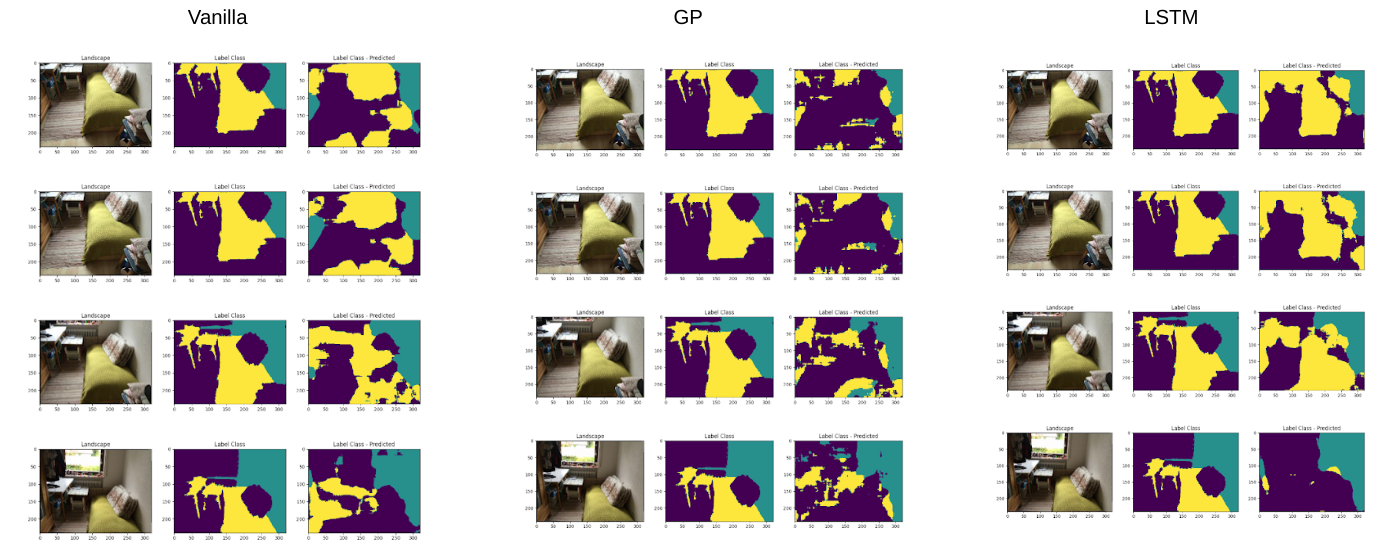
\includegraphics[width=16cm]{images/unet_scannet_three_classes.png}
		\caption{Plotting of raw input image, ground truth and predicted output for vanilla, gp and lstm model}
		\label{fig:performance_metric_three_classes_scannet}
	\end{figure}

	\begin{table}[h]
		\begin{center}
			\begin{tabular}{ | l | l | l | p{4cm} |}
				\hline
				
				\cellcolor{purple!30}Metric & \cellcolor{purple!30}Vanilla & \cellcolor{purple!30}GP & \cellcolor{purple!30}LSTM\\ \hline
				Pixel Accuracy & 0.3289 & 0.5731 & 0.6266 \\ \hline
				Pixel Mean accuracy & 0.3135 & 0.4779 & 0.6920 \\ \hline
				meanIOU & 0.1820 & 0.3356 & 0.4870 \\ \hline
				IoU & [0.2732, 0.1686, 0.1042] & [0.5178, 0.3066, 0.1823] & [0.6810, 0.4661, 0.2998] \\ \hline
				FwIoU & 0.2160 & 0.4033 & 0.6245 \\ \hline
				\hline
			\end{tabular}
			\caption{Performance of Vanilla model with respect to different metric and two classes}
			\label{table:unet_scannet_three_classes}
		\end{center}
	\end{table}	
	
	\begin{figure}
		\centering
		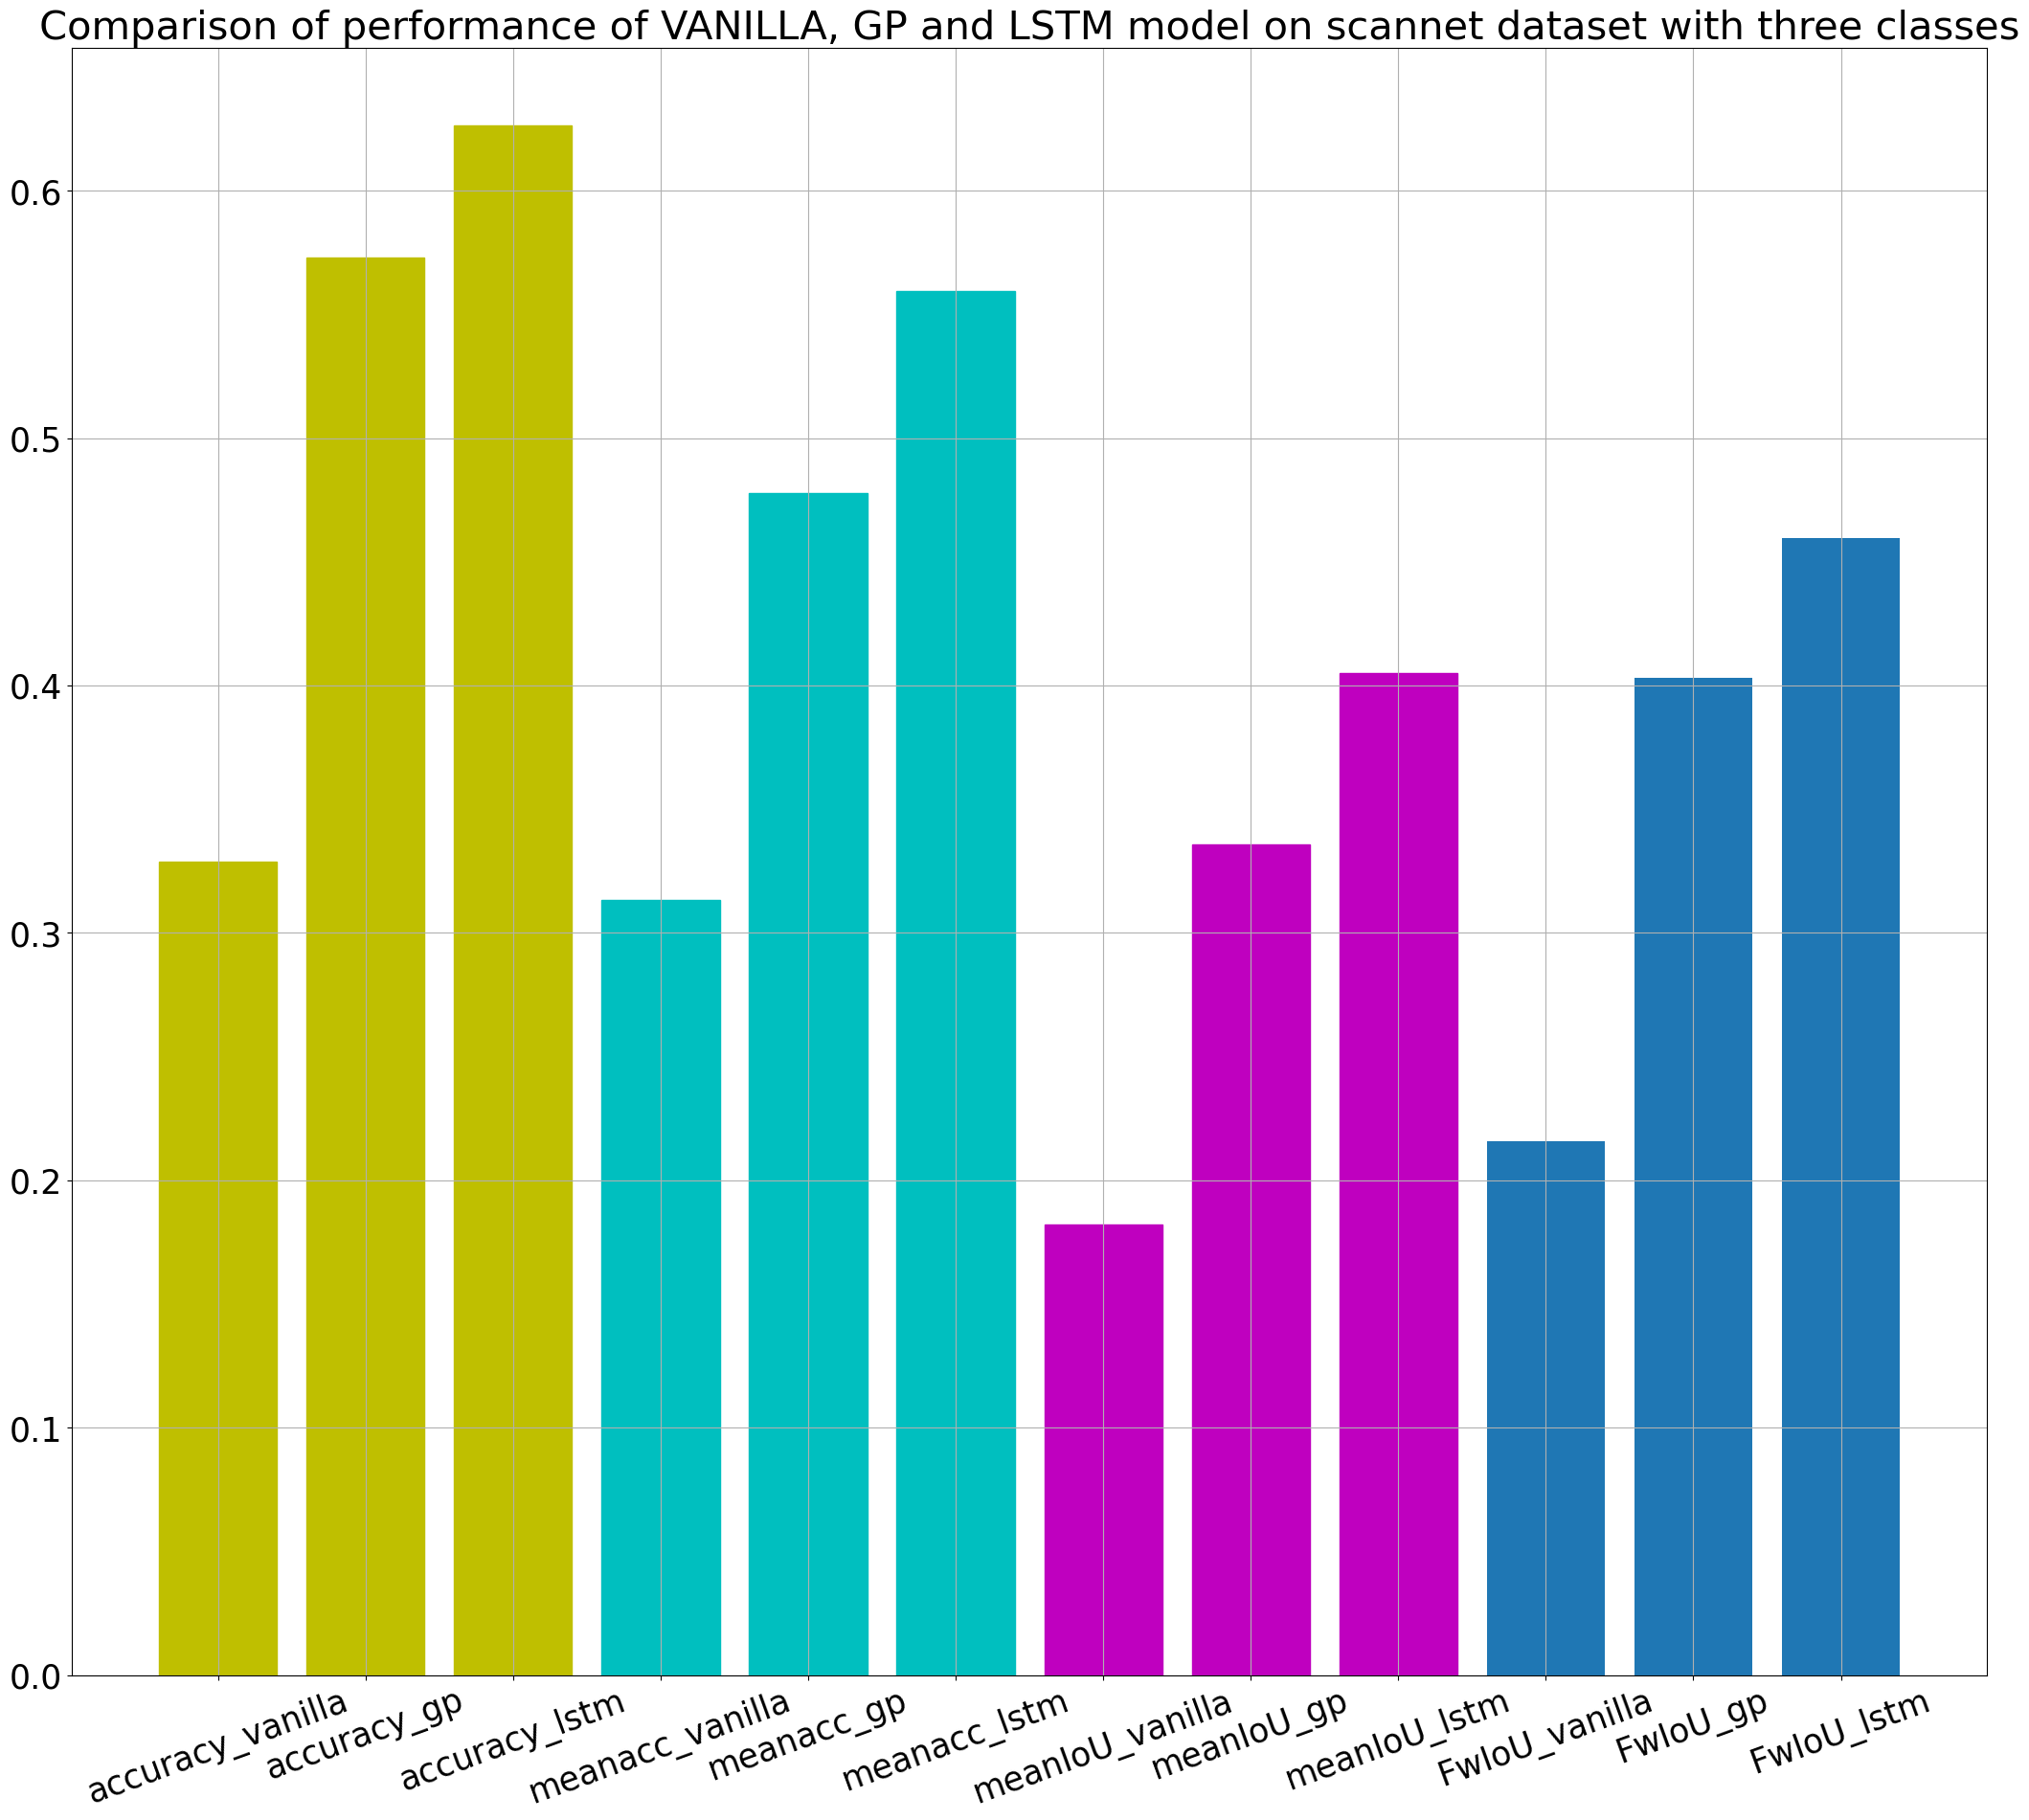
\includegraphics[width=12cm]{images/scannet_performance_three_classes.png}
		\caption{Comparison of VANILLA, GP and LSTM model performance based on metric for scannet three classes}
		\label{fig:performance_metric_three_classes_unet}
	\end{figure}

	\newpage
	\newpage
	%\subsection{Discussion on comparison of results for Vanilla, GP and LSTM models performance}
	
	\section{Experiment 2.1: Experiment with vkitti dataset with fog and morning as the testing data}
	
	Similar to the experiments conducted on the scannet dataset, experiments were conducted on the vkitti dataset. Vkitti is a dataset containing a virtual car moving in a cityscape and recorded with a different configuration. There are a totally of 15 classes in the entire dataset. The results were tabulated in Table \ref{table:unet_vkitti_two_classes}. There are a total of ten categories in the entire dataset. Namely 15-deg-left, fog, overcast, morning, 30-deg-right, 15-deg-right, 30-deg-left, clone, rain, sunset. Under each category, there is a total of 14 classes, namely Terrain, Sky, Tree, Vegetation, Building, Road, GuardRail, TrafficSign, TrafficLight, Pole, Misc, Truck, Car, and Van. In this experiment, fog and morning are taken as the testing data and trained on the remaining eight categories of data.
	The result of the experiments was tabulated in Table \ref{table:unet_vkitti_two_classes}. The Vanilla, GP, and LSTM model performance are compared in the table. Pixel accuracy improved significantly with the LSTM model compared to the Vanilla and Gaussian process. A jump of 11\%. Similar characteristics can be observed concerning the other metrics. All the categories are similar; only the environment changes. A variation in an environment affected the model performance. In this experiment, LSTM performed well compared to the Vanilla and GP models. The accuracy of the model is high, 0.86. Temporal fusion can be observed with mean pixel accuracy, FwIoU, and meanIoU metric with improvement in result. The model is evaluated with the testing data, and the results are calculated for every batch and plotted as the box plot in Fig \ref{fig:performance_metric_vkitti_two_class_box_plot}. For all of the metric, the LSTM produced a better result in comparison to other models. IoU for the building, Misc, and Truck was low with respect to the other classes. The performance of vanilla and the GP model are comparable to each other. Four test images were taken and run through vanilla, GP, and LSTM model, and the ground truth and the predictions were compared side by side. Vanilla and GP models ideally segment the Truck; however, the LSTM model does not correctly segment the Truck. However, the car, pole, road, and sky categories are perfectly categorized by these models. The side-by-side comparison is presented in Figure \ref{fig:vkitti_unet_two}. The experiments were conducted in a batch of 8.
	
	\begin{figure}[h]
		\centering
		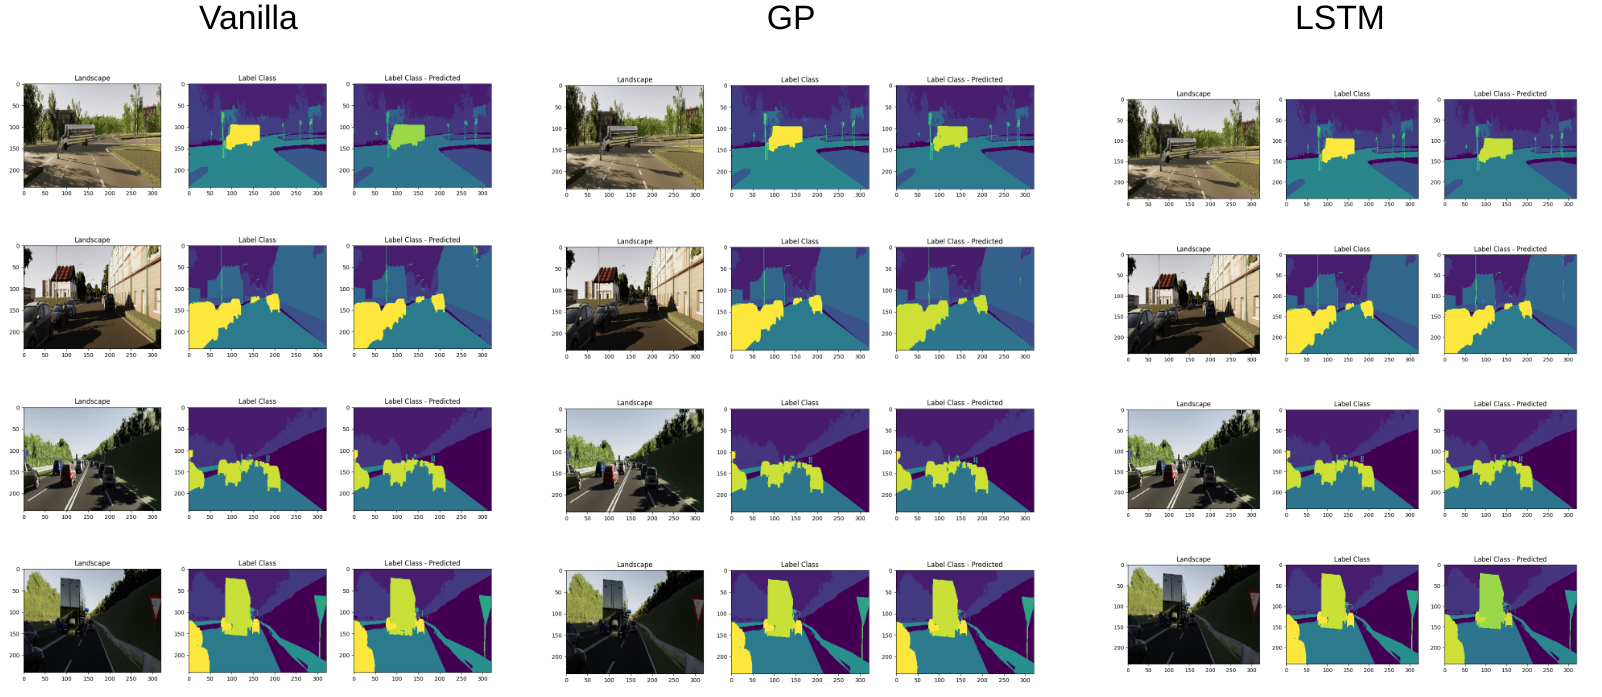
\includegraphics[width=17cm]{images/unet_vkitti_two.png}
		\caption{Plotting of raw input image, ground truth and predicted output for vanilla, gp and lstm for vkitti dataset}
		\label{fig:vkitti_unet_two}
	\end{figure}

	\begin{table}
		\begin{center}
			\begin{tabular}{ | l | p{4cm} | p{4cm} | p{4cm} |}
				\hline
				
				\cellcolor{purple!30}Metric & \cellcolor{purple!30}Vanilla & \cellcolor{purple!30}GP & \cellcolor{purple!30}LSTM\\ \hline
				
				Pixel Accuracy & 0.7423 & 0.7606 & 0.8684 \\ \hline
				Pixel Mean accuracy & 0.6216 & 0.6314 & 0.7449 \\ \hline
				meanIOU & 0.4854 & 0.5122 & 0.6022 \\ \hline
				IoU & [0.5875, 0.7965,	0.5829,	0.4324,	0.1781,	0.7548,	0.6065,	0.5338,	0.2594,	0.3727,	0.2758,	0.2034,	0.8220,	0.3904] & 
				[0.6025,	0.7333,	0.5950, 0.4614,	0.1925,	0.8191,	0.7302,	0.4889,	0.3784,	0.4061,	0.2493,	0.3585,	0.7927,	0.3630] 
				& [ 0.7773,	0.7840,	0.7326,	0.5551,	0.3964,	0.9073,	0.7310,	0.6568,	0.4651,	0.5150,	0.3285,	0.2872,	0.8563,	0.4378]
				\\ \hline
				FwIoU & 0.6451 & 0.6585 & 0.7857 \\ \hline
				\hline
			\end{tabular}
			\caption{Performance of Vanilla model with respect to different metric and two classes}
			\label{table:unet_vkitti_two_classes}
		\end{center}
	\end{table}
	
	\begin{figure}
		\centering
		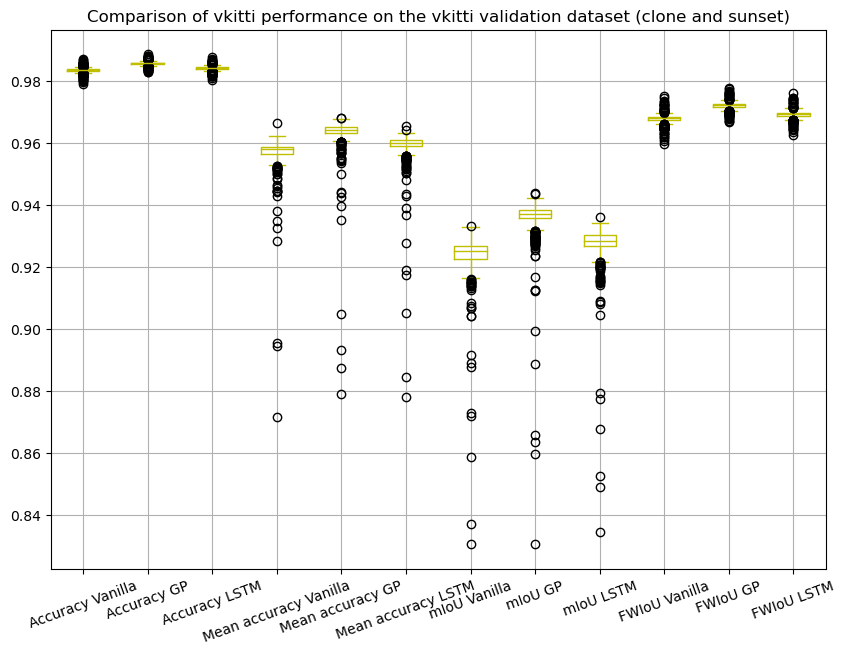
\includegraphics[width=12cm]{images/vkitti_validation_data_two_class_box_plot.png}
		\caption{Performance comparison of the VANILLA, GP and LSTM model based on different metrics}
		\label{fig:performance_metric_vkitti_two_class_box_plot}
	\end{figure}
	
	\begin{figure}
		\centering
		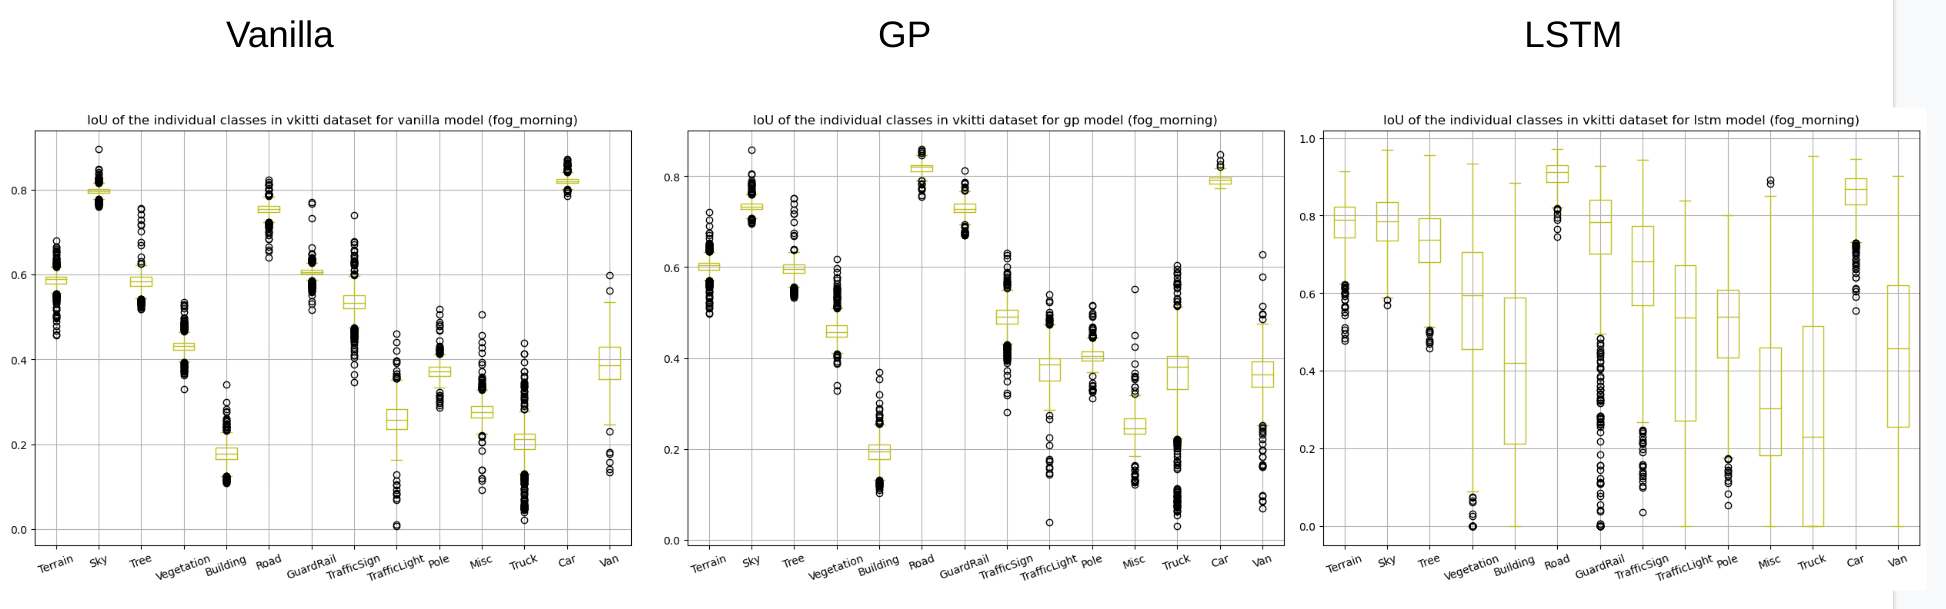
\includegraphics[width=19cm]{images/IoU_two.png}
		\caption{IoU predictions for all the classes for VANILLA, GP and LSTM model}
		\label{fig:performance_metric_three_classes}
	\end{figure}

	\begin{figure}
		\centering
		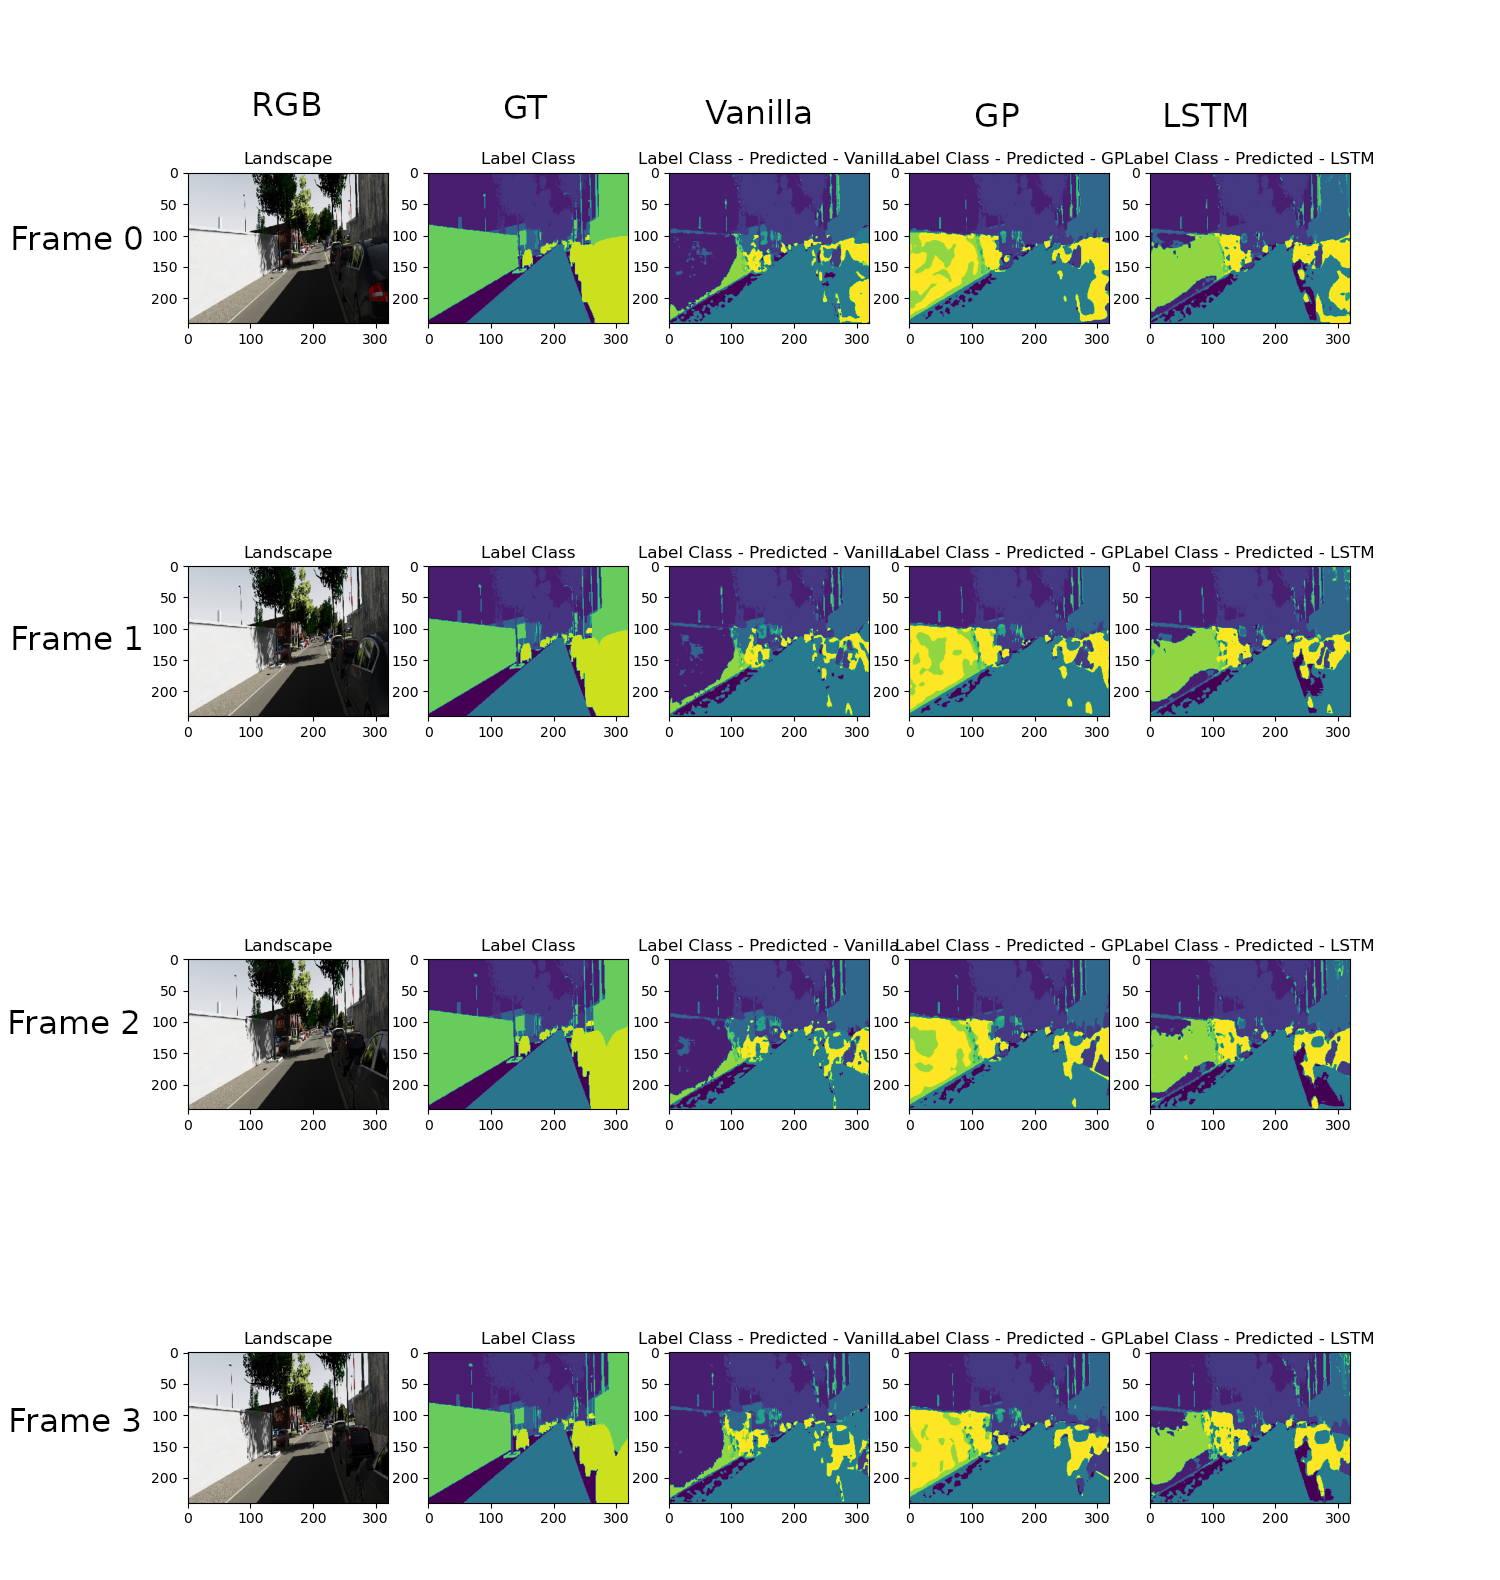
\includegraphics[width=19cm]{images/continuous_sequence_data1.png}
		\caption{Side by side comparison of models predictions for continuous sequence data from frame 1 to 4}
		\label{fig:performance_metric_three_classes}
	\end{figure}

	\begin{figure}
		\centering
		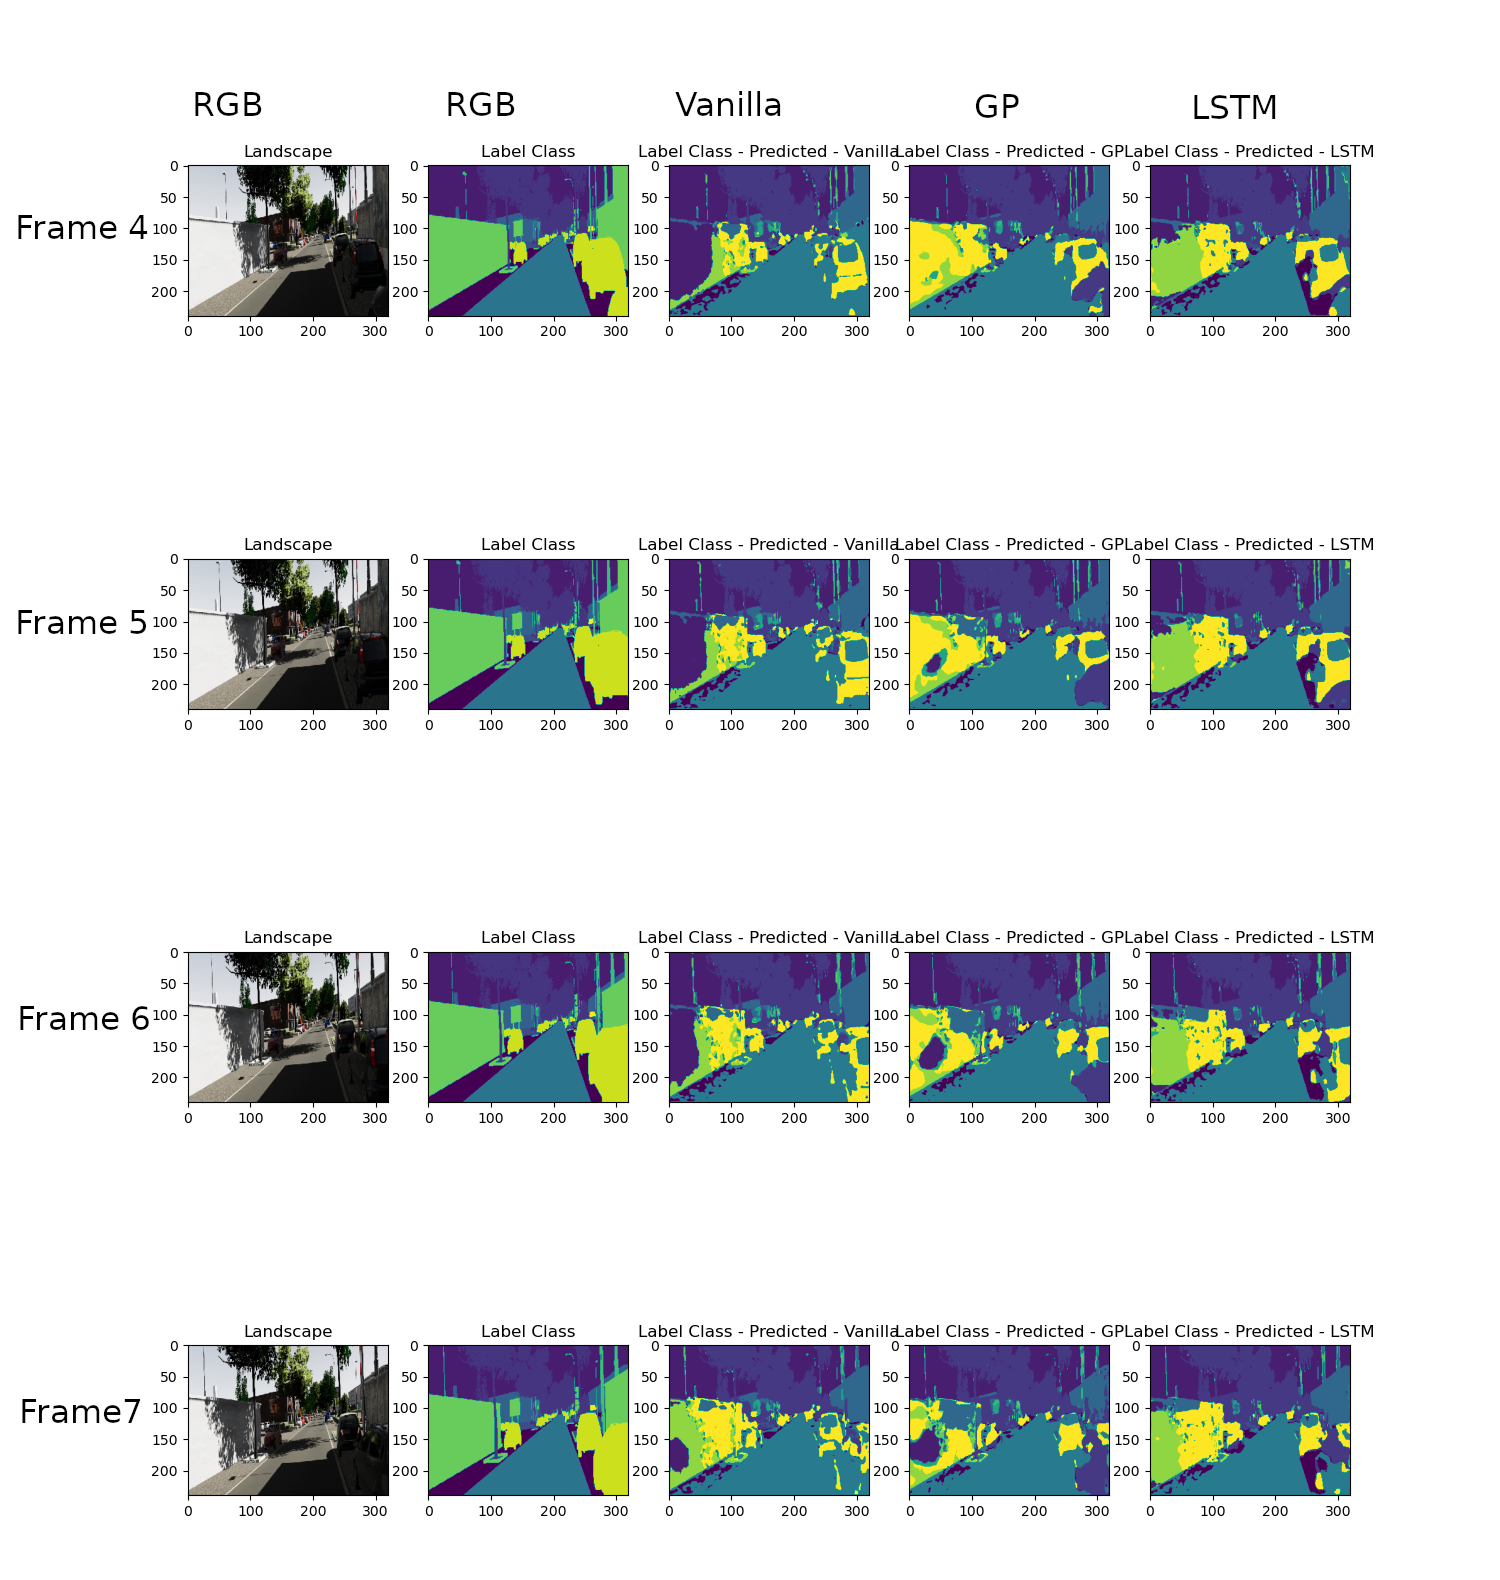
\includegraphics[width=19cm]{images/continuous_sequence_data2.png}
		\caption{Side by side comparison of models predictions for continuous sequence data from frame 5 to 8}
		\label{fig:performance_metric_three_classes}
	\end{figure}

	\subsection{Experiment 2.1.2: Impact of training data batch size on the evaluation dataset performance}
	
	The neural network model can be trained in batch data. The impact of the batch is studied in this experiment. The temporal fusion aims to pass continuous sequence image data and model the temporal dependency resulting in improved performance. In this experiment, a batch of 1, 2, and 8 data are passed onto the temporal fusing neural network model to train and evaluate the performance. In a batch mode of 1, the information from each frame is passed onto the next frame temporally. At a time single image is passed to the network for learning. Two images are passed in the batch mode of 2 at a time, and temporal information from these two images is learned and passed onto the subsequent two frames' prediction. In a batch mode of 8 at a time, a total of 8 image segmentation are learned from the ground truth. The overlapping information present in the set of 8 images is passed onto the following eight sets of continuous sequence data at a time processing eight images. With this experiment, it is found that the performance improves as the number of images in a batch; in other words, as the batch size increases, the performance improves. The same can be observed with the comparison of model performance on a batch size of 1, 2, and 8 in Figure \ref{fig:batch_wise_performance}. However, there is a limitation to the number of images in a batch. In the experiment, a maximum of 8 images per batch was tried; if the batch size increases above eight, the Cuda memory overflow is observed. This is a limitation set by the hardware. 

	\begin{figure}
		\centering
		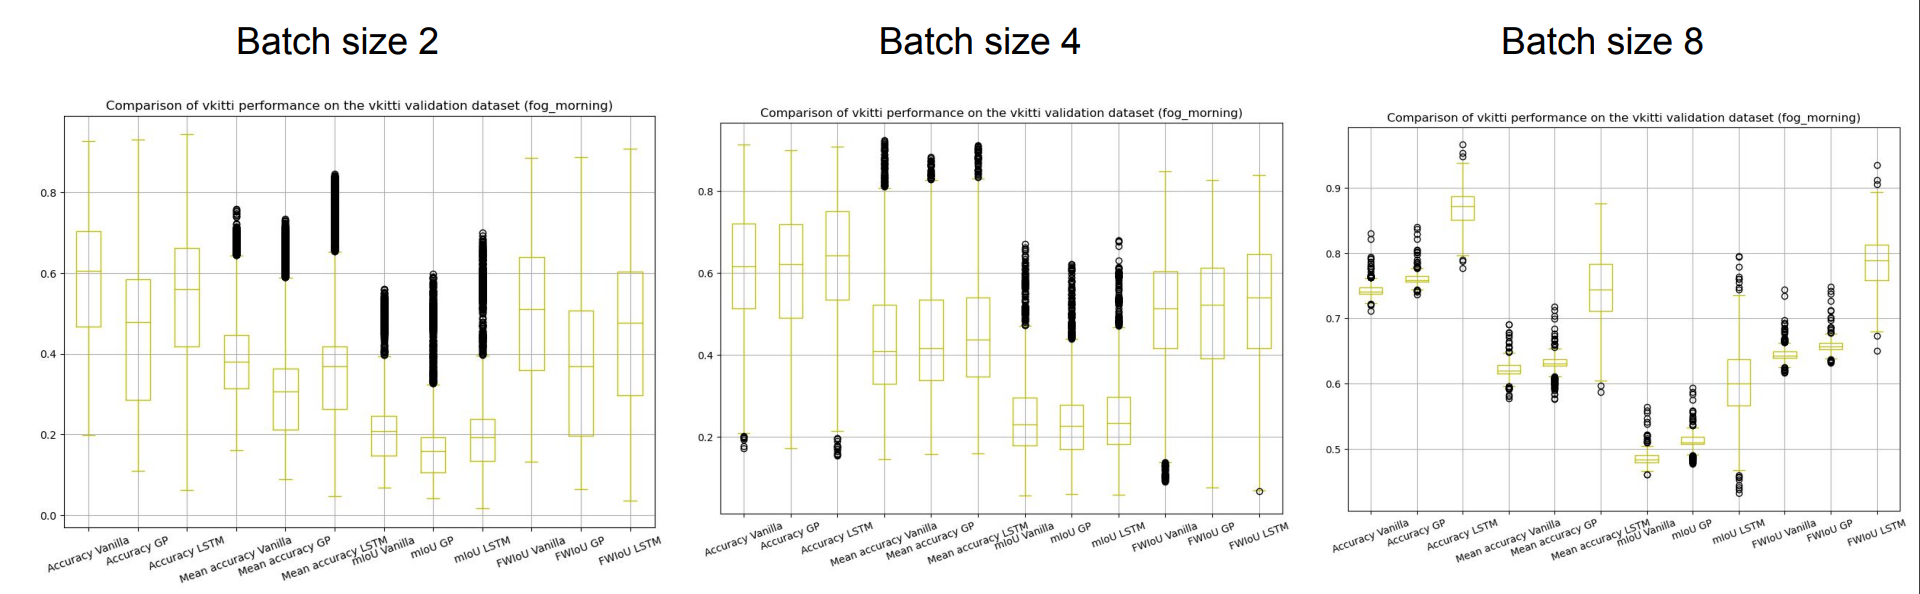
\includegraphics[width=16cm]{images/batch_wise_performance_comparison.png}
		\caption{Impact of training batch size on the evaluation dataset prediction}
		\label{fig:batch_wise_performance}
	\end{figure}		    
	
	\section{Experiment 2.2: Experiment with vkitti dataset with clone, sunset, rain, 15-deg-right, and 30-deg-left as the testing data}
		
	In the second type of experiment on vkitti data, five('clone/', 'sunset/', 'rain/', '15-deg-right/',
	'30-deg-left/') categories out of 10 categories are taken for testing. The model is trained on five (15-deg-left/','fog/', 'overcast/', 'morning/', and '30-deg-right/') categories. The result of the experiments is tabulated in Table \ref{table:Vanilla_conti_seq}. It is a side-by-side comparison of the model performance based on a different metric. The performance improvement can be observed with the menIoU metric. The meanIoU improved by 1\% and 3\% for GP and lstm with respect to the vanilla model. Similar characteristics can be observed with the mean pixel accuracy. However, the pixel accuracy remained constant for all three models. The side-by comparison of the raw RGB image, ground truth, and predicted segmentation map is shown in Fig \ref{fig:unet_side_by_side_five_classes}. 
	
	\begin{figure}
		\centering
		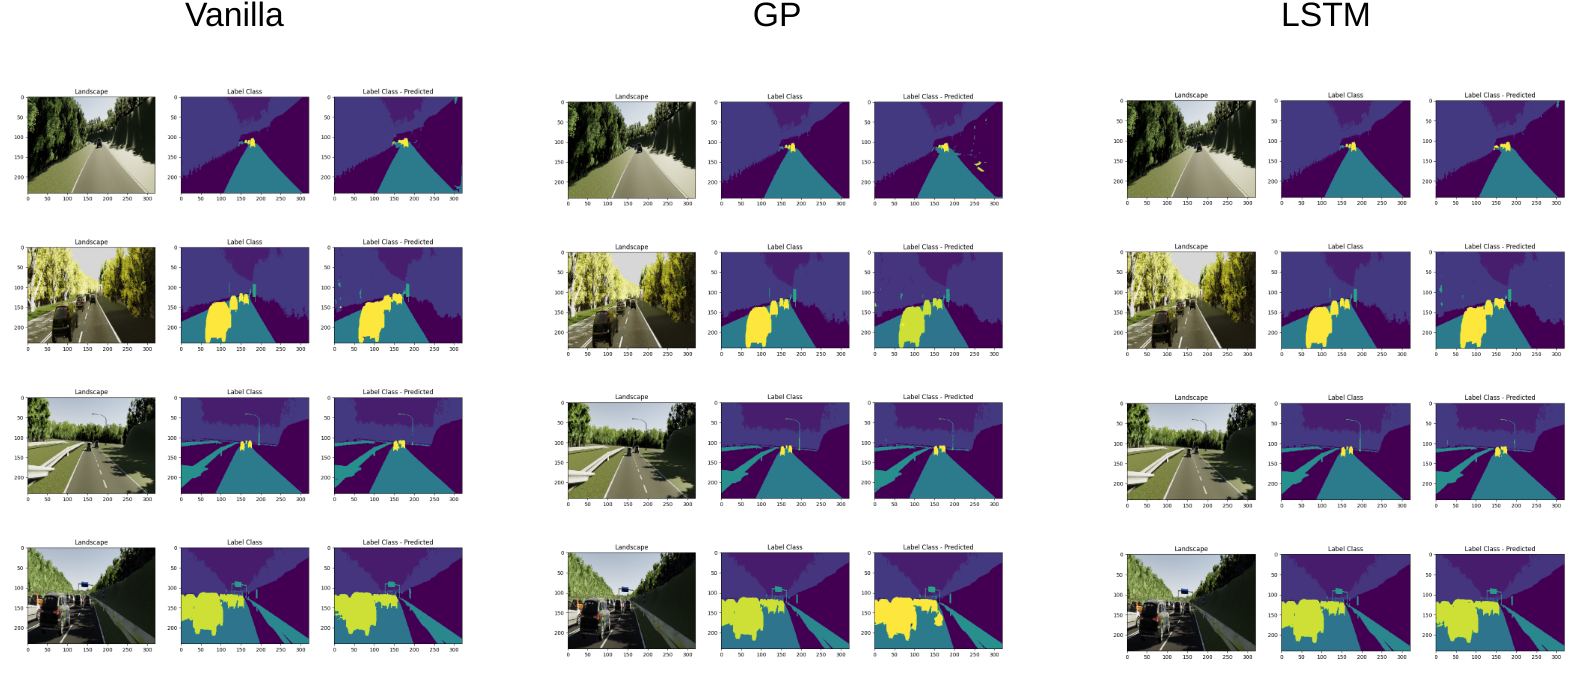
\includegraphics[width=17cm]{images/unet_vkitti_five.png}
		\caption{Plotting of raw input image, ground truth and predicted output for vanilla, gp and lstm}
		\label{fig:unet_side_by_side_five_classes}
	\end{figure}

	\begin{table}
		\begin{center}
			\begin{tabular}{ | l | p{4cm} | p{4cm} | p{4cm} |}
				\hline
				
				\cellcolor{purple!30}Metric & \cellcolor{purple!30}Vanilla & \cellcolor{purple!30}GP & \cellcolor{purple!30}LSTM\\ \hline
				Pixel Accuracy & 0.9419 & 0.9329 & 0.9491 \\ \hline
				Pixel Mean accuracy & 0.7797 & 0.7878 & 0.8083 \\ \hline
				meanIOU & 0.6884 & 0.6977 & 0.7206 \\ \hline
				IoU & [0.9128, 0.9417, 0.92, 0.6876, 0.7247, 0.958, 0.8576, 0.6196, 0.4536, 0.4217, 0.3476, 0.5452, 0.8674, 0.3803] & 
				[0.8961, 0.8985, 0.8949, 0.7113, 0.7408, 0.9505, 0.8602, 0.6862, 0.5612, 0.4683, 0.3427, 0.4788, 0.8506, 0.4285]
				& [0.9078, 0.9565, 0.9296, 0.7427, 0.7816, 0.96, 0.8669, 0.6828, 0.4898, 0.4464, 0.4182, 0.6187, 0.8843, 0.4025]
				\\ \hline
				FwIoU & 0.8959 & 0.8788 & 0.9074 \\ \hline
				\hline
			\end{tabular}
			\caption{Performance of Vanilla model with respect to different metric and two classes}
			\label{table:Vanilla_conti_seq}
		\end{center}
	\end{table}
	
	The box plot of the performance of the vanilla, GP, and lstm model is shown in Fig \ref{fig:performance_metric_unet}. The pixel accuracy and  FwIoU are high for the lstm model, and the performance is comparable for the GP and vanilla models. Mean pixel accuracy and meanIoU are high for the lstm model. Traffic light, Pole, and Misc class IoU are low in vanilla, GP, and lstm models. The same is shown in Fig \ref{fig:performance_metric_three_classes_unet_five}. Hence from the result table, we can prove that incorporating the temporal fusion data for the semantic segmentation improves the performance. 
	
	\begin{figure}[h]
		\centering
		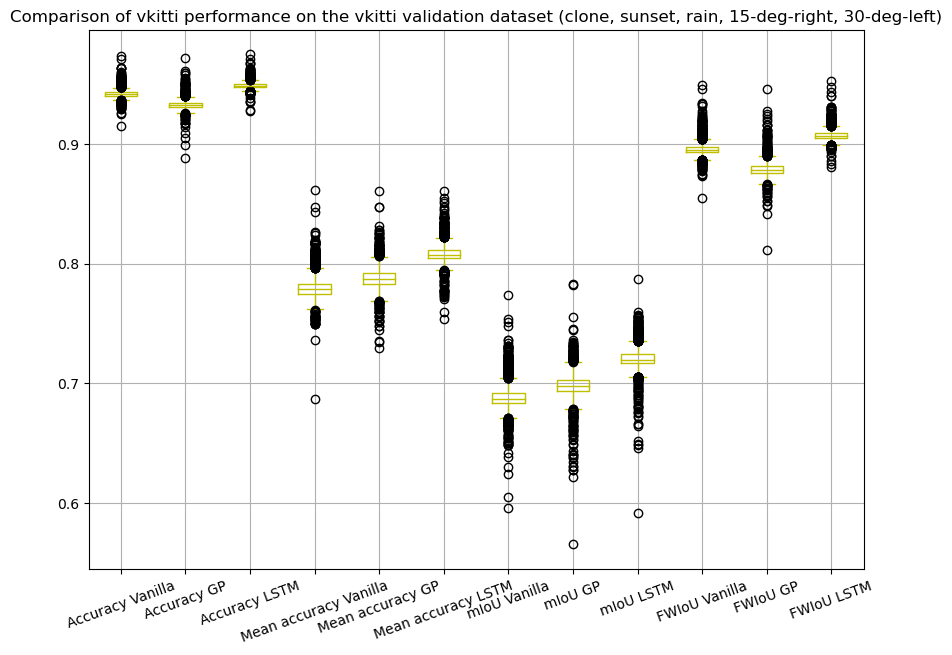
\includegraphics[width=12cm]{images/vkitti_validation_data_five_class_box_plot.png}
		\caption{Comparison of model performance based on different metrics}
		\label{fig:performance_metric_unet}
	\end{figure}
	
	\begin{figure}
		\centering
		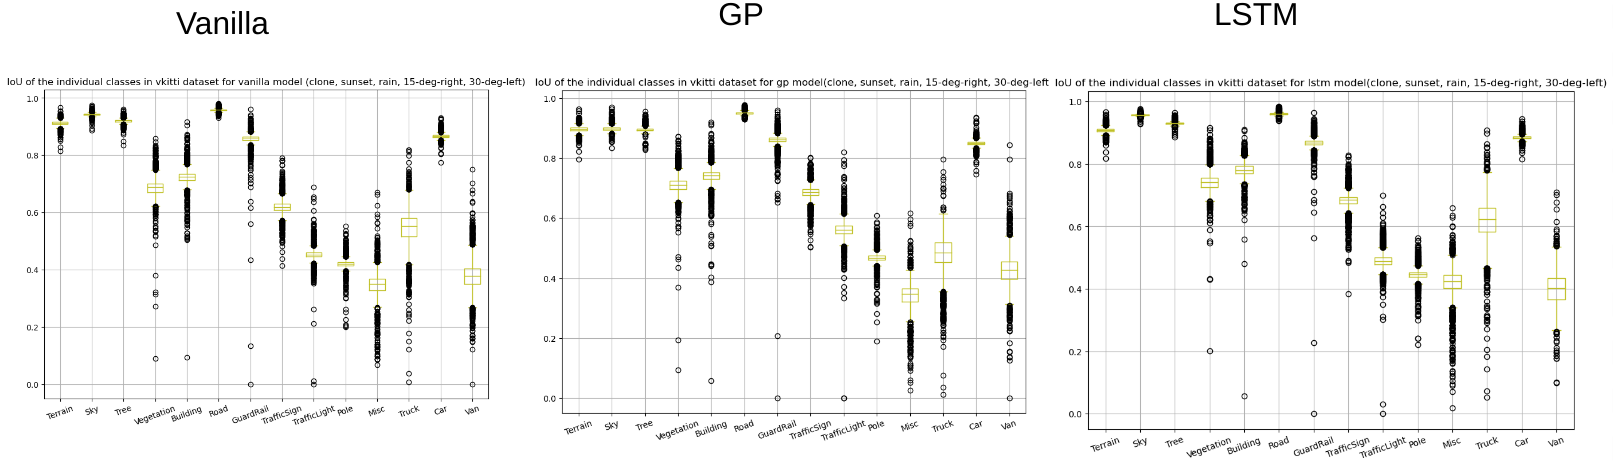
\includegraphics[width=19cm]{images/IoU_five.png}
		\caption{IoU for all the classes in the dataset with respect to different model predictions}
		\label{fig:performance_metric_three_classes_unet_five}
	\end{figure}
	
	
	\section{Comments and Discussion}   
	
	The Long Short-Term Memory (LSTM) model outperformed the performance of the vanilla/baseline and Gaussian Process (GP) models. The LSTM model can effectively model long temporal data, and the Gaussian Process (GP) uses pose information to model temporal data. The GP method is adopted from the depth estimation approach, where a cost volume is generated by taking consecutive frames. This cost volume captures the overlapping information present in the consecutive frames. However, building a cost volume is optional for semantic segmentation, as it is specifically designed for the depth estimation task.
	However, a modified GP approach is performed by subjecting the latent space encoding to GP and averaging the previous latent space encoding that was subjected to GP with the current latent space encoding.
	
%	\newpage
%	
%	\section{Benchmarking of results for scannet dataset and vkitti dataset}
%	
%	{ \bf Scannet dataset}
%	
%	The table \ref{table:scannet_benchmark} lists all the state of the art semantic segmentation model performance. The best average iou for the entire scannet dataset is 0.745. In this model 
%	
%	The pixel accuracy is 50.96\% for the validation dataset. The is due to the presence of large number of classes with unequal pixel distribution. However, the IoU for the Wall, Floor and Mattress is high at 0.56, 0.608, 0.382 due to the high pixel distribution for these classes. Frequency weighted IoU take into account the unequal pixel distribution and the values stand at 0.3531. The predicted and the ground truth pixel distribution is presented in the Fig \ref{fig:y_gt_pred_vanilla}.
%	
%	The pixel accuracy is 50.96\% for the validation dataset. The is due to the presence of large number of classes with unequal pixel distribution. However, the IoU for the Wall, Floor and Mattress is high at 0.56, 0.608, 0.382 due to the high pixel distribution for these classes. Frequency weighted IoU take into account the unequal pixel distribution and the values stand at 0.3531. The predicted and the ground truth pixel distribution is presented in the Fig \ref{fig:y_gt_pred_vanilla}. Frequency weighted IoU take into account the unequal pixel distribution and the values stand at 0.3531. The predicted and the ground truth pixel distribution is presented in the Fig \ref{fig:y_gt_pred_vanilla}.
%	Frequency weighted IoU take into account the unequal pixel distribution and the values stand at 0.3531. The predicted and the ground truth pixel distribution is presented in the Fig \ref{fig:y_gt_pred_vanilla}.Frequency weighted IoU take into account the unequal pixel distribution and the values stand at 0.3531. The predicted and the ground truth pixel distribution is presented in the Fig \ref{fig:y_gt_pred_vanilla}.
	
%	\begin{table}[h]
%		\begin{center}
%			\begin{tabular}{ | l | l | l | l| p{4cm} |}
%				\hline
%				
%				\cellcolor{purple!30}Method & \cellcolor{purple!30}Avg iou & \cellcolor{purple!30} Pixel Accuracy & \cellcolor{purple!30} Mean Pixel Accuracy & \cellcolor{purple!30} FwIoU \\ \hline
%				
%				Virtual MVFusion (R) & 0.745 & - & - & -  \\ \hline
%				BPNet\_2D & 0.67 & - & - & -  \\ \hline
%				CU-Hybrid-2D Net & 0.636  & - & - & -  \\ \hline
%				CMX & 0.613 & - & - & -  \\ \hline
%				DMMF\_3d & 0.605 & - & -  & - \\ \hline
%				MCA-Net & 0.595 & - & -  & - \\ \hline
%				RFBNet & 0.592 & - & -  & - \\ \hline
%				DCRedNet & 0.583 & -  & - & - \\ \hline
%				SSMA & 0.577 & - & -  & - \\ \hline
%				SN\_RN152pyrx8\_RVC & 0.546 & - & - & - \\ \hline
%				FuseNet & 0.535 & - & -  & - \\ \hline
%				AdapNet++ & 0.503 & - & -  & - \\ \hline
%				3DMV (2d proj) & 0.498 & - & - & - \\ \hline
%				MSeg1080\_RVC & 0.485 & -  & - & - \\ \hline
%				ILC-PSPNet & 0.475 & - & - & - \\ \hline
%				Enet & 0.376 & - & - & - \\ \hline
%				ScanNet & 0.33 & - & - & - \\ \hline
%				LSTM Unet & 0.145 & - & -  & - \\ \hline
%				GP Unet & 0.1161  & - & - & - \\ \hline
%				Vanilla Unet & 0.112 & - & - & - \\ \hline
%			
%				\hline
%			\end{tabular}
%			\caption{Comparison of model performance on the Scannet data}
%			\label{table:scannet_benchmark}
%		\end{center}
%	\end{table}	
%	
%	\newpage
%	
%	{ \bf Vkitti dataset, refer: https://arxiv.org/pdf/2006.04080v2.pdf}
%	
%	The pixel accuracy is 50.96\% for the validation dataset. The is due to the presence of large number of classes with unequal pixel distribution. However, the IoU for the Wall, Floor and Mattress is high at 0.56, 0.608, 0.382 due to the high pixel distribution for these classes. Frequency weighted IoU take into account the unequal pixel distribution and the values stand at 0.3531. The predicted and the ground truth pixel distribution is presented in the Fig \ref{fig:y_gt_pred_vanilla}. Frequency weighted IoU take into account the unequal pixel distribution and the values stand at 0.3531. The predicted and the ground truth pixel distribution is presented in the Fig \ref{fig:y_gt_pred_vanilla}.
%	Frequency weighted IoU take into account the unequal pixel distribution and the values stand at 0.3531. The predicted and the ground truth pixel distribution is presented in the Fig \ref{fig:y_gt_pred_vanilla}.Frequency weighted IoU take into account the unequal pixel distribution and the values stand at 0.3531. The predicted and the ground truth pixel distribution is presented in the Fig \ref{fig:y_gt_pred_vanilla}.
	
%	\begin{table}[h]
%		\begin{center}
%			\begin{tabular}{ | l | l | l | l| p{4cm} |}
%				\hline
%				
%				\cellcolor{purple!30}Method & \cellcolor{purple!30}Avg iou & \cellcolor{purple!30} Pixel Accuracy & \cellcolor{purple!30} Mean Pixel Accuracy & \cellcolor{purple!30} FwIoU \\ \hline
%				
%				Virtual MVFusion (R) & 0.745 & - & - & -  \\ \hline
%				BPNet\_2D & 0.67 & - & - & -  \\ \hline
%				CU-Hybrid-2D Net & 0.636  & - & - & -  \\ \hline
%				CMX & 0.613 & - & - & -  \\ \hline
%				DMMF\_3d & 0.605 & - & -  & - \\ \hline
%				MCA-Net & 0.595 & - & -  & - \\ \hline
%				RFBNet & 0.592 & - & -  & - \\ \hline
%				DCRedNet & 0.583 & -  & - & - \\ \hline
%				SSMA & 0.577 & - & -  & - \\ \hline
%				SN\_RN152pyrx8\_RVC & 0.546 & - & - & - \\ \hline
%				FuseNet & 0.535 & - & -  & - \\ \hline
%				AdapNet++ & 0.503 & - & -  & - \\ \hline
%				3DMV (2d proj) & 0.498 & - & - & - \\ \hline
%				MSeg1080\_RVC & 0.485 & -  & - & - \\ \hline
%				ILC-PSPNet & 0.475 & - & - & - \\ \hline
%				Enet & 0.376 & - & - & - \\ \hline
%				ScanNet & 0.33 & - & - & - \\ \hline
%				Vanilla Unet & 0.112 & - & - & - \\ \hline
%				GP Unet & 0.1161  & - & - & - \\ \hline
%				LSTM Unet & 0.145 & - & -  & - \\ \hline
%				\hline
%			\end{tabular}
%			\caption{Comparison of model performance on the Scannet data}
%			\label{table:LSTM_conti_seq}
%		\end{center}
%	\end{table}
    
\end{document}
